\documentclass[10pt, french]{book}

\usepackage[T1]{fontenc}
\usepackage[utf8]{inputenc}
\usepackage[french]{babel}
\usepackage{microtype}

\usepackage{tikz}
\usetikzlibrary{positioning}

\usepackage{amsmath, amsfonts}
\usepackage{lmodern}
\fontfamily{lmr}\selectfont

\usepackage{geometry}
\geometry{
  headsep=4mm,
  papersize={17.5cm,24cm},
  top=18mm,
  bottom=18mm,
  left=26mm,
  right=18mm
}

\setlength{\parindent}{0pt}

\usepackage{colortbl}


%%% Style d'en-tête %%%

\usepackage{fancyhdr}
\fancypagestyle{plain}{\fancyhf{}\renewcommand{\headrulewidth}{0pt}}

\pagestyle{fancy}
\fancyhf{}
\setlength{\headheight}{\baselineskip}
% \renewcommand{\headrulewidth}{.6cm}

\renewcommand{\sectionmark}[1]{\markright{#1}}
\renewcommand{\chaptermark}[1]{\markboth{\chaptername~\thechapter~:~#1}{}}

\fancyhead[OL]{\it\nouppercase\rightmark}
\fancyhead[OR]{\it\thepage}

\fancyhead[EL]{\it\thepage}
\fancyhead[ER]{\it\nouppercase\leftmark}

% Pas d'en-tête sur les pages avant chaque chapitre
\makeatletter
\def\cleardoublepage{\clearpage\if@twoside \ifodd\c@page\else
    \hbox{}
    \thispagestyle{plain}
    \newpage
    \if@twocolumn\hbox{}\newpage\fi\fi\fi}
\makeatother \clearpage{\pagestyle{plain}\cleardoublepage}


%%% Style des titres %%%

\usepackage{titlesec}

\newlength\chapnumb
\setlength\chapnumb{3cm}

% Chapitres
\titleformat{\chapter}{}{}{0pt} {
  \raggedleft
  \fontsize{3.8cm}{0pt}\selectfont\thechapter\\
  \vspace*{3cm}
  \fontsize{25pt}{0pt}\sl\bfseries\selectfont
}
\titlespacing*{\chapter}{0pt}{0pt}{1cm}

% Parties
\titleformat{\section}{\sl\LARGE\bfseries}{\thesection}{\fontdimen2\font}{}


%%% Style des listes %%%

\frenchsetup{StandardItemLabels=true}

\usepackage{enumitem}
\setlist[itemize]{left=0pt..8mm}


%%% Style des blocs de code %%%

\usepackage{listingsutf8}

\lstalias{text}{}
% \newcommand{\ColorLang}{caml}
\newcommand{\ColorLang}{text}

\lstset{
  inputencoding=utf8/latin1,
  basicstyle=\ttfamily,
  basewidth=0.5em,
  language=\ColorLang,
  % frame=single
}

\newcommand{\SourceFile}{}


%%% Définitions de macros %%%

\newcounter{question}[section] % Remis à 0 à chaque nouvelle section
\newcommand{\Q}{
  \stepcounter{question}
  \vspace{.4cm}
  {\sffamily Question \arabic{question}}
  \vspace{.4cm}\\
}

\newcommand{\Corrige}{
  \setcounter{question}{0}
  \vspace{1cm}
  \centerline{\sffamily \rule[0.6ex]{2cm}{.1mm} CORRIGÉ \rule[0.6ex]{2cm}{.1mm}}
  \vspace{-.4cm}
}

\newcommand{\Epigraph}[1]{
  \og{\it#1}\fg
}

\newcommand{\Fin}{
  \centerline{$\star\star\star\star\star\star\star\star$}
}


\begin{document}
    \raggedbottom
    \frontmatter

    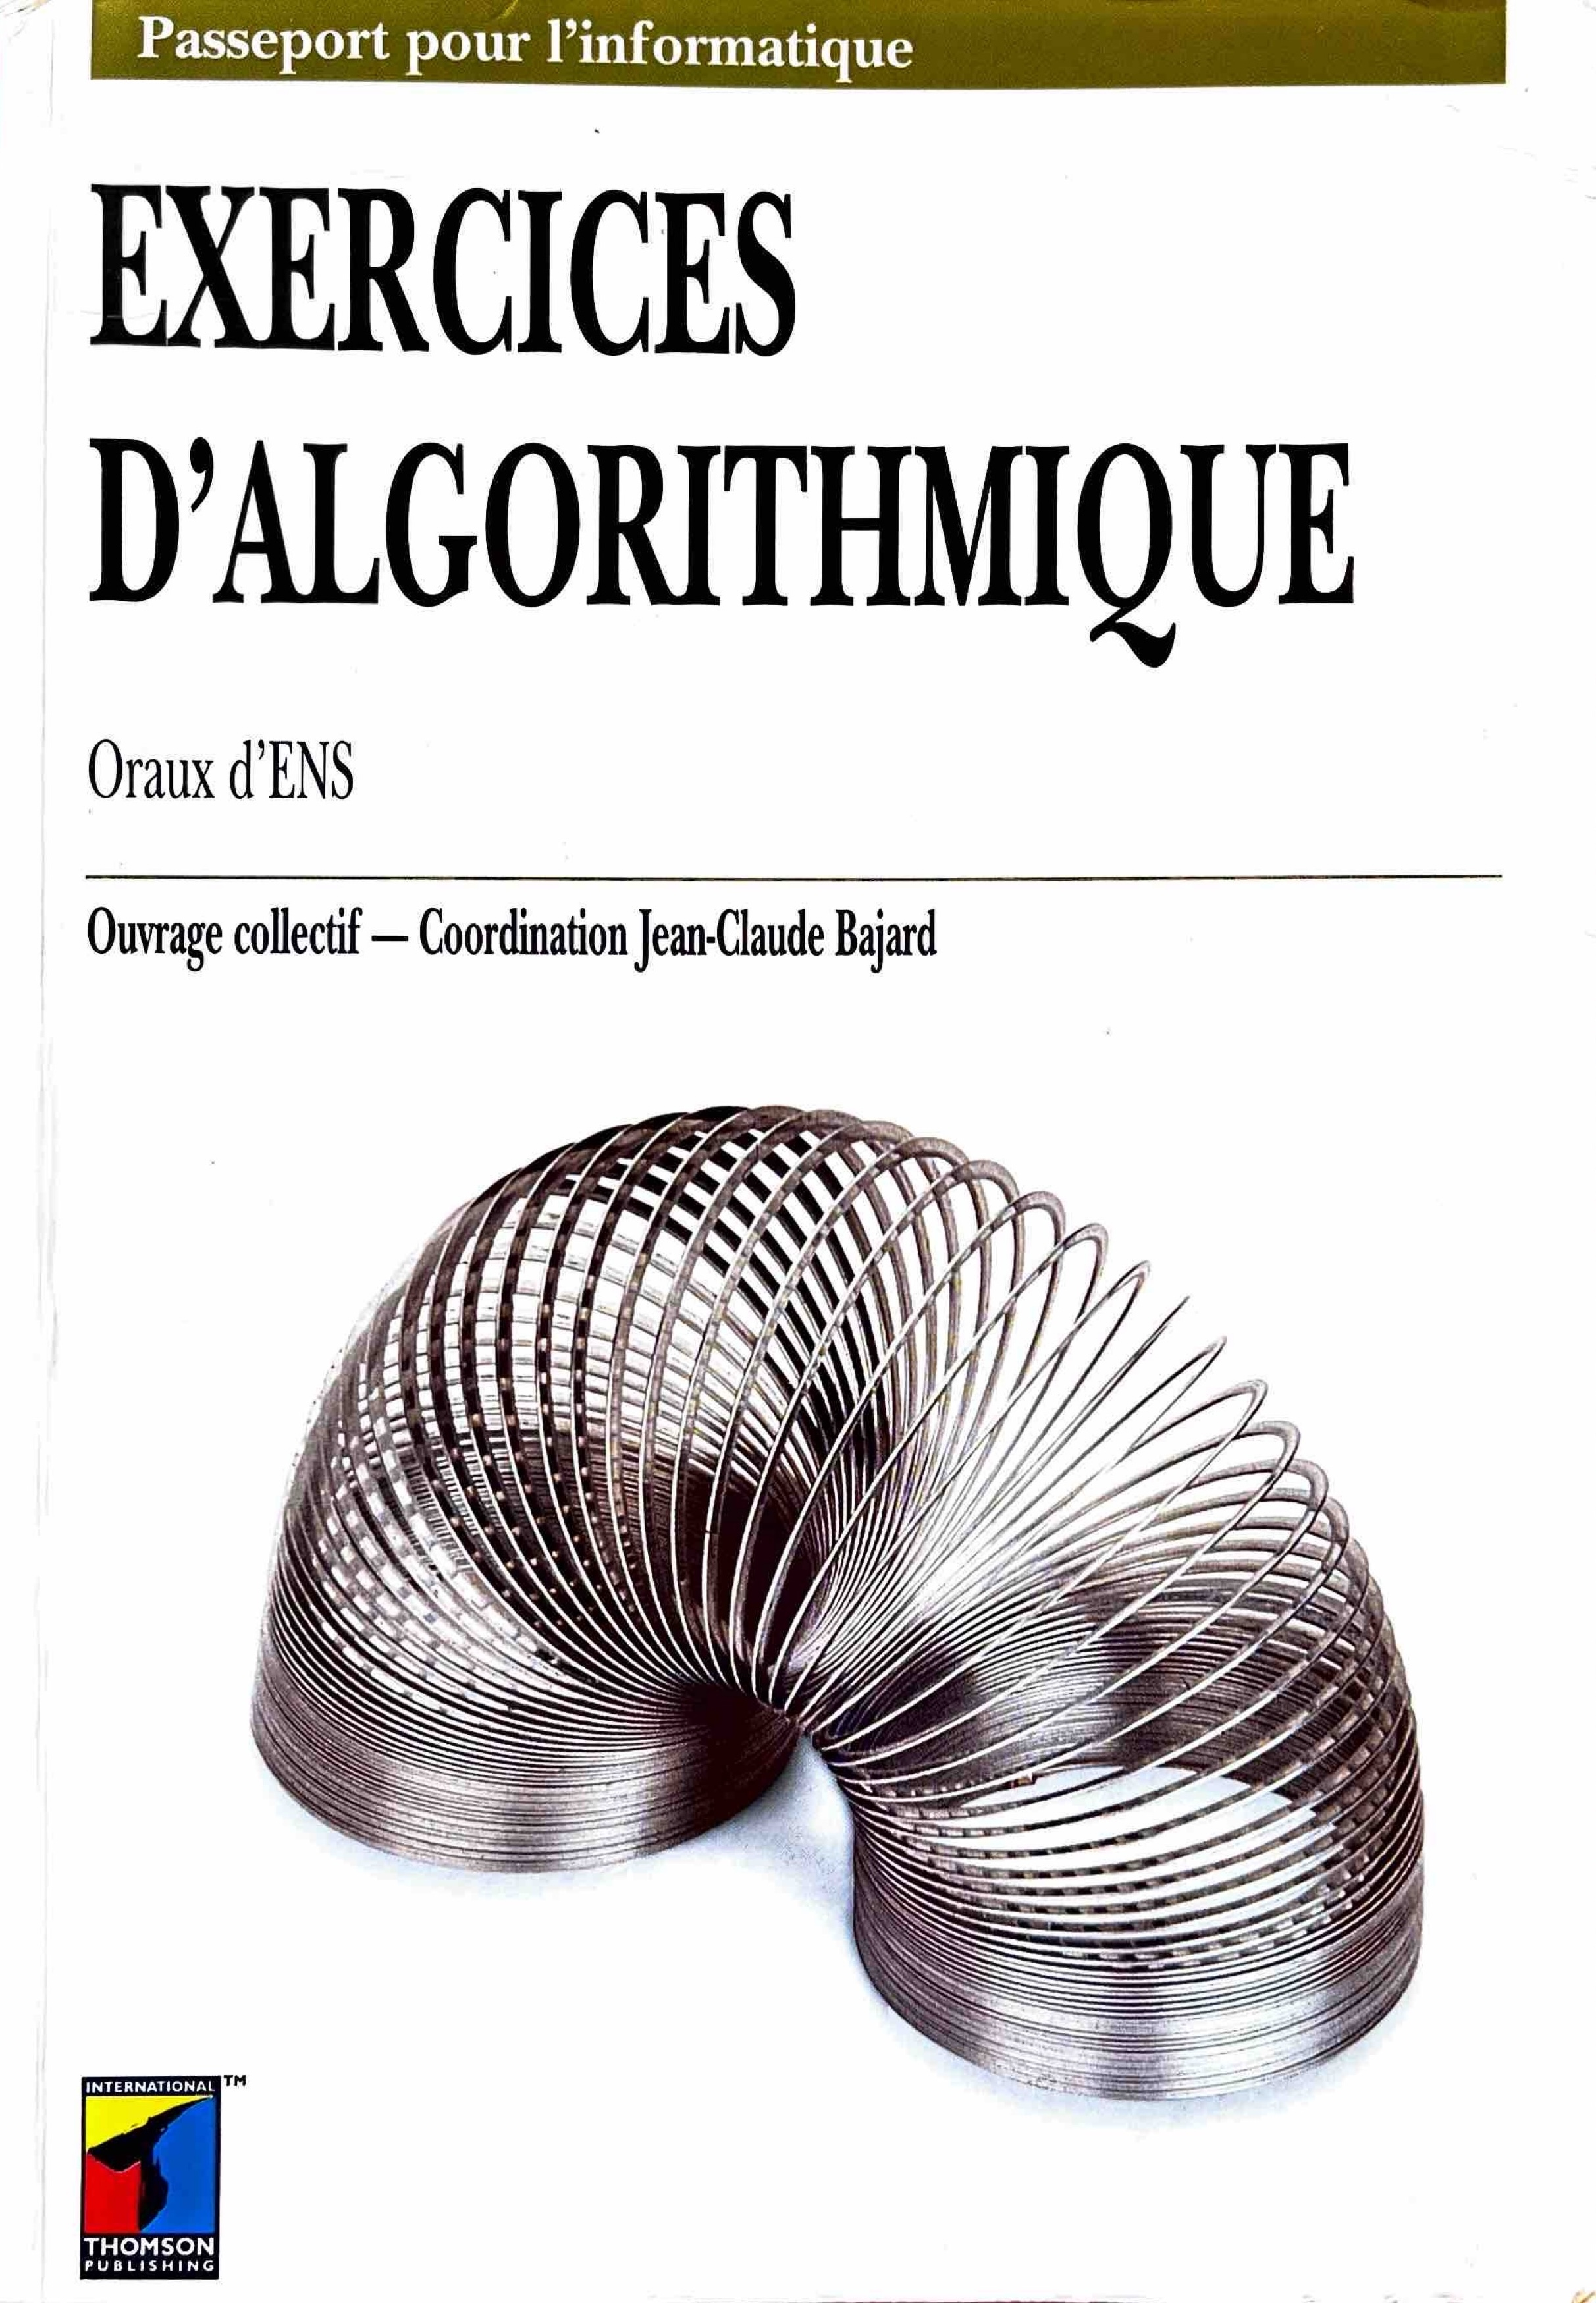
\includepdf{cover}

    % \tableofcontents

    % \chapter{Préface}

Les exercices de cet ouvrage ont été proposés aux oraux des concours d'entrée des Écoles Normales Supérieures de Lyon et de la rue d'Ulm en 1994, 1995 et 1996. Beaucoup sont donnés dans leur forme originelle, d'autres ont été légèrement modifiés pour être un peu plus attractifs et accessibles.
\medskip

Ces exercices étaient généralement précédés de l'avertissement suivant :
\medskip

\textit{\og \ Le but de cet épreuve est de déterminer votre aptitude à\\
    - mettre en forme et analyser un problème\\
    - maîtriser les méthodes logiques propres à l'informatique\\
    - organiser et traiter des informations\\
    - rechercher, concevoir et mettre en forme un ou des algorithmes\\
    - construire méthodiquement un ou des programmes clairs\\
    - exposer de manière synthétique, claire et concise votre travail.}

\medskip
\textit{Le texte de l'épreuve est relativement succinct. Il vous est demandé, suivant votre convenance, de le compléter, pour décrire aussi précisément que possible, les limites d'utilisation de vos algorithmes et programmes. \fg{}}
\medskip

Les exercices sont regroupés par thème. L'étudiant pourra ainsi découvrir les grandes classes d'algorithmes et l'enseignant pourra trouver facilement des exemples pour illustrer un cours ou des travaux dirigés.
\medskip

Mis à part ceux de la rue d'Ulm, les exercices sont proposés avec un corrigé qui ne se veut pas un modèle du genre, qui propose une solution à une question posée. Les algorithmes proposés dans les corrigés sont écrits en OCaml mais aucun exercice n'est dépendant de ce langage de programmation ; ils peuvent tous facilement être retranscrits dans un autre langage. De plus, les parties en OCaml ont juste la prétention d'offrir une mise en forme lisible et rigoureuse des algorithmes proposés. Les fonctions proposées ne sont pas toujours orthodoxes, en particulier pour éviter certaines lourdeurs pouvant rendre la lecture difficile.
\newpage

Cet ouvrage est destiné à un public que l'on souhaite le plus large possible. Tout étudiant de classe préparatoire ou d'université désireux de s'exercer à l'algorithmique devrait y trouver satisfaction.
\medskip

Les auteurs.
\bigskip

\Fin


    \mainmatter

    % \chapter*{Exercices corrigés}
    % \addcontentsline{toc}{chapter}{Exercices corrigés}

    % \chapter{Parcours de tableaux}
    % \Epigraph{Ordre, Permutations, Jeux.}

    % \section{Jeu d'échecs}

Sur un échiquier, on représentera chaque case par ses coordonnées $(i, j)$, la case en bas à gauche étant de coordonnées $(0, 0)$. Sur un tel échiquier, en un coup, un cavalier peut se déplacer de la case $(i, j)$ vers celles d'entre les 8 positions suivantes qui correspondent effectivement à une case de l'échiquier (abscisse et ordonnée comprises entre 0 et 7) : $(i-2, j+1)$, $(i-1, j+2)$, $(i+1, j+2)$, $(i+2, j+1)$, $(i+2, j -1)$, $(i+1, j-2)$, $(i-1, j-2)$ et $(i-2,j-1)$.

\Q
Écrire une fonction OCaml qui donne toutes les cases accessibles en $p$ coups au plus à partir d'une case $(i_0, j_0)$.

\Q
Écrire une fonction OCaml qui indique si toutes les cases sont accessibles à partir d'une case $(i_0, j_0)$ donnée, et si oui, quel est le plus petit nombre de coups permettant d'atteindre à partir de cette case n'importe quelle autre case de l'échiquier.

\Corrige

\Q
Choisissions déjà la structure de données. Définissions un type\\

\texttt{type case = array[1..2] of integer}

Lorem ipsum dolor sit amet consectetur adipiscing elit

\Fin
    % \section{Médiane d'un tableau}

On dispose d'un tableau $A$ de $n$ entiers distincts.

\Q
Écrire une fonction OCaml \texttt{echange (A:int array) (i:int) (j:int) : unit} qui échange les éléments d'indices $i$ et $j$ du tableau $A$.

\Q
Soient $g$ et $d$ deux entiers, $1\leq g\leq d \leq n$. Posons $\alpha=A[g]$. On désire effectuer une permutation des éléments de $A$ d'indice compris entre $g$ et $d$, qui soit telle qu'après la permutation il existe un entier $pivot$, $(g\leq pivot \leq d)$ vérifiant :

\begin{itemize}
    \item $A[\textit{pivot}]=\alpha$,
    \item pour tout $i$ conmpris entre $g$ et \textit{pivot}, $A[i]\leq\alpha$,
    \item pour tout $i$ conmpris entre $\textit{pivot}+1$ et $d$, $A[i]>\alpha$,
    \item les éléments de $A$ d'indice strictement inférieur à $g$ ou strictement supérieur à $d$ restent inchangés.
\end{itemize}

Par exemple, si $n=6$, si les éléments de $A$ sont 5, 8, 7, 3, 9, 15, si $g=2$ et $d=5$, les éléments de $A$ après la permutation seront 5, 3, 7, 8, 9, 15 ou 5, 7, 3, 8, 15, 9, ou... (il n'y a pas unicité des permutations possibles), et \textit{pivot} sera égal à 4. Écrire une fonction OCaml qui effectue la permutation et donne la valeur de \textit{pivot} sans utiliser un autre tableau que $A$. Combien d'affectations (c'est à dire d'instructions \og \texttt{<-} \fg) et de tests nécessite-t-elle?

\Q
On appelle \textit{médiane} de $A$ un couple $(i,\alpha)$ tel que $1\leq i\leq n$, $A[i]=\alpha$, et $E(n/2)$ éléments de $A$ sont inférieurs strictement à $\alpha$ ($E(x)$ est la partie entière de $x$). Proposer une fonction de calcul de la médiane de $A$ utilisant la fonction de la question 2.

\Corrige
\Q
La question 1 est élémentaire.

\Q
Pour la fonction donnant la permutation (c'est une fonction dite de \textit{partition}), on maintient deux indices $i$ et $j$ tels qu'à tout moment les éléments d'indice compris entre $g$ et $i$ sont tous inférieurs ou égaux à $\alpha$, tandis que les éléments d'indice compris entre $j$ et $d$ sont tous supérieurs ou égaux à $\alpha$.
    % \renewcommand{\SourceFile}{1-parcours-de-tableaux/src/1-3.ml}

\vspace{16pt}
\section{Travail sur des tableaux}

On se donne un tableau $T$ d'entiers de taille $N$.

\Q
On se donne un entier $p<N$ et un entier $s$, et on recherche dans le tableau $T$ les indices $k$ tels que $\sum^{p+k}_{i=k}T[i]\geq s$. Écrire une fonction OCaml qui effectue cette recherche. Donner en fonction de $N$ et $p$ un ordre de grandeur du nombre de tests et d'opérations arithmétiques effectuées lors de l'exécution de votre fonction. Pouvez-vous l'améliorer ?

\Q
On suppose maintenant que $T[0] < T[1] < T[2] < ... < T[N-1]$. Pouvez-vous tenir compte de cette information pour obtenir une fonction plus rapide ?

\Q
Proposer une fonction qui affiche les triplets d'entiers $i,j,k$ avec $j<i<N$ tels que $i^2+j^2=k^2$. Pouvez-vous l'améliorer ?

\Corrige

\Q
Première idée : une fonction intuitive, mais quelque peu idiote

\lstinputlisting[linerange={1-10}]{\SourceFile}

Si on réalise que lorsque l'on passe de l'étape $k$ à l'étape $k+1$ dans l'algorithme précédent, deux termes seulement de la somme changent, on obtient la fonction suivante, plus rapide si $p$ est plus grand que 2.

\lstinputlisting[linerange={12-24}]{\SourceFile}

\Q
L'idée est bien sûr de procéder par dichotomie pour savoir à partir de quel rang on a $\sum^{p+k}_{i=k}T[i]\geq s$. On peut procéder comme suit :

\lstinputlisting[linerange={33-43}]{\SourceFile}

Plusieurs variantes permettant de faire moins d'additions en utilisant le \og truc \fg{} de la question 1 sont possibles.

\newpage

\Q
La première idée (idiote!) est de faire une boucle sur $i$, $j$ et $k$ en utilisant le fait que $i^2 < k^2=i^2+j^2 < 2\times i^2$ donc $i < k < \sqrt{2}\times i < 1,5\times i$ d'où $i+1 \leq k \leq \lfloor 1,5\times i \rfloor$ :

\lstinputlisting[linerange={45-55}]{\SourceFile}

on peut ensuite se dire que le seul $k$ qui a une chance de convenir est $\sqrt{i^2+j^2}$ (si c'est un entier !), ce qui donne :

\lstinputlisting[firstline=57]{\SourceFile}

\Fin

    % \renewcommand{\SourceFile}{1-parcours-de-tableaux/src/1-4.ml}

\vspace{16pt}
\section{Deuxième plus grand élément}

Soit $T$ un tableau unidimensionnel d'entiers de taille $n\geq 1$. On cherche à déterminer l'indice du deuxième plus grand élément de $T$ (celui qui viendrait en deuxième position si on rangeait les éléments de $T$ par ordre décroissant).

\Q
Écrire une fonction OCaml qui calcule l'indice du deuxième plus grand élément de $T$ en parcourant une fois le tableau $T$.\\
QUel nombre de comparaisons entre éléments du tableau effectue votre fonction ?

\Q
Pour imaginer une meilleure solution, penser à un tournoi de tennis. Le deuxième meilleur joueur n'est pas forcément le finaliste mais figure parmi les adversaires du gagnant. Pourquoi ?\\
Donner un algorithme qui utilise cette analogie, et déterminer le nombre de comparaisons entre élémentts du tableau qu'il effectue.\\
Écrire alors la fonction OCaml correspondante.

\Corrige

\Q
Première solution évidente :

\lstinputlisting[linerange={1-11}]{\SourceFile}

Les $n-2$ comparaisons \texttt{t.(i) > !max\_1} sont toujours effectuées. Les $n-2$ comparaisons \texttt{t.(i) > !max\_2} le sont aussi dans le pire cas d'un tableau décroissant. Avec les comparaisons implicites de \texttt{min} et \texttt{max} (une seule suffirait mais serait moins lisible), on arrive à $2n-3$, ce qui est intuitif : il faut $n-1$ comparaisons pour trouver le plus grand parmi $n$ (chacun sauf le plus grand doit avoir été comparé à plus grand que lui) et $n-2$ pour trouver le plus grand parmi les $n-1$ éléments restants (même argument).

\Q
C'est clair : tout autre joueur que le gagnant et ses adversaires malheureux est de classement $\geq 3$ puisqu'on connaît deux meilleurs joueurs que lui.
\medskip

Pour l'algorithme, on simule un tournoi de tennis. On transforme les éléments du tableau en feuilles puis on les fusionne en mettant l'indice du plus grand élément des deux à la racine. En itérant jusqu'à n'obtenir qu'un seul arbre, on crée effectivement un arbre de tournoi dont l'indice du vainqueur est la racine.
\medskip

On effectuera $n-1$ comparaisons pour trouver le gagnant (maximum) car chaque match élimine un joueur. On cherche alors le maximum parmi les $\lceil \log_2 n \rceil$ joueurs battus par le gagnant.
\medskip

On commence par définir un type d'arbre et une fonction utilitaire :

\lstinputlisting[linerange={13-16}]{\SourceFile}

\lstinputlisting[firstline=18]{\SourceFile}

\Fin

    % \renewcommand{\SourceFile}{1-parcours-de-tableaux/src/1-5.ml}

\section{Tri d'un petit nombre d'éléments}

Soit $n$ un entier $\geq 2$. Le but de cet exercice est d'étudier les algorithmes de tri d'un tableau de n éléments entiers, pour $n=3,4,5$ et 10. On ne compte que les comparaisons entre éléments du tableau, et on note $Comp(n)$ leur nombre.

\Q
Donner un algorithme, et écrire la fonction OCaml correspondante, pour trier un tableau de taille $n=3$ avec $Comp(n)=3$.\\
Même question avec $n=4$ et $Comp(n)=5$.\\
Même question avec $n=5$ et $Comp(n)=7$.

\Q
On suppose que $n=10$. On demande de préciser le nombre de comparaisons pour chacun des deux algorithmes basés sur les principes suivants (mais on ne demande aucune fonction OCaml dans cette question) :
\medskip

Algorithme 1. Faire deux listes de 5 éléments, utiliser deux fois l'algorithme précédent pour $n=5$ et fusionner les deux listes triées obtenues.
\medskip

Algorithme 2. Faire 5 paires d'éléments et trier les 5 plus grands de chaque paire à l'aide de l'algorithme pour $n=5$. Puis insérer les éléments restants dans la liste formée.

\Corrige
\vspace{.6cm}

Commençons par définir une fonction qui range dans l'ordre deux éléments d'un tableau \texttt{t} en positions \texttt{i} et \texttt{j} :

\lstinputlisting[linerange={1-6}]{\SourceFile}

\Q
Très facile avec 3 éléments : on met le plus petit élément en position 1 en le comparant aux deux autres, puis on classe les deux éléments restants :

\lstinputlisting[linerange={8-11}]{\SourceFile}

Pour 4 éléments : on classe les paires en position (1, 2) et (3, 4), puis on met les deux plus petits en position 1 et le plus grand des deux plus grands en position 4. Enfin, reste à classer les éléments en positions 2 et 3 :

\lstinputlisting[linerange={13-18}]{\SourceFile}

Une autre solution est de trier les 3 premiers éléments (3 comparaisons) puis d'insérer le quatrième, ce qui coute 2 comparaisons supplémentaires en procédant par dichotomie, c'est-à-dire en commençant par l'élément du milieu.
\medskip

Avec 5 éléments : trier les 4 premiers éléments puis insérer le cinquième par dichotomie est ici trop coûteux : il faut 3 comparaisons pour insérer un élément dans une liste de taille 4. Cette solution nous coûterait $5+3=8$ comparaisons.
\medskip

Voici une solution en 7 comparaisons : on prend les 4 premiers éléments, on classe les paires (1, 2) et (3, 4) et on compare les deux plus grands. La situation se résume à l'aide du diagramme :

\begin{center}
    \begin{tikzpicture}[
        label distance=2pt,
        every node/.style={
            font=\ttfamily,
            draw,
            fill=black,
            circle,
            inner sep=0pt,
            minimum size=8pt}]
        \node[label=right:a] (A) at (1,2) {};
        \node[label=right:b] (B) at (2,1) {};
        \node[label=right:c] (C) at (2,0) {};
        \node[label=left:d] (D) at (1,1) {};
        \node[label=right:e] (E) at (4,1) {};

        \draw (A) -- (D);
        \draw (A) -- (B);
        \draw (B) -- (C);
    \end{tikzpicture}
\end{center}

On insère alors le cinquième élément $e$ dans la chaîne $a,b,c$ de longueur 3, ce qui coûte 2 comparaisons. Enfin, on insère le quatrième élément $d$ parmi les éléments inférieurs à $a$ dans l'ensemble $a,b,c,e$ ordonné, ce qui coûte deux comparaisons.

\textbf{TODO: Algorithme}

\Q
Pour l'algorithme 1, le décompte est facile : on utilise deux fois la fonction \texttt{tri\_5}, ce qui conduit à 14 comparaisons. Reste à fusionner deux listes triées de 5 éléments. Or la fusion de deux listes triées de tailles respectives $m$ et $n$ requiert $m+n-1$ comparaisons, soit ici 9 comparaisons. On obtient un total de 23 comparaisons.
\medskip

Pour l'algorithme 2, après les 5 premières comparaisons et la fonction \texttt{tri\_5} appliquée aux 5 plus grands, on a la situation suivante :
\bigskip

\begin{center}
    \begin{tikzpicture}[
        label distance=2pt,
        every node/.style={
            font=\ttfamily,
            draw,
            fill=black,
            circle,
            inner sep=0pt,
            minimum size=8pt}]
        \node[label=right:a] (A) at (.75,4.75) {};
        \node[label=right:b] (B) at (.75,4) {};
        \node[label=right:c] (C) at (.75,3.25) {};
        \node[label=right:d] (D) at (.75,2.5) {};
        \node[label=right:e] (E) at (.75,1.75) {};

        \node[label=left:x] (X) at (0,4) {};
        \node[label=left:y] (Y) at (0,3.25) {};
        \node[label=left:z] (Z) at (0,2.5) {};
        \node[label=left:t] (T) at (0,1.75) {};
        \node[label=left:f] (F) at (0,1) {};


        \draw (A) -- (B);
        \draw (B) -- (C);
        \draw (C) -- (D);
        \draw (D) -- (E);
        \draw (A) -- (X);
        \draw (B) -- (Y);
        \draw (C) -- (Z);
        \draw (D) -- (T);
        \draw (E) -- (F);

    \end{tikzpicture}
\end{center}
\bigskip

Reste à insérer les 4 éléments $x$, $y$, $z$ et $t$ dans la chaîne ordonnée de longueur 6 $f,e,d,c,b,a$. On commence par insérer $z$ dans $d,e,f$ (2 comparaisons) puis on insère $t$ dans la liste qui comprend $f$, $e$ et éventuellement $z$ (encore deux comparaisons). On a :

\begin{center}
    \begin{tikzpicture}[
        label distance=2pt,
        every node/.style={
            font=\ttfamily,
            draw,
            fill=black,
            circle,
            inner sep=0pt,
            minimum size=8pt}]
        \node[label=right:a] (A) at (.75,6.25) {};
        \node[label=right:b] (B) at (.75,5.5) {};
        \node[label=right:c] (C) at (.75,4.75) {};
        \node (S1) at (.75,4) {};
        \node (S2) at (.75,3.25) {};
        \node (S3) at (.75,2.5) {};
        \node (S4) at (.75,1.75) {};
        \node (S5) at (.75,1) {};

        \node[label=left:x] (X) at (0,5.5) {};
        \node[label=left:y] (Y) at (0,4.75) {};


        \draw (A) -- (B);
        \draw (B) -- (C);
        \draw (C) -- (S1);
        \draw (S1) -- (S2);
        \draw (S2) -- (S3);
        \draw (S3) -- (S4);
        \draw (S4) -- (S5);

        \draw (A) -- (X);
        \draw (B) -- (Y);

    \end{tikzpicture}
\end{center}
\bigskip

Insérer $x$ dans la chaîne de longueur 7 dont le plus grand élément est b requiert 3 comparaisons. Enfin, insérer $y$ dans une chaîne de longueur au plus 7 (longueur 6 si $x>b$, longueur 7 sinon) requiert également 3 comparaisons.
\medskip

Le nombre final de comparaisons est donc $5+7+2+2+3+3=22=Comp(10)$.
\medskip

Il se trouve que l'algorithme 2 est optimal. Bien sûr, c'est difficile à prouver ! D'une manière générale, la fonction $Comp\_min(n)$ qui donne le nombre minimal de comparaisons nécessaires pour trier $n$ éléments est très mal connue : on ne connait pas d'expression exacte, juste un équivalent asymptotique en $O(n\log_2n)$.
\bigskip

\Fin

    % \renewcommand{\SourceFile}{1-parcours-de-tableaux/src/1-6.ml}

\section{Représentation de permutations}

On dit qu'une permutation $p$ des entiers 0, 1, ..., $n$ est représentée sous forme normale si elle est stockée dans un tableau \texttt{p} tel que \texttt{p.(i)} contienne l'image de \texttt{i} par la permutation.

\Q
Écrire une fonction qui prend comme entrée une permutation $p$ sous forme normale et calcule le nombre de points fixes de $p$.

\Q
Écrire une fonction qui prend comme entrée une permutation $p$ sous forme normale et calcule le nombre de cycles de $p$.

\Q
On dit qu'une permutation est stockée sous forme de cycles si elle est stockée dans un tableau \texttt{c} construit comme suit : on stocke la permutation cycle par cycle, on regarde le plus petit élément de chaque cycle, on ordonne les cycles par ordre décroissant de leur plus petit élément. Par exemple, la permutation :

\begin{center}
    \begin{tabular}{ |c|c|c|c|c|c|c|c|c| }
        \hline
        i & 0 & 1 & 2 & 3 & 4 & 5 & 6 & 7 \\
        \hline
        \texttt{p.(i)} & 6 & 1 & 0 & 7 & 3 & 4 & 2 & 5 \\
        \hline
       \end{tabular}
\end{center}

a trois cycles, l'un réduit à 1, qui est un point fixe, l'autre de longueur 3, avec 0 qui a pour image 6 qui a pour image 2 qui a pour image 0, et le troisième de longueur 4, avec 4 qui a pour image 3 qui a pour image 7 qui a pour image 5 qui a pour image 4. Les plus petits éléments de ces cycles sont respectivement 1, 0 et 3. En écrivant d'abord le cycle qui contient 3, puis celui qui contient 1, puis celui qui contient 0, on obtient le tableau \texttt{c} :

\begin{center}
    \begin{tabular}{ |c|c|c|c|c|c|c|c|c| }
        \hline
        i & 0 & 1 & 2 & 3 & 4 & 5 & 6 & 7 \\
        \hline
        \texttt{c.(i)} & 3 & 7 & 5 & 4 & 1 & 0 & 6 & 2 \\
        \hline
       \end{tabular}
\end{center}

Écrire une fonction qui construit \texttt{c} à partir de \texttt{p}.

\Q
Montrer que l'application qui a un tableau \texttt{p} associe le tableau \texttt{c} est bijective. Proposer un algorithme qui prend comme entrée une permutation sous forme de cycles et donne en sortie la même permutation représentée sous forme normale. Écrire la fonction correspondante.

\Corrige

\Q
Fonction élémentaire.

\lstinputlisting[linerange={1-4}]{\SourceFile}

\Q
On peut par exemple parcourir les cycles un à un, en marquant les nombres comme \og vus \fg{} au fur et à mesure ; on repère qu'un cycle se termine lorsqu'on retombe sur le premier élément du cycle courant. Pour trouver le cycle suivant, on cherche simplement un nombre qui n'a pas encore été vu. La fonction requiert de manipuler deux boucles imbriquées, la boucle intérieure parcourant le cycle et la boucle extérieure allant de cycle en cycle.

\lstinputlisting[linerange={6-22}]{\SourceFile}

\Q
Un algorithme possible est de parcourir les cycles comme dans la question 2, en remplissant en même temps un tableau \og min \fg{} tel que \texttt{min[j]} contienne le plus petit élément du $j$-ième cycle. Puis on fait un deuxième parcours des cycles pour remplir le tableau de sortie : le premier cycle à parcourir sera celui tel que \texttt{min[j]} soit maximal, et ainsi de suite jusqu'à avoir écrit tous les cycles.

\lstinputlisting[linerange={24-64}]{\SourceFile}

\Q
La seule question pour savoir si la transformation de la question 3 est réversible est de décider comment séparer le tableau en cycles : ensuite, chaque cycle est écrit dans l'ordre ($i$, $p(i)$, $p(p(i))$, etc.), donc il est facile de reconstruire $p$. Pour faire la séparation des cycles, il suffit de remarquer que l'ordre dans lequel on a écrit les cycles, chaque cycle commençant par son plus petit élément et les cycles étant écrits dans l'ordre décroissant, assure que dans un tableau \texttt{c} donnant une permutation sous forme de cycles, $j=c(i)$ est le début d'un nouveau cycle si et seulement si $j$ est minimal parmi $c(0)$, $c(1)$, ..., $c(i)$. Donc l'application est bien inversible.
\medskip

La fonction de passage à une forme normale est en fait nettement plus simple que celle de la question 3. Il suffit de parcourir \texttt{c} en gardant en mémoire le minimum des valeurs vues jusqu'à présent, et en remarquant que $p(c(i))=c(i+1)$ sauf en bout de cycle.

\lstinputlisting[firstline=66]{\SourceFile}

\Fin

    % \renewcommand{\SourceFile}{1-parcours-de-tableaux/src/1-7.ml}

\section{Permutations}

On considère un ensemble $E=\{0,...,N-1\}$. On représente une permutation $p$ de $E$ par un tableau \texttt{p} de taille $N$ tel que l'image d'un élément $i$ de $E$ est \texttt{p.(i)}.

\Q
Écrire un algorithme qui, étant donné un tableau \texttt{p}, vérifie que \texttt{p} représente effectivement une permutation de $E$.

\Q
Écrire un algorithme qui décompose une permutation en cycles.

\Q
On ordonne les permutations par ordre lexicographique (l'ordre du dictionnaire). Par exemple, si $N=4$, $0123<0213<1230<2013$. Écrire un algorithme qui associe à chaque permutation \texttt{p} la permutation suivante dans l'ordre lexicographique (quand elle existe). On pourra utiliser le plus grand entier $i$ tel que $p(i)<p(i+1)$.

\Q
Écrire un algorithme qui énumère toutes les permutations de $E$.

\Corrige

\Q
Il serait particulièrement maladroit de tester successivement si tous les nombres de 0 à $N-1$ sont dans \texttt{p}. Une solution simple consiste à marquer les images rencontrées.

\lstinputlisting[linerange={1-6}]{\SourceFile}

\Q
Comme d'habitude, la bonne idée est de procéder comme on le ferait \og à la main \fg{}. On part de 0 et on regarde ses images successives par la permutation en marquant tous les entiers rencontrés. On s'arrête lorsque l'on retombe sur 0. Puis on recommence avec le premier entier non marqué.
\medskip

Exemple : Soit la permutation $\begin{pmatrix}
    0 & 1 & 2 & 3 & 4 & 5 \\
    4 & 1 & 0 & 5 & 2 & 3
\end{pmatrix}$.
On trouve un premier cycle (0~4~2). Le premier élément non marqué est 1, on trouve un second cycle (1). Le premier élément non marqué est 3, on trouve le troisième et dernier cycle (3~5).

\lstinputlisting[linerange={7-23}]{\SourceFile}

\Q
La difficulté est de comprendre comment on calcule le suivant d'une permutation dans l'ordre lexicographique.
\medskip

\begin{tabular}{ l l }
    Exemple : & le suivant de 0 1 3 2 est 0 2 1 3 \\
     & le suivant de 0 2 1 3 est 0 2 3 1 \\
     & le suivant de 1 2 3 0 est 1 3 0 2
\end{tabular}
\medskip

Il faut donc chercher le plus grand entier $i$ tel que $p(i)$, ..., $p(N-1)$ contienne un élément plus grand que $p(i)$. Il est très facile de voir que cela revient à chercher, comme indiqué dans l'énoncé, le plus grand entier $i$ tel que $p(i)<p(i+1)$. Le suivant est alors obtenu en remplaçant $p(i)$ par le plus petit élément qui lui soit supérieur parmi $p.(i+1)$, ..., $p.(N-1)$. On complète la permutation en triant par ordre croissant les éléments restants.
\medskip

Exemple : Pour $p = 0~1~3~2$, le plus grand élément tel que $p(i)<p(i+1)$ est 1. On remplace 1 par le plus petit élément plus grand que 1 parmi 3 et 2, soit 2. On trie les nombres restants (2 et 3) par ordre croissant. On obtient ainsi 0 2 1 3.
\medskip

Pour éviter d'avoir une fonction de tri à écrire, on peut également marquer les éléments rencontrés dans la recherche du plus grand i tel que $p(i)<p(i+1)$.
\medskip

Le programme de calcul de la permutation $q$ suivant dans l'ordre lexicographique une permutation $p$ fixée va suivre la méthode décrite ci-dessus. La fonction \texttt{max\_croit} renvoie le plus grand entier $i$ tel que $p(i)<p(i+1)$ si un tel entier existe, $-1$ sinon.

\lstinputlisting[linerange={25-31}]{\SourceFile}

La fonction \texttt{inf} renvoie le plus petit entier parmi \texttt{p.(k+1)}, ..., \texttt{p.(N-1)} qui est plus grand que \texttt{p.(k)}.

\lstinputlisting[linerange={33-40}]{\SourceFile}

On a finalement la fonction calculant la permutation suivant \texttt{p} :

\lstinputlisting[linerange={42-72}]{\SourceFile}

\Q
Il suffit d'appliquer l'algorithme de la question précédente de manière itérative à partir de la permutation identité.

\lstinputlisting[firstline=74]{\SourceFile}

\Fin


    % \chapter{Jouer avec les mots}
    % \Epigraph{Reconnaissance, Construction, Codage.}

    % \renewcommand{\SourceFile}{2-jouer-avec-les-mots/src/2-1.ml}

\section{Réécriture de mots}

On considère les mots écrits sur l'alphabet \{a, b, A, B\}, tel que $w=$abbaBabAA par exemple. Soit $\varepsilon$ le mot vide. On dit que deux mots $u$ et $v$ sont en relation si on peut réécrire des parties de $u$ de façon à obtenir $v$ après une suite de transformations effectuées en suivant les règles suivantes :

\begin{center}
    \begin{tabular}{ r c l }
        aA & $\rightarrow$ & $\varepsilon$ \\
        Aa & $\rightarrow$ & $\varepsilon$ \\
        $\varepsilon$ & $\rightarrow$ & aA \\
        $\varepsilon$ & $\rightarrow$ & Aa \\
        bB & $\rightarrow$ & $\varepsilon$ \\
        Bb & $\rightarrow$ & $\varepsilon$ \\
        $\varepsilon$ & $\rightarrow$ & bB \\
        $\varepsilon$ & $\rightarrow$ & Bb \\
        aab & $\rightarrow$ & baa \\
        baa & $\rightarrow$ & aab \\
        bba & $\rightarrow$ & abb \\
        abb & $\rightarrow$ & bba \\
    \end{tabular}
\end{center}

Par exemple :
\begin{center}
    \begin{tabular}{ r l }
         & aababaabAAABBB \\
        $\rightarrow$ & aababbaaAAABBBB \\
        $\rightarrow$ & aababbABBB \\
        $\rightarrow$ & aababbABBB \\
        $\rightarrow$ & aabbbaABBB \\
        $\rightarrow$ & aa \\
    \end{tabular}
\end{center}

\Q
Montrer que cette relation est une relation d'équivalence. Montrer que aa et AA commutent avec toutes les lettres.

\Q
Montrer que tout mot $w$ est équivalent à un mot $xyz$ (formé de trois mots $x$, $y$ et $z$ mis bout à bout), où : $x$ est de la forme aa...aa ou AA...AA et de longueur paire, $y$ est de la forme bb...bb ou BB...BB et de longueur paire, $z$ de la forme ababa...bab, ou ba...bab, ou ab...aba, ou ba...ba, c'est-à-dire alterne les lettres a et b, commençant par a ou b et finissant par a ou b. Un mot de la forme $xyz$ est dit canonique.

\Q
Proposer un codage des mots canoniques sous forme de triplets d'entiers.

\Q
Écrire une fonction \texttt{forme3 (w:string) : bool} qui prend en entrée un mot $w$ et teste si $w$ est un mot alternant les lettres a et b, c'est-à-dire de la forme de $z$.

\Q
Écrire une fonction \texttt{ajouter\_a (iu, ju, ku: int * int * int) : (int * int * int)} qui prend en entrée un mot canonique $u$, codé par un triplet \texttt{(iu, ju, ku)}, et donne en sortie le codage \texttt{(iv, jv, kv)} du mot $v=u$a.

\Q
Écrire une fonction \texttt{representant\_canonique (w:string) : (int * int * int)} qui prend pour entrée un mot quelconque $w$ et donne en sortie un triplet \texttt{(i, j, k)} codant un mot canonique équivalent à $w$.

\Corrige

\Q
Réflexivité : il suffit de prendre une suite de transformations réduite à l'ensemble vide.\\
Symétrie : pour chaque règle, la transformation inverse est dans l'ensemble des règles donc toute suite de transformations peut être inversée.\\
Transitivité : évidente.\\
On a donc une relation d'équivalence.
\bigskip

Commutation de aa avec toutes les lettres : aa commute évidemment avec a.\\
aaA $\rightarrow$ a $\rightarrow$ Aaa, donc aa commute avec A.\\
aab $\rightarrow$ baa est une règle, donc aa commute avec b.\\
aaB $\rightarrow$ BbaaB $\rightarrow$ BaabB $\rightarrow$ Baa, donc aa commute avec B.
\bigskip

Commutation de AA avec toutes les lettres : AAa $\rightarrow$ A $\rightarrow$ aAA, donc AA commute avec a.\\
AA commute évidemment avec A.\\
AAb $\rightarrow$ AAbaaAA $\rightarrow$ AAaabAA $\rightarrow$ bAA, donc AA commute avec b.\\
AAB $\rightarrow$ AABaaAA $\rightarrow$ AAaaBAA $\rightarrow$ BAA, donc AA commute avec B.
\medskip

Remarquons que, de façon symétrique, bb et BB commutent également avec toutes les lettres.

\Q
Pour transformer $w$, on commence par bouger toutes les suites de deux lettres consécutives identiques et les mettre au début du mot, les aa et AA précédant les bb et BB, et par simplifier toutes les occurrences de aA, Aa, bB ou Bb. On se retrouve avec un mot commençant par des aa et AA, continuant avec des bb et BB, et se terminant avec un mot qui alterne des a ou A avec des b ou B. On remplace alors chaque A par AAa et chaque B par BBb, puis on ramène les AA et les BB plus au début : on se retrouve avec une suite de aa et de AA, suivie d'une suite de bb et de BB, suivie d'un mot de la forme de $z$. En simplifiant les aaAA, les AAaa, les bbBB et les BBbb, on obtient mot $xyz$ de la forme requise. Notons qu'il n'est pas demandé ici de montrer l'unicité de cette écriture.

\Q
On peut coder $x$ par un entier $i$, positif si x contient des aa et négatif s'il contient des AA, et de valeur absolue égale au nombre de lettres de $x$. De même, $y$ peut être codé par un entier $j$. On peut coder $z$ par un entier $k$, positif si $z$ commence par un a et négatif si $z$ commence par un b, et de valeur absolue égale au nombre de lettres de $z$.

\Q
Supposons la longueur de $w$ supérieure ou égale à 1. On regarde la première lettre de $w$, puis on teste si les suivantes alternes, en s'arrêtant dès qu'on trouve une erreur ou qu'on a parcouru tout le mot.

\lstinputlisting[linerange={1-11}]{\SourceFile}
\newpage

\Q
La fonction n'est pas difficicle mais demande un peu d'attention pour ne pas faire d'étourderie : il est particulièrement recommandé d'écrire d'abord l'algorithme en détail. Si $z$ est non vide et se termine par un b : \texttt{ku} strictement positif et pair ou strictement négatif et impair ; alors $z$ s'allonge d'une lettre : \texttt{ku} augmente de 1 dans le premier cas et diminue de 1 dans le deuxième cas. Si $z$ est non vide et se termine par un a : \texttt{ku} strictement positif et impair ou strictement négatif et pair ; alors $z$ raccourcit d'une lettre et $x$ change : \texttt{ku} diminue de 1 dans le premier cas et augmente de 1 dans le second cas, et \texttt{iu} augmente de 2 s'il était positif et diminue de 2 s'il était strictement négatif. Si $z$ est vide : $\texttt{ku}=0$ ; alors \texttt{ku} devient égal à 1. D'où la fonction suivante :

\lstinputlisting[linerange={13-23}]{\SourceFile}

\Q
On peut supposer qu'on dispose des fonctions \texttt{ajouter\_b}, \texttt{ajouter\_A} et \texttt{ajouter\_B} similaires à celle de la question 5. Il est alors facile d'ajouter des lettres une par une pour construire un mot canonique pour chaque préfixe de $w$ et finalement pour $w$.

\lstinputlisting[linerange={30-39}]{\SourceFile}
\medskip

La relation d'équivalence étudiée dans cet exercice correspond à un groupe donné par une permutation finie : les éléments sont les classes d'équivalence de la relation définie à la question 1, et on peut facilement vérifier que cette relation est compatible avec la concaténation. L'étude faite ici consiste en la construction d'une \og structure automatique \fg{} pour le groupe, permettant de calculer un représentant distingué de la classe du produit de deux éléments donnés. L'étude de groupes automatiques est un domaine de recherche récent et actif en mathématiques.
\bigskip

\Fin

    % \renewcommand{\SourceFile}{2-jouer-avec-les-mots/src/2-2.ml}

\section{Pliage de papier}

On prend une feuille de papier et on la plie $n$ fois dans le sens vertical, en repliant à chaque fois la moitié droite sur la gauche. Les plis de la feuille, une fois redépliée, sont une suite de creux et de bosses. Voir figure :
\medskip

\begin{tikzpicture}[scale=1.1]
    \draw (0,0) rectangle (4,2);

    \node[font=\ttfamily, below=.1cm of {1.2,0}] {étape 0};
\end{tikzpicture}\hspace{2cm}
\begin{tikzpicture}[scale=1.1]
    \draw (0,0) rectangle (4,2);
    \draw (2,0) -- (2,2);

    \node[font=\ttfamily, below=.1cm of {1.2,0}] {étape 1};
\end{tikzpicture}
\medskip

\begin{tikzpicture}[scale=1.1]
    \draw (0,0) rectangle (4,2);
    \draw (1,0) -- (1,2);
    \draw (2,0) -- (2,2);
    \draw[ultra thick] (3,0) -- (3,2);

    \node[font=\ttfamily, below=.1cm of {1.2,0}] {étape 2};
\end{tikzpicture}\hspace{2cm}
\begin{tikzpicture}[scale=1.1]
    \draw (0,0) rectangle (4,2);
    \draw (.5,0) -- (.5,2);
    \draw (1,0) -- (1,2);
    \draw [ultra thick](1.5,0) -- (1.5,2);
    \draw (2,0) -- (2,2);
    \draw (2.5,0) -- (2.5,2);
    \draw[ultra thick] (3,0) -- (3,2);
    \draw[ultra thick] (3.5,0) -- (3.5,2);

    \node[font=\ttfamily, below=.1cm of {1.2,0}] {étape 3};
\end{tikzpicture}
\vspace{.4cm}

\hspace{.6cm}
\begin{tikzpicture}
    \draw (0,0) -- (0,.6);
    \node[font=\ttfamily, right=.2cm of {0,.3}] {$\leftarrow$ creux};

    \draw[ultra thick] (4,0) -- (4,.6);
    \node[font=\ttfamily, right=.2cm of {4,.3}] {$\leftarrow$ bosse};
\end{tikzpicture}

\Q
Combien y a-t-il de plis à la n-ième étape ?

\Q
On représente chaque étape du pliage par un mot. Un creu est codé par un 0 et une bosse par un 1. Ainsi : $w_0=\varepsilon$ (mot vide)\\
$w_1=0$\\
$w_2=001$\\
$w_3=0010011$\\
\dots
\medskip

Montrer que $w_i$ est toujours un préfixe de $w_{i+1}$, c'est à dire que le début de $w_{i+1}$ coïncide avec $w_i$.

\Q
Donner un algorithme de construction de $w_n$ à partir de $w_{n-1}$. Écrire une fonction de calcul de $w_n$. On prendra comme entrée $n$ et on renverra une liste \texttt{w} d'entiers remplie adéquatement.

\Q
Écrire une fonction qui prend pour entrée un entier $n$ et renvoie une liste contenant la représentation binaire de $n$, poids fort en tête.

\Q
Les mots de la suite de pliage étant préfixes les uns des autres, on peut considérer le mot infini $w$ dont ils sont tous préfixes. Proposer un algorithme qui prend pour entrée la représentation binaire de $n$ et renvoie le $n$-ième bit de $w$.

\Corrige

\Q
Si on considère les intervalles entre les plis (y compris les côtés de la feuille), on a 1 intervalle, puis 2, puis 4, etc. ; à chaque étape, chaque intervalle est coupé en deux et le nombre d'intervalles double. Après $n$ étapes, il y a donc $2^n$ intervalles, et le nombre de plis est $2^n-1$.

\Q
Déchirons le papier le long du pli de la première étape et débarrassons-nous de la moitié de droite : la $k$-ième étape de pliage du papier initial est comme la $(k-1)$-ième étape de pliage du demi-papier, et donc $w_{k-1}$ forme la moitié gauche de $w_k$.

\Q
Le pli du milieu est un creux et donc donne un 0 au milieu de $w_n$. Le demi-papier droit est plié, après la première étape, comme le demi-papier gauche, sauf qu'il est tourné dans l'autre sens. Soit $\textrm{r}(w)$ le mot obtenu à partir d'un mot $w$ en lisant les chiffres de droite à gauche, et $\textrm{c(w)}$ le mot obtenu à partir de $w$ en remplaçant chaque 0 par un 1 et chaque 1 par un 0 : on a la relation de récurrence
\[
    w_n = w_{n-1}\,0\,\textrm{c}(\textrm{r}(w_{n-1}))
\]
De cette relation, se déduit facilement la fonction permettant de construire $w_n$.

\lstinputlisting[linerange={1-5}]{\SourceFile}

\Q
Question classique et accessible à tous.

\lstinputlisting[linerange={7-12}]{\SourceFile}

\Q
On peut trouver un autre point de vue pour construire $w_k$ par récurrence à partir de $w_{k-1}$ : on intercale un nouveau pli entre chaque paire de plis consécutifs de $w_{k-1}$, et ce pli est alternativement 0 ou 1, le premier étant 0. Ainsi : $w_k=0x1x0x...x1$, si $w_{k-1}=xxx...xx$. Donc le $n$-ième bit de $w$ est facile à trouver si $n$ est impair : c'est 0 si $n$ est congru à 1 modulo 4 et c'est 1 si $n$ est congru à 3 modulo 4. Si $n$ est pair, on divise $n$ par deux et on remarque que le $n$-ième bit de $w_k$ est le $(n/2)$-ième bit de $w_{k-1}$, donc si $n/2$ est impair, il suffit encore une fois de tester si $n/2$ est congru à 1 ou à 3 modulo 4. Si $n/2$ est est pair, on redivise par deux, et ainsi de suite. Lorsque $n$ est écrit en binaire, on regarde son bit le plus à droite (celui de poids le plus faible), puis le bit immédiatement à sa gauche, et ainsi de suite jusqu'à trouver un bit égal à 1. Soit $x$ le $n$-ième bit de $w$. On a :\\
Si $n=1~0~0~...~0$, alors $x=0$.\\
Si $n=*~*~...~*~0~1~0~0~...~0$, alors $x=0$.\\
Si $n=*~*~...~*~1~1~0~0~...~0$, alors $x=1$.\\
Car un nombre se terminant par 0~1 est congru à 1 modulo 4 et un nombre se terminant par 1~1 à 3 modulo 4.
Ceci donne un programme extrêmement simple.

\lstinputlisting[firstline=14]{\SourceFile}
\medskip

Des études du genre de celle faite dans cet exercice peuvent servir à montrer des propriétés d'algébricité ou de transcendance du nombre étudié. C'est actuellement un domaine actif de recherche en France. On obtient une suite de courbes $(C_n)$ approximant une courbe de Peano (c'est-à-dire une courbe qui remplit le plan), définie à partir de $(w_n)$, en dessinant un segment de longueur $1/2^{n/2}$ pour chaque bit lu, et en tournant à droite (de $+\pi/2$) ou à gauche (de $-\pi/2$) à chaque pas, selon que le bit lu est 0 ou 1. Le premier segment est dessiné dans la direction $\pi/4$. La figure suivante illustre les premiers pas :

\begin{center}
\begin{tikzpicture}[scale=.8]
    \draw (0,0) -- (3,0);

    \node[font=\ttfamily, above=.1cm of {1.2,0}] {C0};
\end{tikzpicture}\hspace{2cm}
\begin{tikzpicture}[rotate=45, scale=.8]
    \draw (0,2.1) -- (2.1,2.1);
    \draw (2.1,2.1) -- (2.1,0);

    \node[font=\ttfamily, below=.1cm of {1.6,1.4}] {C1};
\end{tikzpicture}
\vspace{1cm}

\begin{tikzpicture}[scale=.8]
    \draw (0,0) -- (0,1.5);
    \draw (0,1.5) -- (1.5,1.5);
    \draw (1.5,1.5) -- (1.5,0);
    \draw (1.5,0) -- (3,0);

    \node[font=\ttfamily, above=.1cm of {1,0}] {C2};
\end{tikzpicture}\hspace{2cm}
\begin{tikzpicture}[rotate=45, scale=.8]
    \draw (0,2.2) -- (0,3.3);
    \draw (0,3.3) -- (1.1,3.3);
    \draw (1.1,3.3) -- (1.1,2.2);
    \draw (1.1,2.2) -- (2.2,2.2);
    \draw (2.2,2.2) -- (2.2,1.1);
    \draw (2.2,1.1) -- (1.1,1.1);
    \draw (1.1,1.1) -- (1.1,0);
    \draw (1.1,0) -- (2.2,0);

    \node[font=\ttfamily, below=.1cm of {.9,2}] {C3};
\end{tikzpicture}
\end{center}
\medskip

\Fin

    % \renewcommand{\SourceFile}{2-jouer-avec-les-mots/src/2-3.ml}

\section{Plus longue sous-suite croissante}

Une suite finie d'entiers $(a_i)_{1\leq i \leq n}$ est représentée par un tableau d'entiers \texttt{a} en OCaml.
\medskip

On cherche la longueur de la (ou les) plus longue(s) sous-suite(s) croissante(s) (au sens large) de la suite d'entiers. Par exemple, si $n=9$, et si les termes de la suite sont 1, 2, 6, 4, 5, 11, 9, 12, 9, la longueur cherchée est 6, et elle est atteinte par les sous-suites croissantes :
\begin{itemize}
    \item 1, 2, 4, 5, 11, 12
    \item 1, 2, 4, 5, 9, 12
    \item 1, 2, 4, 5, 9, 9
\end{itemize}

\Q
Écrire une fonction donnant la longueur de la plus longue sous-suite croissante de la suite \texttt{a}. Estimer le nombre de comparaisons que demande votre fonction. Pourriez-vous l'améliorer ?

\Q
Modifiez votre fonction de manière à pouvoir afficher la plus longue (ou une des plus longues s'il y en a plusieurs de longueur maximale) sous-suites croissantes de \texttt{a}.

\Corrige

\Q
Il suffit de procéder par étapes, en ajoutant les éléments de \texttt{a} au fur et à mesure. Définissons un tableau \texttt{l} tel que \texttt{l.(p)} est la longueur de la plus longue sous-suite se terminant par \texttt{a.(p)}. Une plus longue sous-suite croissante se terminant par \texttt{a.(p)} est soit formée uniquement de \texttt{a.(p)} si pour tout $i < p$, on a \texttt{a.(i) > a.(p)}, soit obtenue en ajoutant \texttt{a.(p)} à la plus longue des plus longues sous-suites se terminant par un \texttt{a.(i)} tel que $i < p$ et \texttt{a.(i) < a.(p)}. À la fin, il ne reste plus qu'à chercher le plus grand des \texttt{l.(i)}, $1 \leq i \leq n$. Ceci nous donne la fonction suivante :

\lstinputlisting[linerange={1-19}]{\SourceFile}

On fait 2 fois $1 + 2 + ... + (n-1)$, soit $n(n-1)$ tests plus les $n-1$ derniers tests de la dernière boucle \og for \fg{}. Ceci donne $(n+1)(n-1)$ tests. On peut gagner un peu de temps en classant \texttt{l} non par ordre croissant des valeurs de \texttt{p} mais par ordre croissant des valeurs de \texttt{a.(p)} et en simulant une structure dynamique pour insérer un nouvel élément sans devoir tout déplacer. Ce sera un peu lourd !

\Q
On peut dans un premier temps créer un matrice auxiliaire \texttt{s} telle que \texttt{s.(p).(i)} contient le $i$-ième élément d'une plus longue sous-suite croissante se terminant par \texttt{a.(p)} (note : pas besoin d'une \og marque de fin \fg{}, on sait que le dernier élément est \texttt{a.(p)} et on connaît la longueur d'une telle sous-suite, c'est \texttt{l.(p)}). Il est plus malin de remarquer que si l'élément qui précède \texttt{a.(p)} dans une telle sous-suite est \texttt{a.(i)}, alors la sous-suite correspondante s'obtient en ajoutant \texttt{a.(p)} à la plus longue sous-suite qui se termine par \texttt{a.(i)}. Il suffit donc de mémoriser $i$. On obtient alors, en déclarant un tableau \texttt{precedent} :

\lstinputlisting[firstline=21]{\SourceFile}

Cette fonction affichera une plus longue sous-suite à l'envers. L'afficher à l'endroit n'est pas difficile.

\Fin

    % \renewcommand{\SourceFile}{2-jouer-avec-les-mots/src/2-4.ml}

\section{Recherche de motifs}

Un mot $u$ est une suite $(u_1, u_2, ..., u_n)$ de lettres, l'entier $n$ est la longueur du mot $u$. La suite vide correspond au mot vide, noté $\varepsilon$, de longueur 0. La concaténation de deux mots $u=(u_1, u_2, ..., u_n)$ et $v=(v_1, v_2, ..., v_k)$, notée $uv$, est simplement le mot $(u_1, u_2, ..., u_n, v_1, v_2, ..., v_k)$. Il est facile de vérifier que la concaténation est une opération associative pour laquelle le mot vide est élément neutre à gauche et à droite. Le mot $v$ est dit facteur ou motif d'un mot $u$ s'il existe des mots $g$ et $d$ tels que $u=gvd$. Si le mot $g$ (resp. $d$) est la suite vide, on dit que $v$ est un préfixe (resp. suffixe) de $u$.

\Q
Modéliser la situation décrite. Écrire un algorithme qui, étant donnés deux mots $u$ et $v$, vérifie si $v$ est un facteur de $u$. Quel est le nombre maximum de comparaisons effectuées par votre algorithme ?

\Q
Si $v$ n'est pas le mot vide, on note $Bord(v)$ le plus grand mot distinct de $v$ qui soit à la fois préfixe et suffixe de $v$. Par exemple, si $v=abacaba$, $Bord(v)=aba$. Soit $v=(v_1, v_2, ..., v_k)$. Pour tout $i$ entre 1 et $k$, on définit $B(i)$ comme étant la longueur de $Bord(v_1 ... v_k)$.
\smallskip

Utiliser cette fonction $B$ pour écrire un nouvel algorithme vérifiant si un mot $v$ est facteur d'un mot $u$. Quel est le nombre maximum de comparaisons effectuées par ce nouvel algorithme ?

\Q
Soit $v=(v_1, v_2, ..., v_k)$ et $a$ une lettre. On admet que $Bord(va)$ est le plus long préfixe de $v$ qui soit dans $\{\varepsilon, Bord(v)a,Bord^2(v)a, ..., Bord^k(v)a\}$ (en posant $Bord(\varepsilon)=\varepsilon$). Déduire de ce résultat un algorithme qui, étant donné un mot $v=(v_1, v_2, ..., v_k)$, calcule successivement $B(1), ..., B(k)$.

\newpage

\Corrige

\Q
La modélisation suggérée consiste à représenter les mots par des chaînes de caractères.
\medskip

L'algorithme naïf, mais naturel, consiste à comparer $v$ avec les facteurs de $u$ de même longueur que $v$ en commençant en posotion 0, puis 1, 2... jusqu'au succès ou à la fin de $u$.

\lstinputlisting[linerange={1-12}]{\SourceFile}

Chaque appel à la fonction \texttt{String.equal} amène à au plus $k$ comparaisons. Le nombre d'appels à \texttt{String.equal} étant d'au plus $(n-k+1)$, le nombre total de comparaisons effectuées par cet algorithme est au plus $k(n-k+1)$. Le maximum est atteint pour les mots de la forme $u=a^{n-1}b$ et $v=a^{k-1}b$.

\Q
La primitive Caml \texttt{equal} compare les chaînes de caractère passées en argument octet par octet (caractère par caractère). On donne la code OCaml équivalent suivant :

\lstinputlisting[linerange={14-24}]{\SourceFile}

Supposons que l'appel à \texttt{String.equal} renvoie false lors de la comparaison entre $u_{i+j-1}$ et $v_j$. On a alors la situation suivante :
\begin{center}
    \begin{tabular}{ c c c c c }
        $u_i$ & $u_{i+1}$ & ... & $u_{i+j-2}$ & $u_{i+j-1}$ \\
        = & = & & = & $\neq$ \\
        $v_1$ & $v_2$ & ... & $v_{j-1}$ & $v_{j}$
    \end{tabular}
\end{center}

On va donc ensuite comparer la chaîne de caractères $(u_{i+1}, u_{i+2}, ..., u_{i+j})$ à $v$. Pour que cet appel renvoie $true$, il faut en particulier que $v_1=v_2$, ..., $v_{j-2}=v_{j-1}$. Ces égalités signifient exactement que $Bord(v_1...v_{j-1})=v_1...v_{j-2}$. Ainsi, si $Bord(v_1...v_{j-1}) \neq v_1...v_{j-2}$, il est inutile d'appeler \texttt{String.equal} avec la chaîne de caractères $(u_{i+1}$, $u_{i+2}$, ..., $u_{i+j})$. De façon identique, on voit que si $Bord(v_1...v_{j-1}) \neq v_1...v_{j-3}$, l'appel à \texttt{String.equal} avec la chaîne de caractères $(u_{i+2}, u_{i+3}, ..., u_{i+j+1})$ est inutile. En répétant le raisonnement, il apparaît que le premier appel qui ne soit pas voué à l'échec est celui où $u_{i+j-1}$ est comparé à $v_{1+B(j-1)}$. Cette remarque conduit alors au nouvel algorithme suivant, où on suppose la fonction \texttt{b} correspondant à $B$ définie :

\lstinputlisting[linerange={51-64}]{\SourceFile}

Le nombre maximal de comparaisons peut être évalué comme suit. Appelons \og positif \fg{} un test $u_i=v_j$ évalué à $true$ et négatif un test $u_i=v_j$ évalué à $false$. Lors d'un test positif, $i$ augmente, il y a donc au plus $n$ tests positifs. Lors d'un test négatif, la quantité $i-j$ augmente : elle vaut 0 au commencement de l'algorithme et au plus $n$ lorsque l'algorithme se termine. Ainsi, il y a également au plus $n$ tests négatifs. En conclusion, ce second algorithme effectue donc au plus $2n$ comparaisons.

\Q
On a bien sûr $B(1)=0$ et $B(2)=1$ si $v_1=v_2$, 0 sinon.
\smallskip

Supposons calculés $B(1)$, ..., $B(h-1)$. D'après l'indication donnée dans l'énoncé, $B(h)$ est la longueur du plus long préfixe de $v_1...v_h$ qui soit dans
\[
    \{\varepsilon, Bord(v_1...v_{h-1})v_h,Bord^2(v_1...v_{h-1})v_h, ...\}
\]
Il est clair que la longueur des mots $Bord^i(v_1...v_{h-1})v_h$ décroit (au sens large) lorsque $i$ croit. Ainsi, il faut d'abord tester si $Bord(v_1...v_{h-1})v_h$ est un préfixe de $v_1...v_h$, puis si ce n'est pas le cas, si $Bord^2(v_1...v_{h-1})v_h$ est un préfixe de $v_1...v_h$, etc. En remarquant que $Bord(v_1...v_{h-1})v_h$ est un préfixe de $v_1...v_h$ si et seulement si $v_h=v_{1+B(h-1)}$, on est amenés naturellement à l'algorithme suivant, renvoyant le tableau $[B(1), B(2), ..., B(k)]$ :

\lstinputlisting[linerange=26-46]{\SourceFile}

En considérant la quantité $h-j$, on obtient par un argument similaire à celui de la question 2 que le nombre de comparaisons effectuées est au plus $2k$.
\bigskip

L'indication de l'énoncé : $Bord(va)$ est le plus long préfixe de $v$ qui soit dans \newline $\{\varepsilon, Bord(v)a,Bord^2(v)a, ..., Bord^k(v)a\}$ se démontre comme suit.\\
On dit que $w$ est un bord de $v$ si $w$ est à la fois un préfixe et un suffixe de $v$. Soit $z$ un bord de $va$. Si $z \neq \varepsilon$, $z = z'a$, où $z'$ est un bord de $v$. Ou bien $z'=Bord(v)$, ou bien $z'$ est un bord de $Bord(v)$. Par induction, il vient immédiatement que $z'$ est de la forme $Bord^i(v)$ pour un certain $i$ tel que $1 \leq i \leq k$. Ainsi, $z$ est dans l'ensemble $\{\varepsilon, Bord(v)a,Bord^2(v)a, ..., Bord^k(v)a\}$.
\smallskip

Réciproquement, tout mot de cet ensemble est clairement suffixe de $va$, donc un bord de $va$ s'il est préfixe de $va$.
\bigskip

\Fin

    % \renewcommand{\SourceFile}{2-jouer-avec-les-mots/src/2-5.ml}

\section{Mots bien parenthésés}

On considère une parenthèse ouvrante \og ( \fg{} et une parenthèse fermante \og ) \fg{}. Un mot parenthésé $u$ est une suite de parenthèses ouvrantes et fermantes. Le nombre de parenthèses utilisées est appelée la longueur du mot. La suite vide correspond au mot vide, noté $\varepsilon$. La concaténation de deux mots parenthésés $u$ et $v$, notée $uv$, est simplement le mot parenthésé obtenu en mettant $u$ et $v$ bout à bout. Ainsi, si $u=((()()$ et $v=))$, $uv=((()()))$. Un mot parenthésé $v$ est dit facteur gauche d'un mot parenthésé $u$ s'il existe un mot $w$ tel que $u=vw$. Un mot parenthésé $u$ est bien parenthésé s'il contient autant de parenthèses ouvrantes que de parenthèses fermantes et si tout facteur gauche $v$ de $u$ contient au moins autant de parenthèses ouvrantes que de parenthèses fermantes.

\Q
Modéliser la situation décrite et écrire un algorithme qui, étant donné un mot parenthésé, vérifie s'il est bien parenthésé ou non.

\Q
Montrer que, étant donné un mot bien parenthésé non vide $u$, il existe un unique couple $(v, w)$ de mots bien parenthésés tels que $u=(v)w$. Écrire un algorithme qui, étant donné le mot $u$, calcule les mots $v$ et $w$.

\Q
Soit $N\in\mathbb{N}$. Écrire un algorithme qui énumère tous les mots bien parenthésés de longueur au plus $N$.

\Corrige

\Q
Une solution est de modéliser un mot parenthésé par une chaîne de caractères ne contenant que des parenthèses.
\smallskip

Pour tester si un mot $u$ est bien parenthésé, il suffit de vérifier que $u$ contient autant d'ouvrantes que de fermantes et que tout facteur gauche de $u$ contient plus de parenthèses ouvrantes que de fermantes. On peut pour cela gérer un compteur que l'on incrémente (resp. décrémente) lorsque l'on trouve une parenthèse ouvrante (resp. fermante). On suppose ici que $u$ est bien formé (i.e ne contient que des parenthèses).

\lstinputlisting[linerange={1-12}]{\SourceFile}

\Q
Montrons tout d'abord l'unicité de la décomposition proposée. Supposons qu'un mot $u$ se décompose en $u=(v)w=(v')w$ avec $v \neq v'$. Il est clair que si $v$ et $v'$ sont de même longueur alors $v=v'$. Par symétrie, il suffit de traiter le cas où $v'$ est de longueur strictement plus grande que $v$. Ainsi $v'=v)v''$ où $v''$ est un mot parenthésé éventuellement vide. Comme $v$ est bien parenthésé, il contient autant d'ouvrantes que de fermantes. Ainsi, le préfixe $v)$ de $v'$ contient une fermante de plus que d'ouvrantes, ce qui est en contradiction avec le fait que $v'$ soit bien parenthésé. On a ainsi montré l'unicité de la décomposition.
\medskip

Soit $u$ un mot bien parenthésé. Pour montrer l'existence d'une décomposition, considérons le plus petit facteur gauche non vide $u'$ de $u$ qui contienne autant d'ouvrantes que de fermantes ($u'$ existe puisque $u$ a cette propriété). Dans la fonction de la question précédente, $u'$ correspond au plus petit facteur gauche non vide pour lequel la variable \texttt{cpt} prend la valeur 0. Ainsi, il est facile de voir que $u'$ commence par une ouvrante et finit par une fermante : $u'=(v)$. En utilisant le fait que $u$ est bien parenthésé, on vérifie aisément que $v$ et $w$, où $w$ est défini par $u=u'w$, sont bien parenthésés.
\medskip

Le calcul de $v$ et $w$ repose sur le remarque que $(v)$ est le plus petit facteur de $u$ qui contienne autant d'ouvrantes que de fermantes.

\lstinputlisting[linerange={14-29}]{\SourceFile}

\Q
L'idée est bien entendu d'utiliser la question précédente. Si l'on connaît tous les mots bien parenthésés de longueur au plus $L$, où $L$ est une certaine constante, on obtient un mot bien parenthésé de longueur $L+2$ en prenant un mot bien parenthésé $u$ de longueur $k$, un mot bien parenthésé de longueur $L-k$ et en construisant le mot $(u)v$. Il est donc nécessaire de garder en mémoire tous les mots parenthésés déjà construits.
\medskip

Nous allons ici utiliser un tableau de listes tel que la liste à l'indice $i$ contient tous les mots bien parenthésés de longueur $2i$.

\lstinputlisting[firstline=31]{\SourceFile}

Remarque : Le nombre de mots bien parenthésés de longueur $2n$ est égal à $\frac{1}{n+1}\binom{2n}{n}$, le $n$-ième nombre de Catalan.
\bigskip

\Fin

    % \renewcommand{\SourceFile}{2-jouer-avec-les-mots/src/2-6.ml}

\section{Plus longue sous-suite commune}

Notation : Si $X$ est une chaîne de caractères, on désignera par $X_l$ le préfixe de $X$ de longueur $l$.
\medskip

Une sous-suite du mot $A=a_1a_2...a_n$ est un mot obtenu en supprimant certaines lettres. Par exemple, $bbcdd$ est une sous-suite de $aaabbbcccddd$. Une sous-suite commune à deux chaînes de caractères $A$ et $B$ et de longueur maximale est appelée \textit{PLSC} (Plus Longue Sous-suite Commune) de $A$ et $B$. Par exemple, si $A=abaab$ et $B=aabb$, on a deux \textit{PLSC}, $aab$ et $abb$.

\Q
Étant donné deux mots $A=a_1a_2...a_m$ et $B=b_1b_2...b_n$ de longueurs respectives $m$ et $n$, on demande de calculer la longueur d'une \textit{PLSC} de $A$ et $B$ :
\medskip

Justifier l'équation récurrente (à compléter) :
\[
    long(i, j) = \textrm{max}(long(i-1, j-1) + [a_i=b_j],\ long(i,j-1),\ long(i-1,j))
\]
où $[a_i=b_j]$ vaut 1 si $a_i=b_j$ et 0 sinon et où $long(i,j)$ désigne la longueur d'une \textit{PLSC} de $A_i$ et $B_j$.
\medskip

Écrire une fonction OCaml pour calculer la longueur d'une \textit{PLSC} de $A$ et $B$.

\Q
On s'intéresse maintenant au calcul effectif d'une \textit{PLSC} de $A$ et $B$. Écrire une fonction OCaml qui effectue ce calcul. Comment la modifier pour obtenir toutes les \textit{PLSC} de $A$ et $B$ ?

\Corrige

\Q
Soit $A=a_1a_2...a_i$ et $B=b_1b_2...b_j$.
Notons $Z=z_1...z_k$ une de leurs \textit{PLSC} :

\begin{itemize}
    \item Si $a_i=b_j$ alors $z_k=a_i=b_j$ et $Z_{k-1}$ est une \textit{PLSC} de $A_{i-1}$ et $B_{j-1}$ ;
    \item Si $a_m \neq b_n$ alors : $(z_k \neq a_m) \implies$ $Z$ est une \textit{PLSC} de $A_{m-1}$ et $B$ ;
    \item Si $a_m \neq b_n$ alors : $(z_k \neq b_n) \implies$ $Z$ est une \textit{PLSC} de $A$ et $B_{n-1}$.
\end{itemize}

d'où la relation complète :
\[
    long(i,j) = \begin{cases}
        0 & \textrm{ si } i=0 \textrm{ ou } j=0\\
        long(i-1, j-1) + 1 & \textrm{ si } i,j > 0 \textrm{ et } a_i=b_j\\
        \textrm{max}(long(i, j-1),\ long(i-1, j)) & \textrm{ si } i,j > 0 \textrm{ et } a_i \neq b_j\end{cases}
\]

Pour écrire la fonction, il suffit de générer toutes les valeurs de $long(i,j)$ dans un ordre compatible avec la relation de récurrence. On écrit donc un algorithme de \textit{programmation dynamique} qui remplit un tableau ligne par ligne. On a $long(i,j)=\texttt{long.(i).(j)}$.

\lstinputlisting[linerange={1-15}]{\SourceFile}

La complexité est en $O(nm)$.

\Q
Il suffit de créer une matrice \texttt{chemin} que l'on modifie à chaque fois qu'on met à jour \texttt{long.(i).(j)}. Celle-ci permettra de déterminer \og d'où on vient \fg{} et donc de reconstruire une ou toutes les \textit{PLSC}. La fonction devient :

\lstset{
    literate={↖}{{\footnotesize $\nwarrow$}}1 {↑}{{$\uparrow$}}1 {←}{{$\leftarrow$}}1
}
\lstinputlisting[linerange={16-38}]{\SourceFile}

Grâce à la matrice \texttt{chemin}, on peut donc retrouver une \textit{PLSC} de $A$ et $B$ :

\lstinputlisting[firstline=40]{\SourceFile}
\bigskip

Comme le montre la figure ci-dessous représentant les matrices \texttt{longueur} et \texttt{chemin} pour $A=abcbdab$ et $B=bdcaba$, on suit les flèches (chemin grisé) et on note les lettres correspondant aux flèches obliques :

\newcommand{\CC}{\cellcolor{lightgray}}

\begin{center}
\begin{tabular}{|c|c|c|c|c|c|c|c|c|}
    \hline
     & j & 0 & 1 & 2 & 3 & 4 & 5 & 6 \\
    \hline
    i & & $b_j$ & \CC$b$ & $d$ & \CC$c$ & $a$ & \CC$b$ & \CC$a$ \\
    \hline
    0 & $a_i$ & 0 & 0 & 0 & 0 & 0 & 0 & 0\\
    \hline
    1 & $a$ & \CC0 & 0 $\uparrow$ & 0 $\uparrow$ & 0 $\uparrow$ & 1 $\nwarrow$ & 1 $\leftarrow$ & 1 $\nwarrow$\\
    \hline
    2 & \CC$b$ & 0 & \CC1 $\nwarrow$ & \CC1 $\leftarrow$ & 1 $\leftarrow$ & 1 $\uparrow$ & 2 $\nwarrow$ & 2 $\leftarrow$\\
    \hline
    3 & \CC$c$ & 0 & 1 $\uparrow$ & 1 $\uparrow$ & \CC2 $\nwarrow$ & \CC2 $\leftarrow$ & 2 $\uparrow$ & 2 $\uparrow$\\
    \hline
    4 & \CC$b$ & 0 & 1 $\nwarrow$ & 1 $\uparrow$ & 2 $\uparrow$ & 2 $\uparrow$ & \CC3 $\nwarrow$ & 3 $\leftarrow$\\
    \hline
    5 & $d$ & 0 & 1 $\uparrow$ & 2 $\nwarrow$ & 2 $\uparrow$ & 2 $\uparrow$ & \CC3 $\uparrow$ & 3 $\uparrow$\\
    \hline
    6 & \CC$a$ & 0 & 1 $\uparrow$ & 2 $\uparrow$ & 2 $\uparrow$ & 3 $\nwarrow$ & 3 $\uparrow$ & \CC4 $\nwarrow$\\
    \hline
    7 & $b$ & 0 & 1 $\nwarrow$ & 2 $\uparrow$ & 2 $\uparrow$ & 3 $\uparrow$ & 4 $\nwarrow$ & \CC4 $\uparrow$\\
    \hline
   \end{tabular}
\end{center}

Cette fonction a une complexité en $O(n+m)$ car $i$ ou $j$ décroît à chaque itération.
\medskip

Pour afficher toutes les \textit{PLSC}, il faudrait traiter les cas où $long(i-1,j)=long(i,j-1)$, c'est-à-dire celui où le chemin montant et celui allant à gauche permettent tous les deux d'obtenir une \textit{PLSC} et afficher les deux chaînes correspondantes à chaque fois.
\bigskip

\Fin

    % \renewcommand{\SourceFile}{2-jouer-avec-les-mots/src/2-7.ml}

\section{Code correcteur de Hamming}

Nous voulons transmettre des messages composés de 0 et de 1 (chiffres binaires). Comme une erreur peut se produire lors de la transmission, nous utilisons un code correcteur de Hamming$(n,m)$ où $n=2^r-1$ et $m=n-r$ qui encode tout mot $V$ de $m$ chiffres binaires en un mot de code $C$ composé de $n$ chiffres binaires. Soit $V=v_1v_2...v_m$, un mot du message et $C=c_1c_2...c_r$ le mot de code correspondant. $C$ est construit de la façon suivante :
\medskip

Si $2^{k-1} < i < 2^{k}$, ($k > 0$) alors $c_i=v_{i-k}$\\
Si $i=2^k$ avec $k=0...r$ alors $c_i=0$ si la somme $\displaystyle\sum_{\substack{j=1\\ j \neq 2^k \textrm{ et } j_k=1}}^{n}c_j$ est paire, $c_i=1$ sinon.

Avec $\displaystyle j=\sum_{k=0}^{r-1}j_k2^k$ (écriture binaire de $j$).\\
Pour simplifier, nous prendrons des tableaux d'entiers pour stocker $V$ et $C$.

\Q
Le passage du message $V$ au message encodé $C$ revient à un produit matrice-vecteur tel que : $C=AV$, où $A$ est une matrice $(n \times m)$. Écrire la matrice $A$ pour $n=31$ et $m=26$.\\
Écrire une fonction OCaml \texttt{gen\_mat} qui, étant donnés deux nombres $n$ et $m$, génère la matrice génératrice $A$ du code de Hamming$(n,m)$.

\Q
Écrire une fonction OCaml qui, étant donnés un mot $V$ de $m$ chiffres binaires et une matrice $A$, renvoie le mot de code $C$ correspondant.

\Q
À la récéption du message encodé $C'$ ($C$ avec peut-être une erreur de transmission), nous désirons reconstituer le message $V$. Pour ceci, nous vérifions que le message $C'$ est un mot du code défini à la question précédente. Construire, pour $m=26$ et $n=31$, la matrice $(5 \times 31)$ de contrôle de parité $H$ telle que :
\medskip

$H \times C' = S$ où $S$ est un vecteur de dimension 5 tel que :
\begin{itemize}
    \item Si $C'$ est un mot du code alors $S$ est le vecteur nul
    \item Sinon, $S$ donne l'écriture binaire de l'indice de l'élément erroné de $C'$
\end{itemize}
\medskip

Écrire une fonction OCaml \texttt{cont\_mat} qui, étant donnés deux nombres $n$ et $r$ génère la matrice de contrôle de parité $H$ du code de Hamming$(n,n-r)$.

\Q
Écrire une foncition OCaml \texttt{syndrome} qui, étant donnés le mot de code $C'$ et une matrice de contrôle de parité $H$ du code de Hamming$(n,n-r)$, renvoie l'indice de l'élément erroné de $C'$ ou $-1$ si $C'$ est sans erreur.
\medskip

Écrire une fonction OCaml \texttt{decode} qui, étant donnés le mot de code $C'$ et une matrice de contrôle de parité $H$ du code de Hamming$(n,n-r)$, renvoie le message original $V$ à partir de $C'$ après avoir au besoin corrigé l'erreur detectée.

\Corrige

\Q
Pour $n=31$ et $m=26$, nous obtenons la matrice $A$ suivante :

\lstinputlisting[linerange={1-31}]{2-jouer-avec-les-mots/src/2-7.txt}


Nous proposons la fonction \texttt{gen\_mat} suivante qui utilise le fait que la matrice contient beaucoup de 0 :

\lstinputlisting[linerange={1-29}]{\SourceFile}

\Q
C'est un simple produit matrice-vecteur.

\lstinputlisting[linerange={42-52}]{\SourceFile}

\Q
La matrice $(5 \times 31)$ de contrôle de parité $H$ pour $m=26$ et $n=31$ est :

\lstinputlisting[linerange={33-37}]{2-jouer-avec-les-mots/src/2-7.txt}
\medskip

La fonction \texttt{cont\_mat} qui, étant donnés deux nombres $n$ et $r$ génère la matrice de contrôle de parité $H$ du code de Hamming$(n,n-r)$ peut s'écrire :

\lstinputlisting[linerange={54-65}]{\SourceFile}

\Q
Nous présentons ici une fonction \textit{syndrome} qui, étant donnés le mot de code $C'$ et une matrice de contrôle de parité $H$ du code de Hamming$(n,n-r)$, renvoie l'indice de l'élément erroné ou $-1$ si $C'$ est sans erreur.
\medskip

Nous avons là encore un simple produit matrice-vecteur :

\lstinputlisting[linerange={67-83}]{\SourceFile}

La fonction \texttt{decode} définie dans l'énoncé peut s'écrire comme suit.

\lstinputlisting[linerange={85-101}]{\SourceFile}

\Fin

    % \renewcommand{\SourceFile}{2-jouer-avec-les-mots/src/2-8.ml}

\section{Répétition d'un motif}

Nous disposons d'un alphabet $\Sigma$. Nous nous intéressons aux mots ne possédant pas deux facteurs consécutifs égaux, autrement dit les mots sans facteurs carrés : ils ne peuvent pas s'écrire $rs^2t$ avec $|s|\geq1$.

\Q
Montrer que si $\Sigma$ est réduit à deux éléments alors tout mot de quatre lettres ou plus possède un facteur carré.

\Q
Écrire une fonction booléenne qui renvoie \texttt{true} si le mot entré ne comporte pas de facteur carré et \texttt{false} sinon.
\smallskip

Préciser le nombre maximum d'itérations.

\Q
On considère l'alphabet $\Sigma=\{0,1\}$ et le morphisme $\sigma$ défini par $\sigma(0) = 01$ et $\sigma(1) = 10$.
\vspace{-12pt}
\smallskip

Nous avons $\sigma(mm')=\sigma(m)\sigma(m')$ où $m$ et $m'$ sont deux mots et $mm'$ est la concaténation de $m$ et $m'$.
\smallskip

Nous pouvons ainsi générer la suite : $0 \rightarrow 01 \rightarrow 0110 \rightarrow 01101001 \rightarrow ...$ en appliquant $\sigma$ successivement. Le mot infini obtenu est appelé la suite de Thue-Morse.
\medskip

Écrire une fonction permettant de générer une telle suite.
\medskip

Montrer qu'il est impossible d'avoir une sous-suite de la forme $\omega\omega x$ où $\omega$ est un mot et $x$ la première lettre de $\omega$.

\Q
Construire la suite des nombres de 1 compris entre deux 0 de la suite précédente.
\medskip

Montrer que l'alphabet $\{0,1,2\}$ est suffisant pour l'écrire, et qu'elle ne possède pas de facteurs carrés.
\medskip

Déterminer le morphisme correspondant.

\Corrige

\Q
Notons $\Sigma=\{a,b\}$. Tout mot de plus de trois lettres sur l'alphabet $\Sigma$ et sans facteur carré possède l'un des deux préfixes suivants : $aba$ ou $bab$ (les six autres facteurs possibles comportent tous un carré). S'il possède au moins quatre lettres, le préfixe suivant sera l'un des quatre mots : $abaa$, $abab$, $baba$, $babb$, qui tous possèdent un facteur carré.

\Q
Un facteur propre de $s=s_0...s_{n-1}$ est de la forme $s_is_{i+1}...s_{j-1}$ avec $0\leq i < j \leq n$. On les examine tous à la recherche d'un facteur carré.
\medskip

On commence par définir une fonction testant si un facteur donné est un carré :

\lstinputlisting[linerange={1-11}]{\SourceFile}

Puis on teste tous les facteurs possibles :

\lstinputlisting[linerange={13-24}]{\SourceFile}

On peut majorer le nombre d'itérations par :
\[
\sum_{i=0}^{n-1}\sum_{j=i+1}^n\frac{j-i}{2}=\frac{1}{2}\sum_{i=0}^{n-i}j=\frac{1}{4}\sum_{i=0}^{n-1}(n-i)(n-i+1)=\frac{1}{4}\sum_{i=1}^ni(i+1)=\frac{n(n+1)(n+2)}{12}
\]

On peut réduire la complexité en remplaçant la comparaison effectuée dans \texttt{est\_carre} par une comparaison de deux nombres. Il s'agit de considérer les lettres comme des chiffres et le cardinal de l'alphabet comme la base.\\
Si on se limite à une longueur de répétition équivalente au plus grand entier machine, le nombre d'itérations devient de l'ordre de $n^2$ au lieu de $n^3$.

\Q
Il n'est pas utile de repartir du début. Chaque caractère d'indice $i$ engendre deux nouveaux caractères en fin de mot (indices $2i$ et $2i+1$).

\lstinputlisting[linerange={26-38}]{\SourceFile}

Montrons qu'il est impossible d'avoir une sous-suite de la forme $\omega\omega x$ où $\omega$ est un mot et $x$ la première lettre de $\omega$.
\smallskip

Nous pouvons rapidement vérifier que 111 et 000 n'ont pas d'antécédents.
\smallskip

Supposons que $\omega\omega x$ soit le plus petit mot possible de cette forme. Il suffit de rechercher les antécédents possibles et voir que ceux-ci sont de la même forme ou inexistants, ce qui contredit notre hypothèse.
\medskip

Nous pouvons remarquer que cette suite de $\{0,1\}$ est identique à celle obtenue en regardant la parité du nombre de 1 dans l'écriture binaire des entiers :
\smallskip

\begin{tabular}{|c|c|c|c|c|c|c|c|}
    \hline
    entier & 0 & 1 & 2 & 3 & 4 & 5 & 6\\
    \hline
    parité & 0 & 1 & 1 & 0 & 1 & 0 & 0\\
    \hline
\end{tabular}

\Q
L'alphabet $\Sigma=\{0,1,2\}$ est suffisant car on ne peut avoir plus de deux 1 consécutifs, on aurait sinon un facteur de la forme $\omega\omega x$.
\medskip

Supposons que la suite possède deux facteurs consécutifs égaux. Ces derniers ont pour origine un facteur de la forme $0\nu0\nu0$ où $\nu\in\Sigma^*$, autrement dit de la forme $\omega\omega x$.
\medskip

Nous considérons $\Sigma=\{0,1,2\}$ et le morphisme $\phi$ tel que :\\
$0 \rightarrow (010 \rightarrow 0101) \rightarrow 1...$\\
et\\
$1 \rightarrow (010 \rightarrow 011001) \rightarrow 21...$\\
et\\
$2 \rightarrow (0110 \rightarrow 01101001) \rightarrow 210...$
\bigskip

\Fin


    % \chapter{Stratégies gloutonnes}
    % \Epigraph{Le meilleur du moment, pour trouver le meilleur.}

    % \renewcommand{\SourceFile}{3-strategies-gloutonnes/src/3-1.ml}

\section{Réservation SNCF}

On suppose que $n$ personnes veulent prendre le train en un jour donné. La personne $i$ veut prendre le train \texttt{p.(i)} où \texttt{p} est un tableau d'entiers. Les trains sont numérotés de 0 à $k-1$, et partent dans l'ordre de leur numéro. Chaque train peut contenir au plus $c$ personnes.

\Q
Écrire une fonction qui teste si tout le monde peut prendre le train de son choix.

\Q
On suppose maintenant que, si le train \texttt{p.(i)} est trop plein pour que la personne $i$ puisse le prendre, elle est prête à prendre le train suivant, soit le \texttt{p.(i) + 1}, lorsqu'il existe (c'est-à-dire lorsque \texttt{p.(i) < k-1}). Existe-t-il toujours une façon de remplir les trains pour faire voyager tout le monde ? Proposer un algorithme pour répartir les gens dans les trains lorsque cela est possible. Écrire la fonction OCaml correspondante. On pourra par exemple renvoyer un tableau de taille $k$ tel que l'élément d'indice $i$ corresponde au train que prendra la personne $i$.

\Q
On suppose maintenant que la personne $i$, si elle ne peut prendre le train \texttt{p.(i)} parce qu'il est trop plein, souhaite prendre un train le plus tôt possible après \texttt{p.(i)} (s'il y en a un). Proposer un algorithme pour affecter chaque personne à un train lorsque c'est possible. Écrire la fonction OCaml correspondante.

\Q
Dans cette question, on suppose que les demandes de réservation se font l'une après l'autre et doivent être traitées immédiatement : il faut donner une réservation à la personne $i$ sans savoir ce que les clients $i+1$, $i+2$, ... vont demander et sans pouvoir changer les réservations données aux personnes 0, 1, 2, ..., $i-1$. L'entrée \texttt{p.(i)} dénote maintenant le train demandé à l'instant $i$ par la $i$-ième personne au guichet. Écrire une fonction qui lui donne une réservation dans le train \texttt{p.(i)} s'il n'est pas plein, et dans le premier train non plein après \texttt{p.(i)} sinon. Qu'en pensez-vous ?

\Corrige

\Q
Il suffit de remplir un tableau \texttt{t} à $k$ entrées tel que la $i$-ième entrée soit égale au nombre de gens souhaitant prendre le train $i$.

\lstinputlisting[linerange={1-12}]{\SourceFile}

\Q
Il n'est clairement pas toujours possible de faire voyager tout le monde : par exemple, ce n'est pas possible si plus de $c$ personnes veulent prendre le dernier train. On propose un algorithme de type \og glouton \fg{}, qui remplit les trains un par un dans l'ordre.\\
Pour remplir le train $i$, on regarde d'abord tous les voyageurs qui souhaitaient prendre le train $i-1$ mais qui n'y ont pas été affectés, et on les met dans le train $i$ (s'il n'y a pas assez de places, on arrête l'algorithme). Puis, parmi les voyageurs qui veulent prendre le train $i$, on satisfait le maximum de requêtes possibles.\\
Après avoir rempli les trains 0, 1, 2, ..., $k-1$, on vérifie qu'il ne reste pas de voyageurs sans affectation.
\smallskip

Cet algorithme garantit que pour tout $i$, le maximum de gens voyagent dans les trains 0, 1, ..., $i$, et trouve donc toujours une affectation lorsque cela est possible.

\lstinputlisting[linerange={14-37}]{\SourceFile}

\Q
On utilise la même idée que la question 2 : celle d'un algorithme glouton. On traite tour à tour les personnes désirant prendre le train 0, puis celles désirant prendre le train 1, etc. Chaque personne est affectée au premier train non rempli à partir de celui qu'elle désire prendre.

\lstinputlisting[linerange={39-66}]{\SourceFile}

\Q
Ce problème fait partie de la classe de problèmes dits \og en ligne \fg{}, où les données ne sont pas toutes connues dès le départ mais arrivent une à une au cours du temps. Les algorithmes en-ligne forment un domaine actif de la recherche actuelle. Dans cette question, tous les trains se remplissent à peu près en même temps et donc il est nécessaire d'avoir un tableau donnant à chaque instant le nombre de personnes dans chaque train. C'est en fait ici une variante de la question 1, sauf que si un train est plein, au lieu d'arrêter l'algorithme, on cherche un train libre pour le client.

\lstinputlisting[firstline=68]{\SourceFile}

\Fin

    % \renewcommand{\SourceFile}{3-strategies-gloutonnes/src/3-2.ml}

\section{Chaîne maximum d'une permutation}

On considère une permutation $p$ de 0, ..., $n-1$. On note $p_i=(i,\ p(i)) \in \mathbb{N}^2$ et on dit que $p_i$ domine $p_j$ si $i \geq j$ et $p(i) \geq p(j)$.

\Q
Montrer que la relation de domination est une relation d'ordre partiel. On la note $\geq$, et on note $p_i > p_j$ pour $p_i \geq p_j$ et $p_i \neq p_j$. Une chaîne est une suite de points $p_{i_1} > p_{i_2} > ... > p_{i_k}$. On définit la hauteur de $p_i$ comme étant la longueur maximale d'une chaîne dans l'ensemble \{$p_j$ tels que $p_i \geq p_j$\} et on note $S_h$ l'ensemble des points de hauteur $h$.

\Q
Montrer que si $p_i$ est de hauteur $h > 1$, alors il existe un point $p_j$, $j < i$, qui appartient à $S_{h-1}$ et est dominé par $p_i$. Montrer qu'alors le point de $S_{h-1}$ le plus à droite (c'est-à-dire d'abscisse maximum) parmi ceux qui sont à gauche de $p_i$ (c'est-à-dire d'abscisse strictement inférieure à celle de $p_i$) est aussi dominé par $p_i$.

\Q
Proposer un algorithme pour calculer les hauteurs des éléments d'un ensemble de $n$ points.

\Q
Écrire une fonction qui prend en entrée un tableau $p$ de $n$ entiers, codant la permutation, et donne en sortie la hauteur maximale des $p_i$ et un tableau \texttt{hauteur} tel que \texttt{hauteur.(i)} contient la hauteur du point $p_i$.

\Q
Proposer un algorithme pour trouver une chaîne de $p$ de taille maximale.

\Corrige

\Q
Réflexivité, antisymétrie et transitivité sont immédiates.

\Q
Comme $p_i$ est de hauteur $h$, il existe une chaîne $c$ : $p_i > p_{i_2}> p_{i_3} > ... > p_{i_h}$. Soit $p_j=p_{i_2}$. La chaîne $c$ prouve que $p_j$ est de hauteur au moins $h-1$. Par ailleurs, si $p_j$ était de hauteur $h$, alors en ajoutant $p_j$ à sa chaîne maximale, on obtiendrait une chaîne de hauteur $h+1$ pour $p_i$ : impossible. Donc $p_j$ appartient à $S_{h-1}$.
\smallskip

Supposons les points de $S_{h-1}$ triés par abscisse croissante. Alors leurs ordonnées sont triées par ordre décroissant : en effet, sinon il existerait deux points $p$ et $q$ de $S_{h-1}$ tels que $x(p) \leq x(q)$ et $y(p) < y(q)$, et donc $p < q$ : mais $p$ étant de hauteur $h-1$, $q$ serait alors de hauteur au moins $h$, ce qui est impossible. L'ensemble des points de $S_{h-1}$ d'abscisse inférieure à ou égale à celle de $p_i$ est non vide, puisque $p_i$ domine au moins un point $p_j$ de hauteur $h-1$. Soit donc $q$ le point de $S_{h-1}$ d'abscisse maximale parmi ceux à gauche de $p_i$. L'abscisse de $q$ est supérieure à celle de $p_j$, donc son ordonnée est inférieure. Par conséquent : $x(q) \leq x(p_i)$ et $y(q) \leq y(p_j) \leq y(p_i)$. Donc $p_i$ domine $q$.
\medskip

Voir la figure suivante :

\begin{tikzpicture}[scale=1.5]
    \node[label=right:$p_j$] (pj) at (2,1) {};
    \node[label=above right:$h-1$, yshift=-3] (h1) at (2,0) {};
    \node[label=right:$p_i$] (pi) at (4.5,2) {};
    \node[label=above right:$h$, yshift=-3] (h) at (4.5,0) {};


    \draw[dashed] (0,1) -- (2,1);
    \draw[dashed] (2,1) -- (2,0);
    \draw[dashed] (0,2) -- (4.5,2);
    \draw[dashed] (4.5,2) -- (4.5,0);


    \draw[very thick, ->] (0,0) -- (0,3.5);
    \draw[very thick, ->] (0,0) -- (6,0);
\end{tikzpicture}

\Q
On parcourt la liste des points de gauche à droite en déterminant leur hauteur au fur et à mesure, par un algorithme glouton. On va utiliser un tableau \texttt{hauteur} tel que \texttt{hauteur.(i)} contienne la hauteur de $p_i$, et un tableau \texttt{adroite} tel que \texttt{adroite.(i)=j} si $p_j$ est le point le plus à droite parmi les points de hauteur $h$ et \texttt{adroite.(i)=-1} s'il n'y a pas de point de hauteur $h$. De plus, une variable \texttt{hmax} donne la hauteur maximale trouvée jusqu'à présent. Supposons que $p_0$, $p_1$, ..., $p_{i-1}$ aient déjà été traités, et soit $hmax$ leur hauteur maximale. On veut déterminer la hauteur de $p_i$. Si $p_i$ domine le point d'indice \texttt{adroite.(hmax)}, alors $p_i$ est de hauteur $hmax+1$, sinon, on parcourt le tableau \texttt{adroite} dans l'ordre décroissant pour trouver le plus grand $l<i$ tel que $p_i$ domine le point d'indice \texttt{adroite.(l)} : $p_i$ est alors de hauteur $l+1$ ; si $p_i$ ne domine aucun point du tableau \texttt{adroite}, alors $p_i$ est de hauteur 1. Il ne reste plus qu'à mettre à jour les tableaux \texttt{hauteur} et \texttt{adroite} ainsi que la variable \texttt{hmax}.

\Q
On donne la fonction suivante :

\lstinputlisting[firstline=1]{\SourceFile}

\Q
Il suffit de prendre les points d'abscisses \texttt{adroite.(hmax-1)}, \texttt{adroite.(hmax-2)}, ..., \texttt{adroite.(0)} pour avoir une chaîne de taille maximale.
\bigskip

\Fin

    % \renewcommand{\SourceFile}{3-strategies-gloutonnes/src/3-3.ml}

\section{Remplissage optimal ou quasi-optimal d'un camion}

On dispose de $n$ marchandises, de poids respectifs $a_1$, $a_2$, ..., $a_n$, où les $a_i$ sont des entiers strictement positifs ordonnés dans le sens croissant ($a_1 \leq a_2 \leq ... \leq a_n$). On dispose d'un camion dont la charge maximale autorisée est $P$. On désire le charger avec certaines marchandises, de manière à obtenir le plus grand poids possible inférieur ou égal à $P$. On cherche donc la plus grande valeur inférieure ou égale à $P$ que l'on puisse obtenir en sommant les éléments d'un sous-ensemble de $\{a_1,a_2,...,a_n\}$.

\Q
Écrire une fonction OCaml résolvant le problème (on demande seulement le poids maximal et non l'ensemble correspondant). Quelle est la complexité de votre fonction dans le pire cas ?

\Q
Pour obtenir un résultat plus rapidement, on va simplifier le problème : on se fixe une valeur $\varepsilon>0$ donnée, et on cherche maintenant un sous-ensemble de $\{a_1,a_2,....a_n\}$ dont la somme $S$ des éléments est inférieure à $P$ et telle que si $S^*$ est la somme correspondant à la solution optimale, alors $S\geq S^*(1-\varepsilon)$. Proposer un programme OCaml résolvant ce problème. Pourquoi est-il plus efficace que le précédent ?

\Corrige

\Q
On donne la fonction récursive suivante :

\lstinputlisting[linerange={1-7}]{\SourceFile}

Dans le pire cas, la somme des $a_i$ est inférieure à $P$ et on construit un arbre de décision de taille $2^n$. On a donc une complexité exponentielle.
\smallskip

Il n'est pas difficile de modifier la fonction pour renvoyer l'ensemble d'objets correspondant au poids maximal.

\Q
Il suffit de modifier la fonction précédente de manière à ne considérer un élément que si l'élément précédemment ajouté est inférieur à cet élément multiplié par $(1-\varepsilon/n)$. On montre alors par récurrence sur $i$ que pour tout $\sigma$ appartenant à l'ensemble des sommes des parties de $a_1,...,a_i$, il existe un $\lambda$ appartenant aux objets déjà ajoutés tel que $(1-\varepsilon/n)^i\sigma \leq \lambda \leq \sigma$. On en déduit donc que si $S$ est le résultat donné par l'algorithme et $S^*$ l'optimum, que $(1-\varepsilon/n)^nS^* \leq S$, ce qui donne $(1-\varepsilon)S^* \leq S$. L'incidence sur la complexité provient du fait qu'à tout moment, le rapport entre deux éléments consécutifs considérés est supérieur ou égal à $1/(1-\varepsilon/n)$. Le nombre maximum d'éléments à ajouter est donc majoré par le plus grand $k$ tel que $1/(1-\varepsilon/n)^k \leq P$, ce qui donne $k \approx (n\log P)/\varepsilon$.
\bigskip

\Fin

    % \renewcommand{\SourceFile}{3-strategies-gloutonnes/src/3-4.ml}

\section{Transport de marchandises}

On dispose de divers modèles de camions (on considère tout d'abord que l'on dispose d'un nombre illimité de camions de chaque modèle !) d'une contenance de 1 tonne, 2 tonnes, 5 tonnes et 10 tonnes. On cherche de combien de façons on peut charger $n$ tonnes ($n > 1$) en utilisant ces camions. Par exemple, si $n=6$, il y a 5 façons possibles :
\begin{itemize}
    \item utiliser un camion de 5 tonnes et un camion de 1 tonne
    \item utiliser 3 camions de 2 tonnes
    \item utiliser 2 camions de 2 tonnes et 2 camions de 1 tonne
    \item utiliser 1 camion de 2 tonnes et 4 camions de 1 tonne
    \item utiliser 6 camions d'une tonne
\end{itemize}

\Q
Écrire une fonction OCaml qui calcule le nombre de possibilités.

\Q
Même chose en supposant qu'on ne dispose pas de plus de \texttt{max10} camions de 10 tonnes, \texttt{max5} camions de 5 tonnes, \texttt{max2} camions de 2 tonnes et \texttt{max1} camions d'une tonne.

\Q
Le stock de camions est à nouveau illimité dans chaque catégorie. Écrire une fonction OCaml qui donne la façon de charger $n$ tonnes qui utilise le moins de camions. Justifier votre réponse. Votre réponse marcherait-elle encore si la contenance des camions était différente ? Que dire si les contenances sont 1, $p$, $p^2$, ..., $p^k$, où $p$ est un entier supérieur ou égal à 2 ?

\Corrige

\Q
On donne la fonction suivante (où on compte implicitement le nombre de camions de 1 tonne) :

\lstinputlisting[linerange={1-12}]{\SourceFile}

\Q
Il suffit de changer les bornes des boucles \og for \fg{} et de vérifier qu'on ne dépasse pas le nombre de camions de 1 tonne.

\lstinputlisting[linerange={16-29}]{\SourceFile}

\Q
On peut bien sûr employer l'algorithme de la question 1 et mémoriser à chaque fois le nombre de camions mais cette approche est peu efficace car de complexité proportionnelle au nombre de possibilités.
\medskip

On utilise donc plutôt un algorithme glouton qui utilise le plus possible de camions de 10 tonnes (soit $\lfloor n/10 \rfloor$), puis le plus possible de camions de 5 tonnes (c'est à dire $\lfloor (n\ \textrm{mod}\,10)/5\rfloor$) et ainsi de suite.

\lstinputlisting[firstline=31]{\SourceFile}

Montrons que cet algorithme donne bien les valeurs recherchées. Pour ceci, montrons d'abord que le nombre de camions de 10 tonnes d'une solution optimale est nécessairement $\lfloor n/10 \rfloor$. Soit une solution optimale :
\begin{itemize}
    \item cette solution utilise au plus un camion de 5 tonnes (sinon on obtiendrait une meilleure solution en remplaçant 2 camions de 5 tonnes par un camion de 10 tonnes) ;
    \item cette solution utilise au plus 2 camions de 2 tonnes (sinon on pourrait remplacer 3 camions de 2 tonnes par un de 5 tonnes + un de 1 tonne) ;
    \item cette solution utilise au plus 1 camion de 1 tonne (sinon on pourrait remplacer 2 camions de 1 tonne par 1 camion de 2 tonnes).
\end{itemize}
Donc la charge totale constituée par les camions qui ne sont pas des camions de 10 tonnes est au plus de $1\times5 + 2\times2 + 1=10$ tonnes. Elle ne peut pas être exactement de 10 tonnes, sinon on pourrait remplacer le tout par un camion de 10 tonnes, elle est donc au plus de 9 tonnes. Donc le nombre de camions de 10 tonnes est bien de $\lfloor n/10 \rfloor$ et ce qui reste est bien $n$ mod 10. On poursuit le raisonnement sans difficulté avec les camions de 5 puis de 2 tonnes.
\medskip

Cet algorithme ne donne pas forcément la solution optimale avec d'autres modèles de camions : si on a des camions de 18, 7 et 1 tonnes, et si $n=21$ tonnes, alors l'algorithme glouton donne 1 camion de 18 tonnes et 3 camions de 1 tonne, alors que la meilleure solution est 3 camions de 7 tonnes.
\medskip

Si les valeurs des camions sont 1, $p$, $p^2$, ..., $p^k$, où $p$ est un entier supérieur ou égal à 2, l'algorithme glouton donne toujours une solution optimale. On montre comme précédemment que dans une solution optimale :
\begin{itemize}
    \item il y a au plus $(p-1)$ camions de $p^{k-1}$ tonnes (sinon on pourrait remplacer $p$ camions de $p^{k-1}$ tonnes par un camion de $p^k$ tonnes) ;
    \item il y a au plus $(p-1)$ camions de $p^{k-2}$ tonnes...
\end{itemize}
\newpage

Donc la charge totale des camions de charge strictement inférieure à $p^k$ est au plus $\sum_{i=0}^{k-1}(p-1)p^k=p^k-1$, donc le nombre de camions de charge $p^k$ doit être $\lfloor n/p^k \rfloor$, etc.
\bigskip

\Fin

    % \section{Le voleur intelligent}

Un cambrioleur entre par effraction dans une maison et désire emporter quelques-uns des objets de valeur qui s'y trouvent. Il n'est capable de porter que $X$ kilos : il lui faudra donc choisir entre les différents objets, suivant leur valeur (il veut bien entendu amasser la plus grande valeur possible).

\Q
On suppose que les objets sont des matières fractionnelles (on peut en prendre n'importe quelle quantité, c'est le cas d'un liquide ou d'une poudre). Il y a $M$ matières différentes, la $i$-ième matières vaut un prix \texttt{p.(i)} par kilo, et la quantité disponible (en kilos) de cette matière \texttt{q.(i)}. On suppose que tous les prix \texttt{p.(i)} sont différents deux à deux. Donner un algorithme qui donne un choix optimal pour le voleur.

\Q
On suppose maintenant que les objets sont non fractionnables (c'est le cas d'une chaise ou d'un téléviseur). Le $i$-ième objet vaut un prix \texttt{p.(i)} (à l'unité, pas au kilo !) et pèse un poids \texttt{q.(i)}. Proposer une méthode dérivée de celle de la question 1. Donne-t-elle un choix optimal ? Proposer un algorithme qui donne la valeur optimale que le voleur peut espérer emporter (aide : on construira au fur et à mesure des tableaux qui à l'étape $i$ de l'algorithme contiendront, pour chaque sous-ensemble de l'ensemble des $i$ premiers objets dont la somme des poids est inférieure à $X$, la somme des poids et la somme des valeurs de ces objets).

\Corrige

\Q
On utilise un algorithme glouton. On repère la matière la plus précieuse. On en prend le plus possible (jusqu'à ce qu'on en ait $X$ kilos ou que l'on ait épuisé cette matière). Si on peut encore prendre des choses, on continue avec la matière la plus précieuse parmi celles restantes, et ainsi de suite. Justification : supposons que la distribution optimale soit différente. Soit $q$ la quantité de la matière la plus précieuse dans cette distribution et $q'$ celle donnée par notre algorithme. Par construction de notre algorithme $q' \geq q$. Si jamais $q' > q$, on obtient visiblement une meilleure distribution que celle supposée en remplaçant $q'-q$ kilos de n'importe quelle autre matière par $q'-q$ kilos de la matière la plus précieuse, donc $q'=q$. On se ramène au même problème avec $X-q$ kilos transportables et toutes les autres matières sauf la matière la plus précieuse.

\Q
Dans ce cas, on peut sans difficulté proposer une méthode gloutonne, mais elle ne donne plus une distribution optimale. On peut même être très éloigné de l'optimum : supposons $X=1$, et 3 objets de poids respectifs $1/2+\varepsilon$, $1/2+\varepsilon/2$ et $1/2-\varepsilon/2$ et de valeurs égales à leur poids. L'optimum consiste bien entendu à prendre les 2ème et 3ème objets, on aura alors une valeur de 1, tandis que la méthode gloutonne conduira à prendre le premier, on aura une valeur de $1/2+\varepsilon$. L'algorithme obtenu est le même que celui du problème \og remplissage d'un camion \fg{}.
\medskip

Ce problème est connu sous le nom de \og problème du sac à dos \fg{}. Il est possible de gagner en efficacité par rapport à l'algorithme exhaustif en utilisant un algorithme de type séparation et évaluation (\textit{branch and bound}), maximisant la valeur des objets dans le sac.
\bigskip

\Fin

    % \renewcommand{\SourceFile}{3-strategies-gloutonnes/src/3-6.ml}

\section{Organisation}

Un organisateur de tournoi sportif désire utiliser au mieux le gymnase locale lors de la journée \og portes ouvertes \fg{}. Il y a $n$ évènements $E_1$, ..., $E_n$, chaque évènement commençant à l'heure $d_i$ et se finissant à l'heure $f_i$. Autrement dit, l'évènement $E_i$ requiert le gymnase durant l'intervalle de temps $[d_i,f_i[$. Le problème est de planifier le nombre maximal d'évènements parmi les $n$ dans le gymnase.

\Q
Indiquer comment modéliser la situation.

\Q
Proposer un algorithme et écrire une fonction OCaml qui résout le problème. On pourra supposer que $f_1 \leq f_2 \leq ... \leq f_n$.

\Q
Prouver que votre solution conduit bien au nombre maximal d'évènements. Que pensez-vous de votre solution ? Pouvez-vous l'améliorer ?

\Corrige

\Q
On utilise deux tableaux d'entiers pour stocker les dates de début et de fin, et un tableau d'entiers pour stocker les numéros d'évènements sélectionnés.

\Q
L'idée est d'utiliser un algorithme glouton. Soit $j$ le dernier évènement ajouté à la liste d'évènements $A$. Alors $f_j=\max\{f_k\ ;\ k\in A\}$, et donc le gymnase est libre à partir de l'heure $f_j$. On ajoute un évènement $i$ à la liste si et seulement si $d_i \geq f_j$ :

\lstinputlisting[firstline=1]{\SourceFile}

\Q
L'algorithme est en $O(n)$ si les dates de fin son déjà triées. Il faut montrer que le nombre d'évènements obtenu est optimal :
\begin{itemize}
    \item on montre d'abord qu'il existe une solution optimale qui commence avec $E_1$. Soit $A$ une solution optimale et soit $k$ l'indice de la première activité de $A$. Si $k \neq 1$, soit $B=(A\cup E_1)\smallsetminus \{E_k\}$. Comme $k$ est le premier évènement de $A$, tous les autres commencent après $f_k$. Comme $f_1 \leq f_k$, $B$ est une solution possible, optimale comme $A$. D'où le résultat.
    \item Si $A$ est une solution optimale commençant par $E_1$, alors $A'=A\smallsetminus\{E_1\}$ est une solution optimale pour le problème où les évènements sont les $\{E_j,\ 2 \leq j \leq n,\ d_j \geq f_1\}$. Sinon, on pourrait trouver une solution $B'$ meilleure que $A'$ pour ce dernier problème, et alors $B'\cup \{E_1\}$ serait meilleur que $A$ !
\end{itemize}
Par récurrence, on a le résultat.
\medskip

Une autre solution est d'écrire un algorithme qui calcule $m_i$, itérativement pour $i=1$, 2, ..., $n$, où $m_i$ est le nombre maximal d'évènements compatibles dans $E_1$, ..., $E_i$. Le lecteur consciencieux qui résoudra ce problème vérifiera que cette approche est plus coûteuse.
\medskip

Pour terminer, mentionnons que l'algorithme présenté est un algorithme glouton. D'une manière générale. un algorithme glouton effectue à une étape donnée le meilleur choix qui se présente. Bien sûr, cette stratégie d'optimisation locale n'est pas toujours globalement optimale. C'est le cas dans notre problème, mais considérons pour nous en convaincre le problème des pièces de monnaie : comment obtenir une somme $S$ avec le moins de pièces possibles, les pièces pouvant valoir 10, 5 et 1 centime. Un algorithme glouton proposera d'utiliser $p_{10}=\lfloor S/10 \rfloor$ pièces de 10 centimes, puis $p_5=\lfloor (S-10\cdot p_{10})/5 \rfloor$ pièces de 5 centimes, puis le reste en pièces de 1 centime. Pour ce jeu de pièces, il se trouve que l'algorithme glouton est optimal (heureusement pour notre vie quotidienne !), mais ce n'est pas vrai en général. Ainsi, avec des pièces de 11, 5 et 1 centime : pour obtenir $S=15$, l'algorithme glouton propose une pièce de 11 centimes et quatre pièces de 1 centime, alors que trois pièces de 5 centimes est le meilleur choix.
\bigskip

\Fin


    % \chapter{Arborescences}
    % \Epigraph{Un père, des fils. Une racine, des noeuds, des feuilles.}

    % \renewcommand{\SourceFile}{4-arborescences/src/4-1.ml}

\section{Tas}

Un arbre binaire complet est un graphe comme celui de la figure : tous les niveaux sont remplis de gauche à droite, sauf éventuellement le dernier niveau. On numérote les sommets de 1 à $n$, niveau par niveau, et pour chaque niveau, de gauche à droite. S'il y a une flèche de $i$ vers $j$, on dit que $i$ est le père de $j$, et que $j$ est un fils de $i$. Le sommet d'en haut qui n'a pas de père (niveau 0), est la racine. Les sommets du dernier niveau, qui n'ont pas de fils, sont des feuilles. À chaque sommet numéro $i$, on associe un attribut entier. On représente alors un arbre binaire complet de taille $n$ par un tableau de taille $n+1$ dont la première case est vide (comme indiqué sur la figure).
\medskip

\hspace{1cm}
\begin{tikzpicture}
    [edge from parent/.style={draw,-latex},
    every node/.style={
        draw,
        fill=black,
        circle,
        inner sep=0pt,
        minimum size=8pt},
    level distance=1cm,
     level 1/.style={sibling distance=2.5cm},
     level 2/.style={sibling distance=1.6cm},
     level 3/.style={sibling distance=1cm}]
     \node[label={[yshift=-2pt]north east:$t\lbrack1\rbrack{=}3$}] {}
     child {node[label={[xshift=-2pt]left:$t\lbrack2\rbrack{=}5$}] {}
       child {node[label={[xshift=-2pt]left:$t\lbrack4\rbrack{=}6$}] {}
         child {node[label={[yshift=10pt, xshift=-12pt]south:$t\lbrack8\rbrack{=}12$}] {}}
         child {node[label={[yshift=10pt]south:$t\lbrack9\rbrack{=}18$}] {}}
       }
       child {node[label={[xshift=-3pt, yshift=-1pt]north east:$t\lbrack5\rbrack{=}8$}] {}
         child {node[label={[xshift=2pt, yshift=-2pt]right:$t\lbrack10\rbrack{=}14$}] {}}
         child[missing]
       }
     }
     child {node[label={[xshift=6pt, yshift=-8pt]north east:$t\lbrack3\rbrack{=}9$}] {}
       child {node[label={[yshift=10pt, xshift=10pt]south:$t\lbrack6\rbrack{=}11$}] {}}
       child {node[label={[yshift=10pt, xshift=12pt]south:$t\lbrack7\rbrack{=}10$}] {}}
     };
    \node[draw=none, fill=none] at (5, 0) {\texttt{niveau 0}};
    \node[draw=none, fill=none] at (5, -1) {\texttt{niveau 1}};
    \node[draw=none, fill=none] at (5, -2) {\texttt{niveau 2}};
    \node[draw=none, fill=none] at (5, -3) {\texttt{niveau 3}};
\end{tikzpicture}

\Q
Pour $i$ donné, $1 \leq i \leq n$, quel est son père, et quels sont ses fils (s'ils existent) ? Un tas est un arbre binaire complet dans lequel tout père est plus petit que ses fils (comme pour la figure). Le minimum est donc à la racine. Écrire une fonction OCaml qui vérifie si un arbre binaire complet est un tas.

\Q
Écrire une fonction OCaml qui supprime la racine d'un tas à $n$ sommets et qui renvoie un tas composé des $n-1$ sommets restants (indication : on pourra mettre la dernière feuille à la place de la racine et la faire descendre).

\Q
Comment insérer un nouvel élément dans un tas à $n$ sommets ?

\Corrige

\Q
Le père du sommet $i$ est $\lfloor i/2 \rfloor$ pour $2 \leq i \leq n$ (le père du sommet 1 n'est pas défini).
\smallskip

Les fils de $i$ sont $2i$ et $2i+1$ si ces valeurs sont $\leq n$. En particulier :
\begin{itemize}
    \item si $n$ est le nombre de sommets et $2i=n$, alors $i$ n'a qu'un fils, à savoir $n$
    \item si $i>\lfloor n/2 \rfloor$, alors $i$ est une feuille
\end{itemize}
Pour la fonction demandée, on vérifie les attributs des fils des sommets qui ne sont pas des feuilles, et on sort dès qu'il y a un échec :

\lstinputlisting[linerange={1-9}]{\SourceFile}

\Q
Une idée naturelle serait d'essayer de remonter le plus petit des fils de la racine à sa place, puis de continuer ainsi... mais on aboutit à un déséquilibre de l'arbre, qui n'est plus complet. Comme l'indication le suggère, il est plus simple de placer le dernier élément à la racine puis de le descendre à la bonne place :

\lstinputlisting[linerange={10-27}]{\SourceFile}

La procédure a une complexité au pire proportionnelle au nombre de niveaux de l'arbre soit $\lceil \log_2n\rceil$.

\Q
Comme précédemment, une idée simple est d'ajouter la nouvelle valeur en dernière position, puis de la remonter tant que besoin est :

\lstinputlisting[linerange={10-27}]{\SourceFile}

Ici encore, la fonction a une complexité proportionnelle au nombre de niveaux de l'arbre, donc en $O(\lceil \log_2n \rceil)$.
\medskip

Signalons que la structure de tas est à la base d'une méthode de tri très performante : le tri par tas. L'idée est simple : on part du tableau t de n éléments à trier, et on construit un tas par ajout successif des $n$ éléments. On retire ensuite toutes les racines et on obtient ainsi les éléments dans l'ordre :

\lstinputlisting[firstline=30]{\SourceFile}


    % \renewcommand{\SourceFile}{4-arborescences/src/4-2.ml}

\section{Arbre bicolore}

\Q
Un arbre binaire étiqueté est défini par une racine, des nœuds et des feuilles. Un nœud est défini par un père, un fils gauche, un fils droit, une étiquette (entier positif) et une couleur (noir ou rouge). La racine est un nœud sans père et une feuille est un nœud vide (autrement dit, fils vide d'un nœud interne).
\medskip

Expliquer quelle structure de données utiliser pour représenter un arbre binaire étiqueté en OCaml.

\Q
Un arbre binaire est de recherche (ABR) si chaque nœud est tel que : tout nœud de sa sous arborescence droite ne contient que des valeurs d'étiquettes supérieures et tout nœud de sa sous-arborescence gauche des valeurs d'étiquettes inférieures.
\medskip

Donner une fonction permettant d'insérer une nouvelle valeur en conservant la structure d'ABR.

\Q
Un arbre bicolore est un arbre binaire de recherche qui vérifie les propriétés suivantes : chaque nœud est soit noir, soit rouge, chaque feuille est considérée comme noire, si un nœud est rouge alors ses deux fils sont noirs et tous les chemins d'un nœud $(x)$ à une feuille de sa descendance contiennent le même nombre $\textbf{pn}(x)$ de nœuds noirs (non-compris le nœud lui-même). Ce nombre est appelé la \textbf{profondeur noire} du nœud.
\medskip

Nous définissons la \textbf{profondeur noire d'un arbre bicolore} comme étant la profondeur noire de sa racine.
\medskip

Montrer que la profondeur (longueur de la plus longue branche, \textit{racine $\rightarrow$ feuille}) d'un arbre bicolore composé de $n$ nœuds internes (i.e qui ne sont pas des feuilles) est d'au plus $2\log_2(n+1)$.

\Q
Nous désirons effectuer les rotations suivantes, où $T$ représente l'arbre :
\bigskip

\begin{tikzpicture}[sibling distance=2cm, level distance=1cm, every node/.style={font=\ttfamily}]
    \node[draw, circle] {x}
    child {node {a}}
    child {node[draw, circle] {y}
        child {node {b}}
        child {node {c}}
    };

    \node[draw, circle, xshift=8cm] {y}
    child {node[draw, circle] {x}
        child {node {a}}
        child {node {b}}
    }
    child {node {c}};

    \node at (4,0) {$\underrightarrow{\texttt{rota\_gauche(T,x)}}$};
    \node at (4,-1) {$\underleftarrow{\texttt{rota\_droite(T,y)}}$};
\end{tikzpicture}
\bigskip

Écrire la fonction \texttt{rota\_gauche}.
\smallskip

Montrer que cette fonction préserve la structure d'arbre binaire de recherche. En est-il de même de la structure d'arbre rouge-noir ?

\Q
Comment insérer un nouvel élément dans un arbre bicolore en conservant sa structure ?

\Corrige

\Q
On représente un arbre bicolore avec le type récursif suivant :

\lstinputlisting[linerange={1-4}]{\SourceFile}

\Q
Pour insérer un nouvel élément dans un arbre binaire de recherche en conservant la propriété fondamentale des ABR, nous parcourons l'arborescence en partant de la racine avec comme critère de choix pour le nœud suivant le fils droit si l'étiquette du nouvel élément est plus grande que celle du nœud courant et le fils gauche sinon.
\medskip

En OCaml, on peut écrire :

\lstinputlisting[linerange={6-13}]{\SourceFile}

\Q
L'arbre bicolore minimal pour une profondeur noire $pn$ donnée n'est composé que de nœuds noirs. Comme chaque branche partant de la racine a exactement $pn$ nœuds noirs, nous avons un arbre complet équilibré de profondeur $pn$. Chaque niveau $i$ de cet arbre avant tout binaire contient $2^i$ nœuds.
\medskip

Ainsi, un arbre bicolore de profondeur noire $pn$ est composé d'au moins $2^{pn}-1$ nœuds noirs.
\medskip

Si $n$ est le nombre de nœuds d'un arbre bicolore de profondeur noire $pn$, nous avons
\[
    n \geq 2^{pn}-1
\]
autrement dit,
\[
    \log_2(n+1) \geq pn
\]

Si l'on tient compte du fait que, sur une branche, au plus un nœud sur deux est rouge, la profondeur d'un arbre bicolore de profondeur noire $pn$ est au plus $2pn$ c'est à dire d'au plus $2\log_2(n+1)$.

\Q
Pour alléger les fonctions et puisque la coloration n'apporte rien ici, on définit un type d'arbre binaire sans couleurs :

\lstinputlisting[linerange={15-15}]{\SourceFile}

On propose les fonctions de rotations gauche et droite autour de la racine de \texttt{t} (la transformation n'est pas effectuée si elle est impossible) :

\lstinputlisting[linerange={17-23}]{\SourceFile}

Si l'on souhaite effectuer une rotation autour d'un nœud en particulier, il suffit de descendre jusqu'à celui-ci de manière récursive puis de le remplacer, similairement à ce qui est fait pour l'insertion :

\lstinputlisting[linerange={25-29}]{\SourceFile}

La fonction \texttt{rotate\_node\_right} s'écrit de manière analogue.
\medskip

La structure d'arbre binaire de recherche est conservée : $x$ et $y$ sont du même côté par rapport au père de $x$ et les étiquettes de la sous-arborescence gauche de $y$ sont supérieures à celle de $x$ et inférieures à celle de $y$, elle peut devenir la sous-arborescence droite de $x$ sans que l'arbre ne perde sa propriété d'arbre binaire de recherche.
\medskip

En revanche, la propriété d'arbre bicolore n'est pas forcément conservée. Si nous appliquons l'algorithme précédent à l'arbre ci-dessous où les nœuds noirs sont colorés en noir et les nœuds rouges sont représentés en blanc :
\medskip

\tikzstyle{nil}=[fill=black, label={[yshift=4pt, xshift=-2pt]south:nil}, inner sep=0pt]
\tikzstyle{short}=[level distance=7mm, sibling distance=1cm]
\tikzstyle{black}=[fill=black, text=white]
\begin{tikzpicture}
    [edge from parent/.style={draw,-},
    every node/.style={
        text width=1em,
        align=center,
        font=\ttfamily,
        draw,
        circle,
        inner sep=2pt,
        minimum size=8pt},
    level distance=1cm,
    level 1/.style={sibling distance=5cm},
    level 2/.style={sibling distance=2cm},
    level 3/.style={sibling distance=1cm}]
    \node[black] (root) {7}
    child {node[black] {4}
        child {node[black] {3}
            child {node {2}
                child[short] {node[nil] {}}
                child[short] {node[nil] {}}
            }
            child[short] {node[nil] {}}
        }
        child {node[black] {6}
            child[short] {node[nil] {}}
            child[short] {node[nil] {}}
        }
    }
    child {node[black] (axis) {11}
        child[sibling distance=3.5cm] {node[black] {9}
            child[short] {node[nil] {}}
            child[short] {node[nil] {}}
        }
        child[sibling distance=3.5cm] {node {18}
            child[sibling distance=3.5cm] {node[black] {14}
                child[sibling distance=2cm] {node {12}
                    child[short] {node[nil] {}}
                    child[short] {node[nil] {}}
                }
                child[sibling distance=2cm] {node {17}
                    child[short] {node[nil] {}}
                    child[short] {node[nil] {}}
                }
            }
            child[sibling distance=3.5cm] {node[black] {19}
                child[short] {node[nil] {}}
                child[sibling distance=2cm] {node {22}
                    child[short] {node[nil] {}}
                    child[short] {node[nil] {}}
            }
            }
        }
    };
    \node[draw=none] (T) at (1, .5) {T};
    \draw[-latex] (T) -> (root);

    \node[draw=none, inner sep=0pt] (x) at (3.2, -.5) {x};
    \draw[-latex] (x) -> (axis);
\end{tikzpicture}
\bigskip

Nous obtenons l'arbre suivant :
\medskip

\begin{tikzpicture}
    [edge from parent/.style={draw,-},
    every node/.style={
        text width=1em,
        align=center,
        font=\ttfamily,
        draw,
        circle,
        inner sep=2pt,
        minimum size=8pt},
    level distance=1cm,
    level 1/.style={sibling distance=5cm},
    level 2/.style={sibling distance=2cm},
    level 3/.style={sibling distance=1cm}]
    \node[black] (root) {7}
    child {node[black] {4}
        child {node[black] {3}
            child {node {2}
                child[short] {node[nil] {}}
                child[short] {node[nil] {}}
            }
            child[short] {node[nil] {}}
        }
        child {node[black] {6}
            child[short] {node[nil] {}}
            child[short] {node[nil] {}}
        }
    }
    child {node {18}
        child[sibling distance=3.5cm] {node[black] (axis) {11}
            child[sibling distance=2cm] {node[black] {9}
                child[short] {node[nil] {}}
                child[short] {node[nil] {}}
            }
            child[sibling distance=3.5cm] {node[black] {14}
                child[sibling distance=2cm] {node {12}
                    child[short] {node[nil] {}}
                    child[short] {node[nil] {}}
                }
                child[sibling distance=2cm] {node {17}
                    child[short] {node[nil] {}}
                    child[short] {node[nil] {}}
                }
            }
        }
        child[sibling distance=3.5cm] {node[black] {19}
            child[short] {node[nil] {}}
            child[sibling distance=3.5cm] {node {22}
                child[short] {node[nil] {}}
                child[short] {node[nil] {}}
            }
        }
    };
    \node[draw=none] (T) at (1, .5) {T};
    \draw[-latex] (T) -> (root);

    \node[draw=none, inner sep=0pt] (x) at (1.2, -1.2) {x};
    \draw[-latex] (x) -> (axis);
\end{tikzpicture}
\bigskip

Cet arbre ne vérifie plus la propriété d'arbre bicolore, le nombre de nœuds noirs n'est plus le même sur toutes les branches partant de la racine.

\Q
L'insertion dans un arbre bicolore peut se faire selon le schéma suivant :\\
On insère le nouvel élément dans l'ABR en utilisant la fonction de la question 2 ; on obtient donc un arbre binaire de recherche.\\
Pour que cet arbre vérifie la propriété de bicolore, nous donnons à ce nouveau nœud la couleur rouge. Il devient le nœud courant. Si son père est noir, l'arbre est bicolore et c'est terminé. Sinon, si le frère de ce père est rouge, ce père et son frère deviennent noirs et leur père devient rouge. On recommence avec le père commun. Par contre, si le frère du père du nœud courant est noir, il y a au moins un élément de plus du côté du nœud courant. Dans ce cas, nous plaçons le nœud courant et son père suivant le même type de filiation que le père et le grand-père : le père devient noir et le grand-père rouge puis nous effectuons une rotation dans le sens du père vers son grand père.
\smallskip

On représente ici l'une des quatre situations où une rotation est nécessaire :

\tikzstyle{caption}=[draw=none, fill=none, inner sep=2pt, rectangle]
\begin{center}
\begin{tikzpicture}[
    level distance=1cm,
    every node/.style={
    font=\ttfamily,
    fill=black,
    circle, draw, fill=black},
    level 1/.style={sibling distance=2cm},
    level 2/.style={sibling distance=1.5cm},
    level 3/.style={sibling distance=1cm}]
    \node {}
    child {node[fill=none] (pere_n) {}
        child {node[fill=none] (courant_n) {}
            child {node {}}
            child {node {}}
        }
        child {node {}}
    }
    child {node (frere_n) {}};

    \node[caption] (frere) at (1.6, -.4) {frère};
    \draw[-latex] (frere) -> (frere_n);

    \node[caption] (pere) at (-1.4, -.4) {père};
    \draw[-latex] (pere) -> (pere_n);

    \node[caption] (courant) at (-2.2, -1.3) {courant};
    \draw[-latex] (courant) -> (courant_n);

    \draw[thick, ->] (2,-1.8) -> (4,-1.8);

    \node[xshift=7cm, yshift=-.5cm] (pere2_n) {}
    child {node[fill=none] (courant2_n) {}
        child[sibling distance=1cm] {node {}}
        child[sibling distance=1cm] {node {}}
    }
    child {node[fill=none] {}
        child[sibling distance=1cm] {node {}}
        child[sibling distance=1cm] {node (frere2_n) {}}
    };

    \node[caption] (frere2) at (9.2, -2) {frère};
    \draw[-latex] (frere2) -> (frere2_n);

    \node[caption] (pere2) at (6, -.2) {père};
    \draw[-latex] (pere2) -> (pere2_n);

    \node[caption] (courant2) at (5, -1) {courant};
    \draw[-latex] (courant2) -> (courant2_n);
\end{tikzpicture}
\end{center}
\medskip

Nous obtenons ainsi les fonctions OCaml suivantes où l'on n'effectue pas de rotation de manière \og explicite \fg{} mais où on utilise une fonction de \textit{pattern-matching} pour gérer les cas où deux nœuds rouges se suivent :

\lstinputlisting[linerange={31-49}]{\SourceFile}

Notons que pour éviter de répéter deux fois la même chose, on pourrait définir une fonction constructeur comme suit :

\lstinputlisting[firstline=51]{\SourceFile}

Nous disposons d'un arbre binaire de recherche dont la profondeur est d'au plus $2\log_2(n+1)$, avec des algorithmes d'insertion et de suppression qui parcourent un nombre donné de fois une branche de l'arborescence. Nous disposons ainsi d'une structure de données où toutes les opérations peuvent se faire en un temps logarithmique suivant la taille de cette base de données.
\bigskip

\Fin

    % \renewcommand{\SourceFile}{4-arborescences/src/4-3.ml}

\section{Code préfixé : codage-décodage}

Le code est stocké dans un arbre binaire de la manière suivante :
\begin{itemize}
    \item on marque les arcs \og fils gauche \fg{} avec des 0 et les arcs \og fils droit \fg{} avec des 1.
    \item le chemin de la racine au caractère nous donne une suite de 0 et de 1 qui définit le code du caractère.
\end{itemize}
\medskip

Exemple :

\begin{center}
\begin{tikzpicture}[
    level distance=1cm,
    every node/.style={
    font=\ttfamily},
    level 1/.style={sibling distance=3cm},
    level 2/.style={sibling distance=2cm},
    level 3/.style={sibling distance=1cm}]
    \def\lbl#1{\ifnum#1=0 edge from parent node[draw=none,xshift=-4pt, yshift=5pt] {0}
        \else edge from parent node[draw=none, xshift=4pt, yshift=5pt] {1}\fi}

    \node {}
    child {node {}
        child {node {}
            child {node {i} \lbl{0}}
            child {node {a} \lbl{1}}
        \lbl{0}}
        child {node {}
            child {node {}
                child {node {f} \lbl{0}}
                child {node {l} \lbl{1}}
            \lbl{0}}
            child {node {b} \lbl{1}}
        \lbl{1}}
    \lbl{0}}
    child {node {}
        child {node {e} \lbl{0}}
        child {node {}
            child {node {c} \lbl{0}}
            child {node {d} \lbl{1}}
        \lbl{1}}
    \lbl{1}};
\end{tikzpicture}
\end{center}

\Q
Décoder le message suivant : 0100001110000010110.
\medskip

Quelle est la particularité de ce codage ?

\Q
On suppose l'arbre de codage connu. Les messages codés sont stockés dans des listes.
\medskip

Écrire une fonction de décodage en précisant les structures de données utilisées.

\Q
Encoder le mot \og difficile \fg{}.
\medskip

Écrire une fonction d'encodage en précisant les structures de données utilisées.

\Q
Quel est l'intérêt de ce type de codage par rapport aux codages à longueur fixe comme le code ASCII ?
\newpage

\Corrige

\Q
Le mot encodé est \og facile \fg{} : \begin{tabular}{| c | c | c | c | c | c |}
    \hline
    0100 & 001 & 110 & 000 & 0101 & 10\\
    \hline
    f & a & c & i & l & e\\
    \hline
\end{tabular}
\medskip

Nous constatons que les codes associés aux caractères n'ont pas tous la même longueur. Or, nous sommes capables de décoder un mot sans aucune ambiguïté, sans nous soucier de la longueur de chaque code. Aucun code n'est préfixe de l'autre, aucun caractère ne se trouve sur un nœud interne de l'arborescence, ils sont tous placés sur une feuille. Si l'on considère un code à longueur fixe comme le code ASCII, nous obtenons un arbre binaire complet équilibré.

\Q
On peut représenter un arbre binaire par le type :

\lstinputlisting[linerange={1}]{\SourceFile}

Ce qui donne l'arbre suivant pour l'exemple :

\lstinputlisting[linerange={3-16}]{\SourceFile}

Pour décoder le message, on parcourt l'arbre en lisant le message encodé caractère par caractère :

\lstinputlisting[linerange={18-29}]{\SourceFile}

\Q
Compte tenu du codage donné dans l'énoncé, le mot \og difficile \fg{} devient :
\medskip

\begin{tabular}{| c | c | c | c | c | c | c | c | c | c |}
    \hline
    d & i & f & f & i & c & i & l & e\\
    \hline
    111 & 000 & 0100 & 0100 & 000 & 110 & 000 & 0101 & 10\\
    \hline
\end{tabular}
\medskip

Une possibilité est de parcourir l'arbre et d'ajouter tous les codes à une table de hachage puis de parcourir le mot à encoder en cherchant les codes correspondants aux caractères dans la table :

\lstinputlisting[linerange={31-50}]{\SourceFile}

Ce type d'encodage est très intéressant pour la compression sans perte d'information. Dans la plupart des fichiers, le nombre d'occurrences de chaque caractère très variable : certains caractères sont plus fréquents que d'autres. Il est donc intéressant de donner aux plus fréquents les codes les plus courts afin de réduire la taille du fichier. Le code de Huffman (voir exercice sur le sujet) entre dans cette catégorie ; il est même optimal en ce qui concerne la compression par un code préfixé.
\medskip

Pour stocker de la façon la plus compacte possible un message codé avec un code préfixé, nous pouvons découper le message en morceaux de 32 bits (en admettant que les entiers sont codés sur 32 bits) et stocker les entiers correspondants dans un tableau :

\lstinputlisting[firstline=52]{\SourceFile}

\Fin

    % \renewcommand{\SourceFile}{4-arborescences/src/4-4.ml}

\section{Génération d'un code de Huffman}

En machine, à chaque caractère correspond un code binaire formé de 0 et de 1. Notre but est de construire une table de codage. Le codage de Huffman prend en compte les fréquences d'apparition des caractères. Nous allons étudier ici comment ce code est construit.
\medskip

La structure de données utilisée pour la construction d'un tel code est celle d'arbre binaire : une feuille représente un caractère et à chaque sous-arbre est associé un poids correspondant à la somme des fréquences de ses feuilles.

\Q
On désire fusionner deux arbres binaires en un seul de la manière suivante : on crée un nouvel arbre, de poids la somme des poids des deux arbres et dont la racine a pour fils gauche l'arbre de poids le plus faible et pour fils droit l'autre arbre.
\medskip

Écrire une fonction de fusion des deux arbres binaires. Préciser la structure de données adoptée.

\Q
Après l'analyse d'un texte écrit avec l'alphabet \{a, b, c, d, e, f, g, h\}, nous obtenons pour chaque lettre une fréquence d'apparition. À partir de ces fréquences, nous construisons 8 arbres correspondant aux 8 caractères de l'alphabet ; chaque arbre correspond à une feuille avec comme poids la fréquence de chaque caractère.
\medskip

Nous fusionnons ensuite successivement les arbres de poids les plus faibles jusqu'à n'obtenir qu'un seul arbre.
\medskip

Illustrer le fonctionnement de cet algorithme avec l'exemple suivant :
\smallskip

\begin{tabular}{| c | c | c | c | c | c | c | c | c |}
    \hline
    lettre & a & b & c & d & e & f & g & h\\
    \hline
    fréquence & 25 & 12 & 10 & 8 & 27 & 10 & 5 & 3\\
    \hline
\end{tabular}
\smallskip

\Q
Nous déduisons un codage pour chaque caractère avec l'arbre obtenu : on marque les branches gauches avec des 0 et les branches droites avec des 1. Le chemin de la racine à la feuille correspondant à un caractère nous donne une suite de 0 et de 1 qui définit le code du caractère.
\medskip

Quelle est, dans le pire cas, la plus grande longueur possible pour le code d'un caractère ? Quelle structure de données peut-on utiliser pour stocker ces codes ?
\medskip

Écrire une fonction OCaml permettant de construire le code correspondant pour chaque caractère.

\Corrige

\Q
On représente un arbre binaire avec le type :

\lstinputlisting[linerange={1-3}]{\SourceFile}

On propose la fonction de fusion suivante, où \texttt{occ} est un tableau des occurrences des lettres dans l'ordre et où on suppose que \texttt{a1} est de poids plus petit que \texttt{a2} :

\lstinputlisting[linerange={5-12}]{\SourceFile}

\Q
Notons qu'une manière efficace de construire un tel arbre à partir de l'ensemble de feuilles est d'utiliser un tas et de successivement fusionner les deux éléments les plus petits (situés à la racine) puis de réinsérer l'arbre obtenu dans le tas. On pourra se référer au premier exercice de ce chapitre pour l'implémentation en OCaml.
\bigskip

\tikzstyle{lbl}=[label=below:\parbox{8mm}{\centering #1}]
\begin{tikzpicture}[
    level distance=7mm,
    sibling distance=9mm,
    align=center,
    label distance=-4pt,
    every node/.style={
    font=\ttfamily,
    fill=black,
    inner sep=0pt,
    minimum size=4pt,
    circle, draw, fill=black}]

    \begin{scope}
        \node[fill=none, draw=none] (id) {1};
        \node[yshift=3mm, lbl={h,3}, right=of id] (h) {};
        \node[lbl={g,5}, right=of h] (g) {};
        \node[lbl={d,8}, right=of g] (d) {};
        \node[lbl={c,10}, right=of d] (c) {};
        \node[lbl={f,10}, right=of c] (f) {};
        \node[lbl={b,12}, right=of f] (b) {};
        \node[lbl={a,25}, right=of b] (a) {};
        \node[lbl={e,27}, right=of a] (e) {};

        \draw ([yshift=-6mm, xshift=-5mm]h.south west) -- ([yshift=-6mm, xshift=5mm]e.south east);
    \end{scope}

    \begin{scope}[yshift=-1.2cm]
        \node[fill=none, draw=none] (id) {2};

        \node[yshift=2mm, right=of id, label={[label distance=2pt]above right:8}] (t1) {}
            child {node[lbl={h,3}] {}}
            child {node[lbl={g,5}] {}};
        \node[lbl={d,8}, right=of t1] (d) {};
        \node[lbl={c,10}, right=of d] (c) {};
        \node[lbl={f,10}, right=of c] (f) {};
        \node[lbl={b,12}, right=of f] (b) {};
        \node[lbl={a,25}, right=of b] (a) {};
        \node[lbl={e,27}, right=of a] (e) {};

        \draw ([yshift=-1.3cm, xshift=-5mm]t1.south west) -- ([yshift=-1.3cm, xshift=5mm]e.south east);
    \end{scope}

    \begin{scope}[yshift=-3.2cm]
        \node[fill=none, draw=none] (id) {3};

        \node[yshift=2mm, lbl={c,10}, right=of id] (c) {};
        \node[lbl={f,10}, right=of c] (f) {};
        \node[lbl={b,12}, right=of f] (b) {};

        \node[right=of b, label={[label distance=2pt]above right:16}] (t1) {}
            child {node {}
                child {node[lbl={h,3}] {}}
                child {node[lbl={g,5}] {}}
            }
            child {node[lbl={d,8}] {}};
        \node[lbl={a,25}, right=of t1] (a) {};
        \node[lbl={e,27}, right=of a] (e) {};
    \end{scope}
\end{tikzpicture}

\begin{tikzpicture}[
    level distance=7mm,
    sibling distance=9mm,
    align=center,
    label distance=-4pt,
    every node/.style={
    font=\ttfamily,
    fill=black,
    inner sep=0pt,
    minimum size=4pt,
    circle, draw, fill=black}]

    \begin{scope}
        \node[fill=none, draw=none] (id) {4};

        \node[yshift=2mm, lbl={b,12}, right=of id] (b) {};

        \node[right=of b, label={[label distance=2pt]above right:16}] (t1) {}
            child {node {}
                child {node[lbl={h,3}] {}}
                child {node[lbl={g,5}] {}}
            }
            child {node[lbl={d,8}] {}};
        \node[xshift=7mm, right=of t1, label={[label distance=2pt]above right:20}] (t2) {}
            child {node[lbl={c,10}] {}}
            child {node[lbl={f,10}] {}};
        \node[lbl={a,25}, right=of t2] (a) {};
        \node[lbl={e,27}, right=of a] (e) {};

        \draw ([yshift=-2cm, xshift=-5mm]b.south west) -- ([yshift=-2cm, xshift=5mm]e.south east);
    \end{scope}

    \begin{scope}[yshift=-2.6cm]
        \node[fill=none, draw=none] (id) {5};

        \node[yshift=2mm, right=of id, label={[label distance=2pt]above right:20}] (t2) {}
            child {node[lbl={c,10}] {}}
            child {node[lbl={f,10}] {}};

        \node[lbl={a,25}, right=of t2] (a) {};
        \node[lbl={e,27}, right=of a] (e) {};

        \node[right=of e, label={[label distance=2pt]above right:28}] (t1) {}
            child {node[lbl={b,12}] {}}
            child { node {}
                child {node {}
                    child {node[lbl={h,3}] {}}
                    child {node[lbl={g,5}] {}}
                }
                child {node[lbl={d,8}] {}
                }
            };

        \draw ([yshift=-2.7cm, xshift=-5mm]t2.south west) -- ([yshift=-2.7cm, xshift=1.5cm]t1.south east);
    \end{scope}

    \begin{scope}[yshift=-6.2cm]
        \node[fill=none, draw=none] (id) {6};

        \node[yshift=2mm, lbl={e,27}, right=of id] (e) {};

        \node[right=of e, label={[label distance=2pt]above right:45}] (t2) {}
            child { node {}
                child {node[lbl={c,10}] {}}
                child {node[lbl={f,10}] {}}
            }
            child { node[lbl={a,25}] {}};

        \node[xshift=8mm, right=of t2, label={[label distance=2pt]above right:28}] (t1) {}
            child { node[lbl={b,12}] {}}
            child { node {}
                child {node {}
                    child {node[lbl={h,3}] {}}
                    child {node[lbl={g,5}] {}}
                }
                child {node[lbl={d,8}] {}
                }
            };
    \end{scope}
\end{tikzpicture}
\begin{tikzpicture}[
    level distance=7mm,
    sibling distance=9mm,
    align=center,
    label distance=-4pt,
    every node/.style={
    font=\ttfamily,
    fill=black,
    inner sep=0pt,
    minimum size=4pt,
    circle, draw, fill=black}]

    \begin{scope}[yshift=-1cm]
        \node[fill=none, draw=none] (id) {7};

        \node[yshift=2mm, right=of id, label={[label distance=2pt]above right:28}] (t1) {}
            child { node[lbl={b,12}] {}}
            child { node {}
                child {node {}
                    child {node[lbl={h,3}] {}}
                    child {node[lbl={g,5}] {}}
                }
                child {node[lbl={d,8}] {}
                }
            };

        \node[xshift=10mm, right=of t1, label={[label distance=2pt]above right:55}] (t2) {}
            child { node[lbl={e,27}] {}}
            child {
                child { node {}
                    child {node[lbl={c,10}] {}}
                    child {node[lbl={f,10}] {}}
                }
                child { node[lbl={a,25}] {}}
            };

        \draw ([yshift=-3.4cm, xshift=-5mm]t1.south west) -- ([yshift=-3.4cm, xshift=1.5cm]t2.south east);
    \end{scope}

    \begin{scope}[yshift=-5.4cm, level 1/.style={sibling distance=2cm}, level 2/.style={sibling distance=9mm}]
        \node[fill=none, draw=none] (id) {8};

        \node[yshift=2mm, xshift=1.3cm, right=of id, label={[label distance=2pt]above right:100}] (t1) {}
            child { node {}
                child { node[lbl={b,12}] {}}
                child { node {}
                    child {node {}
                        child {node[lbl={h,3}] {}}
                        child {node[lbl={g,5}] {}}
                    }
                    child {node[lbl={d,8}] {}
                    }
                }
            }
            child { node {}
                child { node[lbl={e,27}] {}}
                child {
                    child { node {}
                        child {node[lbl={c,10}] {}}
                        child {node[lbl={f,10}] {}}
                    }
                    child { node[lbl={a,25}] {}}
                }
            };
    \end{scope}
\end{tikzpicture}

\Q
Le pire cas se présente lorsque l'arborescence obtenue est composée d'une seule branche portant tous les caractères. La longueur du plus grand code possible pour un caractère est égale au cardinal de l'alphabet $-1$.
\medskip

Une manière efficace de stocker les codes pour faciliter l'encodage de messages est d'utiliser une table de hachage.
\medskip

De manière analogue à ce qui a été fait dans l'exercice précédent, on peut parcourir l'arbre et ajouter tous les codes à la table :

\lstinputlisting[firstline=14]{\SourceFile}

\Fin

    % \renewcommand{\SourceFile}{4-arborescences/src/4-5.ml}

\section{Tas binomial}

Un arbre étiqueté est défini par une racine, des nœuds et des feuilles. Un nœud est défini par un père, un fils aîné, un frère, une étiquette (entier positif). La racine est un nœud sans père et une feuille un nœud sans fils.

\Q
Expliquer comment représenter un arbre étiqueté en OCaml.

\Q
Un arbre binomial est défini par récurrence : l'arbre binomial d'ordre 0 ne contient qu'un seul nœud, l'arbre binomial d'ordre $k$ est construit à partir de deux arbres binomiaux d'ordre $k-1$ en plaçant la racine de l'un comme fils aîné de la racine de l'autre et l'ancien fils aîné devant le frère.
\medskip

Montrer que la racine d'un arbre binomial est de degré $k$ (nombre de fils).
\medskip

Montrer que si les fils de la racine d'un arbre binomial sont numérotés de $k-1$ à 0 en partant du fils aîné alors le fils $i$ est un arbre binomial d'ordre $i$.
\medskip

Montrer enfin qu'un arbre binomial d'ordre $k$ possède $2^k$ nœuds et que la plus longue branche contient $k$ nœuds.

\Q
Donner une fonction de fusion de deux arbres binomiaux d'ordre $k$ en un seul d'ordre $k+1$.

\Q
Un tas binomial est une liste d'arbres binomiaux telle que : il y a au plus un arbre binomial d'un degré donné et dans chaque arbre l'étiquette d'un nœud est supérieure ou égale aux étiquettes de ses parents.
\medskip

Comment stocker un tas binomial ?
\medskip

Combien d'arbres binomiaux composent un tas binomial de $n$ étiquettes ?
\medskip

Donner une fonction unifiant deux tas binomiaux en une liste ordonnée par ordre croissant (il peut y avoir deux arbres binomiaux de même ordre).

\Q
Donner une fonction de fusion de deux tas binomiaux en un seul.
\medskip

Donner une fonction permettant d'extraire la plus petite étiquette d'un tas binomial.
\newpage

\Corrige

\Q
On représente chaque nœud de l'arbre par un tuple contenant l'ordre de l'arbre dont le nœud est racine, l'étiquette du nœud et une liste de tous ses fils directs :

\lstinputlisting[linerange={1-1}]{\SourceFile}

\Q
Le fait que la racine d'un arbre binomial d'ordre $k$ soit de degré $k$ se montre par récurrence directement à partir de la définition donnée dans l'énoncé.
\medskip

Il en est de même pour le fait que si les fils de la racine d'un arbre binomial sont numérotés de $k-1$ à $0$ en partant du fils aîné alors le fils $i$ est un arbre binomial d'ordre $i$. On ajoute un arbre d'ordre $k-1$ en fils aîné d'un arbre d'ordre $k-1$ pour construire un arbre d'ordre $k$.
\medskip

Enfin, il est aisé de voir que si un arbre d'ordre $k-1$ possède $2^{k-1}$ nœuds alors un arbre d'ordre $k$ en possède $2^{k-1}+2^{k-1}=2^k$.
\medskip

Le fait que la plus longue branche contienne $k$ nœuds se montre aussi par récurrence.

\Q
On donne la fonction de fusion suivante :

\lstinputlisting[linerange={3-7}]{\SourceFile}

\Q
Il suffit de considérer une liste d'arbres binomiaux.
\medskip

Un arbre binomial possède une puissance de deux comme nombre d'étiquettes. La décomposition de $n$ sous la forme d'une somme de puissances de deux est unique, c'est son écriture binaire.
\medskip

Le nombre d'arbres binomiaux d'un tas binomial de $n$ étiquettes est donc égal au nombre de 1 dans l'écriture binaire de $n$.
\medskip

La fonction demandée requiert simplement de parcourir les deux listes (supposées ordonnées) simultanément.
\medskip

On commence par définir une fonction utilitaire :
\lstinputlisting[linerange={9-11}]{\SourceFile}

\lstinputlisting[linerange={13-21}]{\SourceFile}

\Q
On utilise ici la fonction précédente pour obtenir une unique liste (contenant éventuellement des arbres de même ordre) et on transforme cette liste, union de deux tas en un tas (sans arbres de même ordre) :

\lstinputlisting[firstline=23]{\SourceFile}

Pour extraire le plus petit, il suffit, vue la structure d'un tas binomial, de parcourir les racines en recherchant le minimum.
\medskip

En supprimant le minimum, on transforme un tas binomial en deux tas binomiaux : l'ancien privé de l'arbre binomial de plus petite étiquette et du tas créé par la suppression de la racine de l'arbre cité que l'on ordonne suivant les ordres croissants. On reforme le tas en fusionnant ces deux tas.
\medskip

La structure de tas binomial permet donc d'effectuer toutes les actions suivantes en $O(\log_2n)$ : l'insertion d'un nouvel élément, la recherche du plus petit élément, la suppression du plus petit élément, la fusion de deux tas en un seul.
\medskip

Notons qu'il est également possible de décrémenter ou de supprimer un élément donné du tas en $O(\log_2n)$ en utilisant les opérations précédentes.
\bigskip

\Fin


    % \chapter{Graphes}
    % \Epigraph{Des arêtes, des sommets, des poids.}

    % \renewcommand{\SourceFile}{5-graphes/src/5-1.ml}

\section{Fête de Noël sans conflit}

On considère une grande famille de $n$ personnes avec beaucoup de gens qui ne s'entendent pas, représentée par une matrice $A=(a_{i,j})\in \mathscr{M}_n$ telle que $a_{i,j}=a_{j,i}=1$ si $i$ et $j$ ne peuvent pas se voir, 0 sinon. On a deux maisons de famille et on veut partager les $n$ personnes entre ces deux maisons pour les fêtes de Noël, de façon que deux personnes qui ne s'entendent pas soient toujours dans des maisons différentes.

\Q
Montrer par un exemple qu'il n'est pas toujours possible de répartir les membres de la famille entre les deux maisons pour éviter tout conflit.

\Q
On va mettre le résultat dans un tableau \texttt{maison} de taille $n$ tel que \texttt{maison.(i-1)=1} si la personne $i$ est dans la première maison et \texttt{maison.(i-1)=-1} si la personne $i$ est dans l'autre maison. Écrire une fonction \texttt{partage (a:int array array) : int array} qui teste s'il est possible de faire un partage sans conflit et propose un partage lorsque cela et possible.

\Q
Deux personnes $i$ et $j$ sont dites en relation d'influence s'il existe une suite $k_1$, ..., $k_l$ telle que $a_{i,k_1}=a_{k_1,k_2}=...=a_{k_{l-1},k_l}=a_{k_l,j}=1$. Montrer que cette relation est une relation d'équivalence. Soit $N$ le nombre de classes d'équivalence, si l'on pose par convention $a_{i,i}=1$ pour tout $i$. Montrer qu'un partage sans conflit est possible si et seulement si il n'existe pas de suite $i_1$, ..., $i_{2l+1}$ telle que $a_{i_1,i_2}=...=a_{i_{2l+1,i_1}}=1$. Montrer que le nombre de partages sans conflits est soit 0, soit $2N$.

\Q
On suppose maintenant qu'il y a trois maisons de famille. Proposer un algorithme qui fasse un partage sans conflits entre les trois maisons lorsque cela est possible. Qu'en pensez-vous ?

\Corrige

\Q
Il suffit d'une famille de trois personnes qui sont chacune en conflit avec les deux autres.

    % \section{La tournée du facteur}

Un facteur doit distribuer du courrier dans $n$ maisons différentes. Les coordonnées de ces maisons (qui sont supposées se trouver dans un village parfaitement plat) sont repérées par deux tableaux de flottants \texttt{x} et \texttt{y} de taille $n$.
\medskip

La $i$-ième maison est de coordonnées \texttt{(x.(i), y.(i))}. On supposera que l'ordre dans lequel apparaissent les maisons est tel que $\texttt{x.(0)} < \texttt{x.(1)} < ... < \texttt{x.(n)}$. Le facteur cherche un chemin qui passe par toutes les maisons et qui minimise la distance totale à parcourir. Pour simplifier le problème, les seuls chemins que l'on autorisera seront des chemins qui partent du point d'abscisse minimale \texttt{(x.(0), y.(0))}, puis qui vont \textit{toujours dans le sens des abscisses croissantes} vers le point d'abscisse maximale \texttt{x.(n-1), y.(n-1)} puis qui repartent \textit{toujours dans le sens des abscisses décroissantes} vers le point de départ \texttt{(x.(0), x.(0))}. La figure suivante donne des exemples de chemins autorisés et de chemins interdits.
\bigskip

\begin{tikzpicture}[scale=.4,
    baseline={(0,0)},
    every node/.style={
        draw,
        fill=black,
        circle,
        inner sep=0pt,
        minimum size=6pt}]

    \draw (0,0) grid (9.2,9.2);

    \node (A) at (0,9) {};
    \node (B) at (1,3) {};
    \node (C) at (2,6) {};
    \node (D) at (9,5) {};

    \draw (A) -- (D) -- (B) -- (C) -- (A);

    \node[draw=none, fill=none] at (4.2, -.6) {Chemin non autorisé};
\end{tikzpicture}
\hspace{1cm}
\begin{tikzpicture}[scale=.4,
    baseline={(0,0)},
    every node/.style={
        draw,
        fill=black,
        circle,
        inner sep=0pt,
        minimum size=6pt}]

    \draw (0,0) grid (9.2,9.2);

    \node (A) at (0,9) {};
    \node (B) at (1,3) {};
    \node (C) at (2,6) {};
    \node (D) at (9,5) {};

    \draw (A) -- (C) -- (D) -- (B) -- (A);

    \node[draw=none, fill=none] at (5, -.6) {Chemin autorisé optimal};
\end{tikzpicture}
\vspace{-1cm}

\begin{tikzpicture}[scale=.4,
    every node/.style={
        draw,
        fill=black,
        circle,
        inner sep=0pt,
        minimum size=6pt}]

    \draw (0,0) grid (9.2,9.2);

    \node (A) at (0,9) {};
    \node (B) at (1,3) {};
    \node (C) at (2,6) {};
    \node (D) at (9,5) {};

    \draw (A) -- (C) -- (D) -- (B) -- (A);

    \node[draw=none, fill=none] at (6, -.6) {Chemin autorisé non optimal};
\end{tikzpicture}
\vspace{-2cm}

\Q
Proposer un algorithme qui donne le plus court des chemins autorisés. Justifier votre algorithme. Évaluer (en fonction de $n$) un ordre de grandeur du temps qu'il nécessite, en supposant qu'une addition ou une comparaison prennent une unité de temps.

\Q
Si maintenant tous les chemins possibles sont autorisés, votre algorithme de la question précédente donne-t-il toujours un chemin de longueur minimale ?

\Corrige

\Q
Ce problème est un cas particulier du \og problème du voyageur de commerce \fg{} dans lequel on recherche un circuit optimal dit \og bitonique \fg{}. Un algorithme efficace utilise la programmation dynamique.
\medskip

On note $(p_1, p_2, ..., p_n)$ l'ensemble des points du plan correspondant aux maisons ordonnées par abscisse croissante. On appelle \og chemin bitonique \fg{} $P_{i,j}$ (où $i \leq j$), un chemin incluant les points $p_1$, $p_2$, ..., $p_j$ qui commence à un point $p_i$, va jusqu'au point $p_1$ en allant toujours dans le sens des abscisses décroissantes puis va jusqu'au point $p_j$ en allant toujours dans le sens des abscisses croissantes. Notons que $p_j$ est le point le plus à droite dans $P_{i,j}$ et fait partie du sous-chemin de $P_{i,j}$ allant vers la droite. On cherche donc ici le chemin bitonique $P_{n,n}$ de taille minimale.
\medskip

On note $|p_i, p_j|$ la distance euclidienne entre les points $p_i$ et $p_j$ et on note $b_{i,j}$ (où $i \leq j$) la longueur du chemin bitonique $P_{i,j}$ le plus court. La seule valeur $b_{i,i}$ dont nous avons besoin est $b_{n,n}$, correspondant à la longueur recherchée. On a la formule suivante pour $b_{i,j}$ avec $1 \leq i \leq j \leq n$ :
\smallskip

\hspace*{.5cm}$b_{1,2} = |p_1,p_2|$ \quad ;\\
\hspace*{.5cm}$b_{i,j} = b_{i,j-1}+|p_{j-1},p_j|$ pour $i < j-1$ \quad ;\\
\hspace*{.5cm}$b_{j-1,j} = \displaystyle\min_{1 \leq k < j-1}\,(b_{k,j-1}+|p_k,p_j|)$.

En effet, dans tout chemin bitonique se terminant par $p_2$, $p_2$ est le point d'abscisse maximale. Sa longueur est donc $|p_1,p_2|$.
\medskip

On considère maintenant le chemin bitonique $P_{i,j}$ le plus court. Le point $p_{j-1}$ se trouve quelque part sur ce chemin. S'il se trouve sur le sous-chemin allant vers la droite, alors il précède immédiatement $p_j$. Sinon, il se trouve sur le sous-chemin allant vers la gauche et il est le point le plus à droite donc $i=j-1$.\\
Dans le premier cas, le sous-chemin de $p_i$ à $p_{j-1}$ est forcément le chemin bitonique $P_{i,j-1}$ le plus court, sans quoi on pourrait le remplacer par un chemin $\tilde{P}_{i,j-1}$ plus court et on obtiendrait un chemin plus court que $P_{i,j}$ : absurde. La longueur de $P_{i,j}$ est donc donnée par $b_{i,j-1}+|p_{j-1},p_j|$.\\
Dans le second cas, $p_j$ a un prédécesseur immédiat $p_k$ (où $k<j-1$) sur le sous-chemin allant vers la droite. Par le même argument que précédemment, le sous-chemin de $p_k$ à $p_{j-1}$ est forcément $P_{k,j-1}$. La longueur de $P_{i,j}$ est donc donnée par $\displaystyle\min_{1 \leq k < j-1}\,(b_{k,j-1}+|p_k,p_j|)$.
\medskip

Dans un chemin bitonique optimal $P_{n,n}$, l'un des points adjacents à $p_n$ est nécessairement $p_{n-1}$. On a donc : $b_{n,n}=b_{n-1,n}+|p_{n-1},p_n|$.
\medskip

Pour reconstruire les points du chemin bitonique optimal $P_{n,n}$, on définit une matrice \texttt{b} de taille $(n \times n)$ pour stocker les valeurs $b_{i,i}$ et une matrice \texttt{r} telle que \texttt{r.(i-1).(j-1)} contient le prédécesseur immédiat de $p_j$ dans le chemin bitonique $P_{i,j}$ le plus court.
\medskip

L'algorithme comporte une première boucle qui itère sur tous les points puis la recherche du minimum a une complexité en $O(n)$. On a donc une complexité temporelle totale en $O(n^2)$.

\Q
L'algorithme ne donne pas la longueur minimale dans le cas général (voyageur de commerce sans la contrainte des abscisses toujours croissantes puis toujours décroissantes). Il suffit de voir les exemples de l'énoncé, où le plus court chemin autorisé est de longueur supérieure à celle du chemin non autorisé.
\bigskip

\Fin

    % \renewcommand{\SourceFile}{5-graphes/src/5-3.ml}

\section{Un mariage stable}

$n$ garçon et $n$ filles se jugent mutuellement : chaque fille classe les garçons par ordre de préférence et chaque garçon classe les filles par ordre de préférence. Les classements sont représentés par deux matrices \texttt{f} et \texttt{g} de taille $n \times n$ : \texttt{f.(i).(j)} est le classement que la fille $i$ donne au garçon $j$ et \texttt{g.(i).(j)} est le classement que donne le garçon $i$ à la fille $j$. Par exemple, si \texttt{f.(i).(j)=1}, le garçon $j$ est celui que préfère la fille $i$.
\medskip

On appelle \textit{mariage stable} une bijection $M$ de l'ensemble des filles vers l'ensemble des garçons telle que pour tous $i_1$, $i_2$, $j_1$ et $j_2$ tels que $j_1 = M(i_1)$ et $j_2 = M(i_2)$, soit la fille $i_1$ préfère le garçon $j_1$ au garçon $j_2$, soit le garçon $j_2$ préfère la fille $i_2$ à la fille $i_1$.

\Q
Montrer qu'un mariage stable est toujours possible et proposer un algorithme permettant de trouver un mariage stable.

\Corrige

\Q
On va construire petit à petit des couples de fiancés. On crée les deux tableaux suivants : \texttt{fiance} et \texttt{fiancee} tels que \texttt{fiance.(i)} est le numéro du fiancé de la fille $i$ et \texttt{fiance.(j)} est le numéro de la fiancée du garçon $j$. Au début, tous les éléments de \texttt{fiance} et \texttt{fiancee} sont initialisés à $-1$. On crée également une fonction \texttt{preferee (i:int) (f:int array) : int} telle que \texttt{preferee i f} renvoie la fille préférée du garçon $i$ parmi les choix possibles (l'algorithme supprimera des choix au fur et à mesure en plaçant la valeur $n+1$ dans le tableau $f$ ou le tableau $g$). Il vient donc :

\lstinputlisting[linerange={1-10}]{\SourceFile}

L'algorithme sera le suivant : tant qu'il existe un garçon $g$ non fiancé\footnote{On peut bien entendu faire un algorithme équivalent en raisonnant sur les filles, pas de misogynie !}, on cherche quelle est sa fille préférée $f$. Si cette fille n'est pas fiancée ou si elle ne préfère pas son actuel fiancé à $g$, on les fiance et on retire $f$ des choix possible de l'ancien éventuel fiancé de $f$, sinon on retire $f$ des choix de $g$. Donnons d'abord l'algorithme, on le discutera ensuite.

\lstinputlisting[firstline=12]{\SourceFile}

Il nous faut maintenant prouver que ce programme termine et que le résultat est un mariage stable (ce qui prouvera l'existence d'un tel mariage).
\medskip

Terminaison : Il suffit de constater qu'à chaque étape, soit le nombre de choix possibles pour un garçon (le garçon considéré ou son rival) diminue strictement, soit le nombre de garçons non fiancés décroît strictement. Le nombre $\sum$ card \{\textit{choix possibles des garçons}\} + card\{\textit{garçons non fiancés}\} est une suite d'entiers positifs strictement décroissants, elle est donc finie.
\medskip

Correction : lors de l'exécution de l'algorithme, on n'enlève une fille des choix possibles d'un garçon que si cette fille préfère un autre garçon auquel elle est fiancée (ou devient fiancée). Par la suite, elle changera peut-être de fiancé, mais uniquement pour un garçon qu'elle préfère. On en déduit que si une fille est enlevée à un moment donné des choix possibles d'un garçon, elle sera finalement mariée à quelqu'un qu'elle préfère à ce garçon. Considérons deux couples $(i_1,j_1)$ et $(i_2,j_2)$ mariés par notre programme. Lorsque l'on a fiancé le garçon $j_2$ pour la dernière fois, soit la fille $i_1$ n'était plus dans la liste des choix possibles de $j_2$ et dans ce cas, elle se retrouve mariée à un garçon qu'elle préfère à $j_2$, soit elle était dans la liste des choix possibles mais puisqu'alors on a fiancé $j_2$ à celle qu'il préférait parmi les choix restants (c'est-à-dire $i_2$), on en déduit que : soit la fille $i_1$ préfère le garçon $j_1$ au garçon $j_2$, soit le garçon $j_2$ préfère la fille $i_2$ à la fille $i_1$.
\medskip

D'où le résultat.
\bigskip

\Fin

    % \renewcommand{\SourceFile}{5-graphes/src/5-4.ml}

\section{Coloriage d'un réseau de trains}

On désire repeindre les gares d'un réseau de voies ferrées de sorte que deux gares reliées directement\footnote{C'est à dire telles qu'on puisse aller directement en train de l'une à l'autre sans avoir à passer par une autre gare.} ne soient jamais peintes de la même couleur. Dans un premier temps, on supposera que l'on ne dispose que de deux couleurs. Peindre des gares ainsi n'est pas toujours possible.
\medskip

On suppose qu'il y a $n$ gares. Le réseau est représenté par une matrice de booléens \texttt{r} tel que \texttt{r.(i).(j)} vaut \texttt{true} si la gare $i$ est immédiatement reliée à la gare $j$ et \texttt{false} sinon. On a toujours \texttt{r.(i).(j) = r.(j).(i)}.

\Q
On dispose de seulement 2 couleurs, numérotées 1 et 2. Donner une fonction OCaml qui propose une couleur pour chaque gare de sorte que deux gares reliées directement ne soient jamais peintes de la même couleur si cela est possible, et qui indique si cela est impossible.

\Q
Montrer que si chaque gare est reliée directement à au plus $p$ gares, alors il existe un coloriage possible à l'aide d'au plus $p+1$ couleurs. Proposer un algorithme donnant un coloriage en $p+1$ couleurs dans un tel cas.

\Corrige

\Q
Le principe de l'algorithme est d'effectuer un parcours en profondeur du graphe des gares en faisant alterner la couleur de coloriage : on choisit une couleur arbitraire pour la première gare, puis on colore les gares voisines de l'autre couleur si elles n'ont pas encore été coloriées, ou on vérifie qu'elles sont de la bonne couleur sinon. Si pour la plupart des graphes, un parcours en largeur permettrait de trouver plus rapidement une éventuelle erreur, un parcours en profondeur est plus simple à mettre en place. On donne la fonction récursive suivante :
\newpage

\lstinputlisting[linerange={1-30}]{\SourceFile}

\Q
La preuve se fait simplement par récurrence sur le nombre de gares. La propriété est élémentaire pour une gare. Si elle est vraie pour $n-1$ gares, alors considérons un réseau à $n$ gares qui vérifie la propriété $P$ : \og chaque gare est connectée à au plus $p$ gares \fg{}. Enlevons une gare à ce réseau. Le nouveau réseau vérifie trivialement la propriété $P$ (on n'a fait qu'enlever des connexions). On peut donc le colorier à l'aide de $p+1$ couleurs. La gare qu'on avait enlevée est connectée à au plus $p$ gares : on peut donc trouver pour cette gare au moins une couleur qui n'a pas été utilisée pour les gares adjacentes.
\medskip

L'algorithme se déduit immédiatement de la récurrence.
\bigskip

\Fin

    % \renewcommand{\SourceFile}{5-graphes/src/5-5.ml}

\section{Graphes de dépendances}

On considère l'ensemble $X=\{a,b,c,d\}$. Chaque élément de $X$ représente une action possible d'un système et une relation réflexive et symétrique $D$ incluse dans $X \times X$ décrit les actions ne pouvant pas être exécutées simultanément ($D$ est dite relation de dépendance). Un graphe orienté étiqueté est un triplet $(S,A,etiq)$ où $S$ est l'ensemble fini des sommets, $A$ inclus dans $S \times S$ est l'ensemble fini des arêtes et $etiq$ une application de $S$ dans $X$ est l'étiquetage du graphe. Un graphe fini orienté étiqueté $G=(S,A,etiq)$ est un graphe de dépendance s'il est sans cycle et si pour toute paire de sommets $(s,s')$ :
\[
    (etiq(s),etiq(s')) \in D \textrm{ si et seulement si } [s=s' \textrm{ ou } (s,s') \in A \textrm{ ou } (s',s) \in A].
\]
Ainsi,, il y a une arête entre $s$ et $s'$ distinct si et seulement si les actions correspondant aux étiquettes de $s$ et $s'$ ne peuvent être exécutées simultanément.

\Q
Modéliser la notion de graphe orienté étiqueté décrite ci-dessus (pour un tel graphe $G=(S,A,etiq)$, on pourra supposer pour simplifier que les sommets de $S$ sont des entiers et séparer les modélisations de $(S,A)$ d'une part et $etiq$ d'autre part). Écrire un algorithme qui, étant donné un tel graphe, vérifie si c'est ou non un graphe de dépendance.

\Q
Soit $G=(S,A,etiq)$ un graphe de dépendance. Une bijection $C$ de l'ensemble $\{1,...,|S|\}$ dans $S$ peut être vue comme un choix successif de sommets distincts : si $C(i)=s$, on a choisi le sommet $s$ au $i$-ième coup. La bijection $C$ est fiable si, pour tous $i$, $j$ : $(C(i),C(j)) \in A$ entraîne $i < j$ (i.e s'il y a une arête entre le sommet $C(i)$ et le sommet $C(j)$ alors il faut choisir $C(i)$ avant $C(j)$). Une linéarisation de $G=(S,A,etiq)$ est une suite $(u_1,u_2,...,u_{|S|})$ d'éléments de $X$ telle qu'il existe une bijection fiable $C$ de $\{1,...,|S|\}$ dans $S$ vérifiant $u_i=etiq(C(i))$ pour tout $i$. Donner un algorithme qui, étant donné un graphe de dépendance $G$, calcule une linéarisation de $G$.

\Corrige

\Q
Comme le suggère l'énoncé, on va représenter l'ensemble $S$ des sommets par l'ensemble des entiers de 1 à $N$ pour une certaine constante $N$ fixée. L'ensemble des arêtes sera décrit par un tableau de booléens. Enfin, la fonction d'étiquetage sera donnée par un tableau d'éléments de $X$.
\medskip

En ce qui concerne la relation de dépendance $D$, il suffit de la représenter par une matrice carrée de booléens indexée par les éléments de $X$.
\medskip

Pour vérifier qu'un graphe $(S,A,etiq)$ est bien un graphe de dépendance, la seule difficulté est de vérifier qu'il est bien acyclique. Pour cela, on effectue un parcours en profondeur du graphe en marquant en blanc les nœuds non visités, en gris les nœuds en cours de visite (i.e les nœuds se trouvant dans la pile d'appels récursifs) et en noir les nœuds visités. Si au cours du parcours on arrive sur un nœud colorié en gris alors le graphe contient un cycle, sinon il est bien acyclique.
\medskip

On définit un type couleur :

\lstinputlisting[linerange={1}]{\SourceFile}

\lstinputlisting[linerange={3-24}]{\SourceFile}

On a donc la fonction :

\lstinputlisting[linerange={26-42}]{\SourceFile}

\Q
Par définition, une linéarisation commence par l'étiquette d'un sommet $s$ sans prédécesseur, c'est à dire tel qu'il n'existe pas d'arête de la forme $(s',s)$. Pour obtenir une bijection fiable, il faut donc trouver un sommet sans prédécesseur (il en existe puisque le graphe est acyclique), effacer toutes ses arêtes sortantes puis recommencer. Notons que le graphe privé de $s$ reste acyclique donc il existe toujours un sommet sans prédécesseur jusqu'à ce que tous les sommets aient été considérés.

\lstinputlisting[firstline=44]{\SourceFile}

\Fin

    % \renewcommand{\SourceFile}{5-graphes/src/5-6.ml}

\section{Ordonnancement}

Un système de tâches $(T,<<)$ est un ensemble de $n$ tâches $T=\{t_1,t_2,...,t_n\}$. Ces tâches sont liées par des contraintes de précédence : on note $t_i << t_j$ pour dire que la tâche $t_i$ doit être terminée avant que la tâche $t_j$ ne puisse commence (on dit que $t_j$ est un successeur de $t_i$, et que $t_i$ est un prédécesseur de $t_j$). Ci-dessous, on représente graphiquement un ensemble de 7 tâches, avec 8 contraintes de précédence ($t_1<<t_2$, $t_1<<t_4$, $t_2<<t_4$, $t_7<<t_2$, ...) matérialisées sous forme de flèches :
\medskip

\begin{tikzpicture}[every node/.style={
    draw, circle}, -latex, scale=1.1]
    \node (1) at (0,2) {$t_1$};
    \node (2) at (1,1) {$t_2$};
    \node (3) at (6,2) {$t_3$};
    \node (4) at (0,0) {$t_4$};
    \node (5) at (7.5,.5) {$t_5$};
    \node (6) at (4.5,.5) {$t_6$};
    \node (7) at (3,2) {$t_7$};

    \draw (1) -- (2);
    \draw (1) -- (4);
    \draw (2) -- (4);
    \draw (3) -- (5);
    \draw (3) -- (6);
    \draw (6) -- (4);
    \draw (7) -- (2);
    \draw (7) -- (6);
\end{tikzpicture}
\medskip

Chaque tâche a une durée entière positive $dur(t_i)$. On dispose d'une ou plusieurs machines identiques pour exécuter les tâches. Ordonnancer le système de tâches $(T,<<)$ revient à trouver un date de début d'exécution $deb(t_i)$ pour chaque tâche $t_i$. Le but est de minimiser le temps total d'exécution tout en respectant les contraintes de dépendance : si $t_i << t_j$, on doit avoir $deb(t_i) + dur(t_i) \leq deb(t_j)$.

\Q
Proposer une structure de données pour un système de tâches et formaliser le problème. Écrire une fonction OCaml qui pour calcule pour chaque tâche le nombre et les numéros de ses successeurs et de ses prédécesseurs.

\Q
Quelle condition doivent vérifier les contraintes de précédence pour qu'il soit possible d'ordonnancer le graphe ?

\Q
On suppose la condition de la question 2 vérifiée. Pour chacun des cas suivants, proposer un algorithme pour ordonnancer le système de tâches :\\
(a) On dispose d'une seule machine ;\\
(b) On dispose de $n$ machines ;\\
(c) On dispose de $p$ machines, $1 \leq p \leq n$.

\Corrige

\Q
La structure de données la plus simple stocke les contraintes de précédence dans une matrice booléenne \texttt{c} telle que \texttt{c.(i).(j)} vaut \texttt{true} si $t_i << t_j$ et \texttt{false} sinon.
\medskip

La matrice \texttt{c} donne les successeurs. Pour trouver les prédécesseurs, il suffit de parcourir la matrice \texttt{c} et stocker les résultats dans une matrice \texttt{pred} :

\lstinputlisting[linerange={1-17}]{\SourceFile}

\Q
Il faut et il suffit que le graphe des tâches soit acyclique (sans cycle). C'est une condition nécessaire : on ne peut exécuter aucune tâche d'un cycle, et suffisante : on exécute d'abord les tâches sans prédécesseurs, puis on refait le graphe sans elles, et on recommence.

\Q
(a) Avec une seule machine, le temps total d'exécution est la somme des $n$ durées. On exécute successivement les tâches sans prédécesseurs parmi les tâches non traitées.

\lstinputlisting[firstline=19]{\SourceFile}

(b) Avec $n$ machines, il n'y a pas de problème de ressource. Par récurrence, on montre que l'optimal est d'exécuter chaque tâche au plus tôt, c'est-à-dire que la tâche $i$ est exécutée lorsque tous ses prédécesseurs ont été exécutés, soit au temps $\max \{deb(j) + dur(j),\textrm{ $j$ précécesseur de $i$}\}$ si elle a un prédécesseur $j$ et au temps 0 sinon. La fonction ressemble un peu à la précédente : pour chaque tâche sans prédécesseur non déjà traité, on calcule le max, puis on met à jour le tableau des temps de départ.
\medskip

(c) Divers algorithmes d'approximation sont possibles. Un algorithme de liste (\og \textit{list scheduling algorithm} \fg{}) est un algorithme glouton qui semble assez naturel. Quant à l'algorithme optimal, le problème problème est NP-difficile donc il n'existe pas d'algorithme polynomial (sauf si P=NP).
\bigskip

\Fin


    % \chapter{Géométrie et Images}
    % \Epigraph{Des représentations. Des figures. Des intersections. Des pavages.}

    % \renewcommand{\SourceFile}{6-geometrie-et-images/src/6-1.ml}

\section{Pavage d'un rectangle par des dominos}

On appelle domino une pièce formée de deux carrés unité adjacents.
\medskip

\begin{tikzpicture}[scale=1.3]
    \draw (0,0) rectangle (1,1);
    \draw[yshift=-1pt] (0,1) rectangle (1,2);

    \draw (2,1) rectangle (3,2);
    \draw (3,1)[xshift=-1pt] rectangle (4,2);
\end{tikzpicture}
\medskip

Un pavage d'un rectangle de largeur $n$ et de hauteur $k$ est un recouvrement des cases du rectangle par des dominos, chaque domino recouvrant deux cases et chaque case étant couverte par exactement un domino.

\Q
Combien y a-t-il de pavages du rectangle $n \times 1$ ?

\Q
Soit $u_n$ le nombre de pavages du rectangle $n \times 2$. Écrire une fonction de calcul de $u_n$.

\Q
Soit $u_n$ le nombre de pavages du rectangle $n \times 3$. Proposer un algorithme de calcul de $u_n$. Écrire la fonction correspondante.

\Q
Que pensez-vous du nombre de pavages du carré $n \times n$ ?

\Corrige

\Q
Le rectangle $n \times 1$ n'admet pas de pavage si $n$ est impair, sa surface étant impaire. Si $n$ est pair, il y a un pavage unique.

\Q
Soit $u_n$ le nombre de pavages du rectangle $n \times 2$. Considérons les deux cases les plus à droite du rectangle. Soit elles sont recouvertes par un même domino vertical, auquel cas le reste de la figure forme un rectangle $(n-1) \times 2$ qui doit également être pavé, soit elles sont recouvertes par deux dominos horizontaux l'un au dessus de l'autre, auquel cas le reste de la figure forme un rectangle $(n-1) \times 2$. On a donc la récurrence :
\[
    u_n = u_{n-1} + u_{n-2},
\]
avec les conditions initiales $u_1=1$ et $u_2=2$. On reconnaît d'ailleurs là la suite de Fibonacci. Programmer la récurrence donne la fonction suivante :

\lstinputlisting[linerange={1-12}]{\SourceFile}

Cette solution, très simple, permet de calculer $u_n$ en $O(n)$ opérations. Il est cependant possible de faire mieux : en effet, il est bien connu qu'on peut calculer $u_n$ explicitement, et on obtient $u_n=(\alpha^{n+1} - \beta^{n+1})/\sqrt{5}$, où $\alpha$ et $\beta$ sont les deux racines de l'équation $x^2=x+1$. Ainsi, on a simplement besoin d'une fonction calculant la $n$-ième puissance d'un nombre réel, ce qui peut se faire en $O(\log_2n)$ multiplications en utilisant la décomposition binaire de $n$. Voir ci-dessous une fonction dite \og d'exponentiation rapide \fg{} pour calculer $a^n$.

\lstinputlisting[linerange={14-17}]{\SourceFile}

\Q
On a maintenant un rectangle de largeur 3. Soit $w_n$ le nombre de pavages de la figure suivante, obtenue à partir du rectangle en enlevant le coin en bas à droite :
\medskip

\begin{tikzpicture}[scale=.7, every node/.style={font=\ttfamily, label distance=-2pt}]
    \node[label=above:0] (A) at (0,3) {};
    \node[label=above:n] (B) at (10,3) {};
    \node (C) at (10,1) {};
    \node (D) at (9,1) {};
    \node[label=below:n-1] (E) at (9,0) {};
    \node[label=below:0] (F) at (0,0) {};

    \draw (0,3) -- (10,3) -- (10,1) -- (9,1) -- (9,0) -- (0,0) -- (0,3);

    \node[label=left:3] (G) at (-.2,1.5) {};
    \node[label=right:2] (H) at (10.2,2) {};

    \draw[-latex, thick] (G) -- +(0,1.5);
    \draw[-latex, thick] (G) -- +(0,-1.5);

    \draw[-latex, thick] (H) -- +(0,1);
    \draw[-latex, thick] (H) -- +(0,-1);
\end{tikzpicture}

Pour calculer $u_n$, on regarde les dominos recouvrant les trois cases les plus à droite du rectangle. Soit ce sont trois dominos horizontaux, auquel cas il reste un pavage du rectangle de taille $n-2$, soit ce sont un domino horizontal et un domino vertical, disposés de deux façons possibles, auquel cas il reste une region du type ci-dessus, c'est-à-dire un rectangle de taille $n-1$ auquel il manque un coin (par symétrie, que le coin soit en haut à gauche ou en haut à droite, le nombre de pavages est le même). On a donc la récurrence :
\[
    u_n = 2w_{n-1} + u_{n-2},
\]
De même, on observe facilement que :
\[
    w_n = u_{n-1} + w_{n-2}.
\]
De plus, $u_n=0$ si $n$ est impair et $w_n=0$ si $n$ est pair (car la surface doit être paire). Les conditions initiales sont : $u_2=3$ et $w_1=1$. D'où la fonction suivante, qui à chaque étape calcule $w_{2i-1}$ et $u_{2i}$ (les autres valeurs sont 0 par parité de la surface) :

\lstinputlisting[firstline=19]{\SourceFile}

Ici encore, on peut résoudre explicitement le système et se ramener à une formule qui peut être évaluée en $O(\log_2n)$ multiplications de réels.

\Q
Tout d'abord, par parité, le nombre de pavages est 0 si $n$ est impair. Si $n$ est pair, soit $u_n$ le nombre de pavages. On sait que chaque carré $2 \times 2$ peut être pavé de deux manières par des dominos. Donc en partitionnant un carré $n \times n$ en $n/2 \times n/2$ petits carrés $2 \times 2$, on obtient la borne inférieure :
\[
    u_n \geq 2^{n^2/4}.
\]
Par ailleurs, tout pavage peut être décrit par un mot de $n^2/2$ bits comme suit : si le carré en haut à gauche est recouvert par un domino horizontal, le premier bit est 0, sinon il est 1. Supposons que les $k$ premiers bits décrivent la position de $k$ dominos. Si la case la plus en haut à gauche de la région restante est recouverte par un domino horizontal, le $(k+1)$-ième bit est 0, sinon il est 1. Ceci décrit une application injective de l'ensemble des pavages vers l'ensemble des mots de longueur $n^2/2$, et donc :
\[
    u_n \leq 2^{n^2/2}.
\]
En fait, ce problème est bien connu en physique statistique, où le nombre de pavages correspond au nombre de configurations de molécules diatomiques sur une surface. En 1961, Kasteleyn propose une formule compliquée donnant la valeur exacte de $u_n$ et calcule sa valeur asymptotique :
\[
    \frac{\log_2(u_n)}{n}\ \xrightarrow[n\to\infty]{}\ \sum_{r \geq 0}\frac{(-1)^r}{\pi(2r+1)^2} \approx 0.2916...
\]
Cependant, le nombre de pavages du cube $n \times n \times n$ par des dominos est toujours un problème ouvert.
\bigskip

\Fin

    % \renewcommand{\SourceFile}{6-geometrie-et-images/src/6-2.ml}

\section{Surface d'un polygone dessiné sur un réseau}

Soit $P$ un polygone dont toutes les arêtes sont horizontales ou verticales et tous les sommets à coordonnées entières. On le suppose donné par un mot décrivant son contour, de la façon suivante :\\
- on part de $(0,0)$\\
- on lit les lettres du mot une à une : \og d \fg{} signifie qu'on fait un pas d'une unité vers la droite, \og g \fg{} vers la gauche, \og h \fg{} vers le haut et \og b \fg{} vers le bas. Par exemple :
\medskip

\begin{center}
\begin{tikzpicture}[font=\ttfamily, label distance=-2pt]
    \node[label=below:{(0,0)}] at (0,0) {};

    \draw (0,0) -- (1,0) -- (1,1) -- (2,1) -- (2,2) -- (-1,2) -- (-1,1) -- (0,1) -- (0,0);

    \node at (3.4,1.5) {dhdhgggbdb};
\end{tikzpicture}
\end{center}

\Q
Écrire une fonction qui test si le polygone est fermé, c'est à dire si le dernier point du contour coïncide avec le premier.
\newpage

\Q
Écrire une fonction qui détermine les abscisses minimale et maximale $xmin$ et $xmax$ des points du polygone.

\Q
Soient $ymin$ et $ymax$ définis de façon similaire. On se donne une matrice d'entiers \texttt{t} de taille $n \times m$ initialement remplie par des 0. On veut \og dessiner \fg{} le polygone dans \texttt{t}, c'est à dire mettre des 0 et des 1 dans les entrées \texttt{t.(i).(j)} de façon que l'ensemble des entrées égales à 1 décrive le contour du polygone. Autrement dit, la matrice doit être comme une \og fenêtre \fg{} par laquelle on voit une portion de $\mathbb{Z}^2$. Écrire une fonction à cet effet.

\Q
Écrire une fonction pour calculer la surface du polygone.

\Q
Proposer une solution si le polygone est dessiné sur le réseau triangulaire (pavage du plan par des triangles équilatéraux) au lieu du réseau carré.

\Corrige

\Q
Il suffit de faire le tour du polygone à partir de $(0,0)$ en calculant à chaque pas la variation de l'abscisse et de l'ordonnée. On suppose le polygone donné par une chaîne de caractères.

\lstinputlisting[linerange={1-11}]{\SourceFile}

\Q
Là encore, il suffit de faire un parcours du contour en regardant à chaque pas la variation de l'abscisse et en mettant à jour \texttt{xmin} et \texttt{xmax} lorsque c'est nécessaire.
\newpage

\lstinputlisting[linerange={13-23}]{\SourceFile}

On supposera dans la suite disposer dans la suite d'une fonction \texttt{ordonnees} analogue.

\Q
Le polygone va pouvoir se tenir dans le tableau si et seulement si $xmax - xmin + 1$ et $ymax - ymin + 1$ sont tous deux inférieurs ou égaux à $n$. Attention à bien dessiner le contour tel qu'il apparaît dans $\mathbb{Z}^2$, et non une image de ce contour par rotation ou symétrie. En particulier, faire varier l'indice des lignes de la matrice de 0 à $n-1$ revient à faire varier l'ordonnée du point de $\mathbb{Z}^2$ de $ymax$ à $ymax-n+1$, et faire varier l'indice des colonnes de 0 à $n-1$ revient à faire varier l'abscisse du point de $\mathbb{Z}^2$ de $xmin$ à $xmin+n-1$. L'application qui à un point de $\mathbb{Z}^2$ associe une entrée de la matrice doit donc être :
\[
    \sigma : (x,y) \mapsto \texttt{t.(ymax-y).(x-xmin)}.
\]
Ainsi, $(0,0)$ a pour image \texttt{t.(ymax).(-xmin)}, et à chaque lettre lue on a :\\
\og d \fg{} : \texttt{j} augmente de 1\\
\og g \fg{} : \texttt{j} diminue de 1\\
\og h \fg{} : \texttt{i} diminue de 1\\
\og b \fg{} : \texttt{i} augmente de 1.\\
D'où la fonction :

\lstinputlisting[linerange={37-57}]{\SourceFile}

\Q
Le calcul de la surface $A$ peut sembler difficile, mais en fait il suffit d'utiliser la formule de Green-Riemann (cas particulier de la formule de Stokes) pour que la programmation devienne très simple.

    % \renewcommand{\SourceFile}{6-geometrie-et-images/src/6-3.ml}

\section{Sommes de rectangles}

On prend un ensemble de $n$ points de $\mathbb{R}$, où chaque point a un poids élément de $\mathbb{Z}^*$. On appelle intervalle un ensemble de deux points, l'un de poids 1 et l'autre de poids $-1$. L'addition de deux ensembles avec poids est définie en prenant l'union des deux ensembles et en prenant comme poids la somme des deux poids (un élément qui n'apparaît pas dans un ensemble est considéré comme ayant un poids de 0 dans cet ensemble).

\Q
Montrer qu'un ensemble $S$ avec poids peut être décrit comme somme d'ensembles si et seulement si la somme des poids de ses éléments est nulle.

\Q
Écrire une fonction qui teste si un ensemble est somme d'intervalles et trouve une telle décomposition lorsque cela est possible.
\bigskip

On prend maintenant un ensemble de $n$ points de $\mathbb{R}^2$, où chaque point a un poids élément de $\mathbb{Z}^*$. On appelle rectangle un ensemble de 4 points de la forme $(x_1,y_1)$, $(x_1,y_2)$, $(x_2,y_1)$, $(x_2,y_2)$, où $(x_1,y_1)$ et $(x_2,y_2)$ ont un poids de 1 et $(x_1,y_2)$ et $(x_2,y_1)$ ont un poids de $-1$. Ceci est représenté graphiquement de la façon suivante :

\begin{center}
\begin{tikzpicture}[font=\ttfamily]
    \node[label=below right:+] at (0,1.8) {};
    \node[label=below left:-] at (3.5,1.8) {};
    \node[label=above left:+] at (3.5,0) {};
    \node[label=above right:-] at (0,0) {};

    \draw (0,0) -- (0,1.8) -- (3.5,1.8) -- (3.5,0) -- (0,0);
\end{tikzpicture}
\end{center}

De plus, lors de l'addition de deux ensembles avec poids, les poids du même point s'additionnent. Par exemple, on voit sur la figure suivante, le résultat de la somme de deux rectangles particuliers. (On suppose ici leurs coins supérieurs gauches confondus).

\begin{center}
\begin{tikzpicture}[font=\ttfamily, scale=.8, label distance=-4pt]
    \begin{scope}
        \draw (0,0) -- (0,4) -- (2.5,4) -- (2.5,0) -- (0,0);

        \node[label=below right:-] at (0,4) {};
        \node[label=below left:+] at (2.5,4) {};
        \node[label=above left:-] at (2.5,0) {};
        \node[label=above right:+] at (0,0) {};

        \draw (-.5,3) -- (-.5,4.5) -- (4, 4.5) -- (4,3) -- (-.5,3);

        \node[label=below right:+] at (-.5,4.5) {};
        \node[label=below left:-] at (4,4.5) {};
        \node[label=above left:+] at (4,3) {};
        \node[label=above right:-] at (-.5,3) {};

        \draw[dashed, color=lightgray] (-.5,4.5) -- (0,4);
        \draw[dashed, color=lightgray] (2,4.5) -- (2.5,4);
        \draw[dashed, color=lightgray] (-.5,3) -- (0,2.5);
    \end{scope}

    \draw[-latex, thick] (5,2) -- (8.5,2);

    \begin{scope}[xshift=10cm]
        \draw (0,0) -- (0,3) -- (2.5,3) -- (2.5,0) -- (0,0);

        \node[label=below right:-] at (0,3) {};
        \node[label=above left:-] at (2.5,0) {};
        \node[label=above right:+] at (0,0) {};

        \draw (2.5,3) -- (2.5,4.5) -- (4, 4.5) -- (4,3) -- (2.5,3);

        \node[label=below right:+] at (2.5,4.5) {};
        \node[label=below left:-] at (4,4.5) {};
        \node[label=above left:+] at (4,3) {};
    \end{scope}
\end{tikzpicture}
\end{center}

On souhaite décider si un ensemble de points donné peut s'écrire comme somme de rectangles.

\Q
Trouver une condition nécessaire et suffisante généralisant celle de la question 1.

\Q
On suppose que les points de $S$ sont donnés triés par ordonnée décroissante et, à ordonnée égale, par abscisse croissante. Écrire une fonction qui écrit $S$ comme somme de rectangles lorsque cela est possible. Combien de rectangles apparaissent dans la somme dans le pire cas ?

\Q
On s'intéresse maintenant au problème analogue en trois dimensions : on a un ensemble de points de $\mathbb{R}^3$ avec des poids entiers et on désire l'écrire comme somme de parallélépipèdes, où les poids du parallélépipède sont 1 et $-1$ alternativement. Proposer un algorithme.

\Corrige

\Q
Si $S$ peut être écrit comme somme d'intervalles, chaque intervalle ayant un poids total nul (somme de ses poids), le poids total de $S$ est nul.
\medskip

Inversement, si la somme des poids des éléments de $S$ est nulle, il existe au moins un élément $x$ de poids strictement positif et un $y$ de poids strictement négatif (si $S$ est non vide). On ajoute à $S$ l'intervalle $(x:-1,y:1)$, et la somme des valeurs absolues des poids des éléments de $S$ décroît strictement. Lorsque cette somme est 0, $S$ devient vide : par récurrence, $S$ est donc somme d'intervalles.

\Q
On suppose $S$ donné par un tableau de 2-tuples tel que le premier élément de chaque tuple donne l'abscisse du point et le second son poids. Il suffit de sommer les poids de tous les points pour voir si une décomposition est possible. La sortie est donnée sous forme d'une liste d'intervalles représentés par des tuples $(x,y)$ avec $x$ de poids 1 et $y$ de poids $-1$.

\lstinputlisting[linerange={1-29}]{\SourceFile}

\Q
La condition est : pour tout $x$ de $\mathbb{R}$, la somme des poids des points d'abscisse $x$ est 0, et pour tout $y$ de $\mathbb{R}$, la somme des poids des points d'ordonnée $y$ est 0. Cette condition est nécessaire : en effet, tout rectangle satisfait cette condition, et donc toute somme de rectangles également. Cette condition est suffisante : en effet, prenons le $y$ maximal tel que $S$ ait des points de poids non nul et d'ordonnée $y$. Comme la somme des points d'ordonnée $y$ est nulle, il en existe au moins un, soit $(x_1,y)$, de poids strictement positif, et au moins un, soit $(x_2,y)$, de poids strictement négatif. Soit $y_0$ l'ordonnée minimale telle que $S$ ait des points de poids non nul et d'ordonnée $y_0$. Si $y \neq y_0$, on retranche à $S$ le rectangle ($(x_1,y)$ : 1, $(x_2,y)$ : $-1$, $(x_1,y_0)$ : $-1$, $(x_2,y_0)$ : 1), et la somme des valeurs absolues des poids des points d'ordonnée maximale a diminué. On se ramène ainsi au cas où tous les points de $S$ ont la même ordonnée $y_0$. Soit $(x,y_0)$ l'un de ces points. Comme la somme des poids des points d'abscisse $x$ doit être nulle, $(x,y_0)$ doit avoir un poids de 0. Par conséquent, $S$ est réduit à l'ensemble vide.

\Q
On va utiliser l'algorithme esquissé dans la question 3. On représente les points à l'aide d'un tableau de 2-tuples tel que le premier élément de chaque tuple donne les coordonnées $(x,y)$ du point et le second son poids. Chaque rectangle doit être donné par deux abscisses et deux ordonnées : on représentera donc un rectangle par un tuple de deux points correspondant aux points de poids 1 du rectangle. Chaque rectangle posé ajoute deux nouveaux points sur la ligne d'ordonnée $y_0$, et on doit vérifier à la fin que tous ces points s'annulent mutuellement : les coordonnées des points étant des flottants, on va utiliser une table de hachage afin d'associer à chaque ordonnée $x$ la somme des poids des points à cette ordonnée.
\newpage

\lstinputlisting[linerange={31-76}]{\SourceFile}
\newpage

On donne ici une représentation graphique de l'algorithme :

\begin{center}
\begin{tikzpicture}[font=\ttfamily, label distance=-3pt, scale=1.3]
    \begin{scope}
        \node[label=below:-1] at (0,0) {$\times$};
        \node[label=below:1] at (1,0) {$\times$};
        \node[label=above:1] at (0,1) {$\times$};
        \node[label=above:-2] at (1,1) {$\times$};
        \node[label=above:1] at (2,1) {$\times$};
        \node[label=above:1] at (1,2) {$\times$};
        \node[label=above:-1] at (2,2) {$\times$};

        \draw (-1,0) -- (3,0);
        \draw (-1,1) -- (3,1);
        \draw (-1,2) -- (3,2);
        \node[label=right:$y_0$] at (3,0) {};
        \node[label=right:$y$] at (3,2) {};
    \end{scope}

    \draw[-latex, thick] (3.6,1) -- (4.4,1);

    \begin{scope}[xshift=6cm]
        \node[label=below:-1] at (0,0) {$\times$};
        \node[label=below:2] at (1,0) {$\times$};
        \node[label=above:1] at (0,1) {$\times$};
        \node[label=above:-2] at (1,1) {$\times$};
        \node[label=above:1] at (2,1) {$\times$};
        \node[label=above:0] at (1,2) {$\times$};
        \node[label=above:0] at (2,2) {$\times$};
        \node[label=below:-1] at (2,0) {$\times$};

        \draw (-1,0) -- (3,0);
        \draw (-1,1) -- (3,1);
        \draw (-1,2) -- (3,2);
        \node[label=left:$y_0$] at (-1,0) {};
        \node[label=left:$y$] at (-1,2) {};

        \draw (1,2) -- (2,2) -- (2,0) -- (1,0) -- (1,2);
        \node[label=below right:+] at (1,2) {};
        \node[label=below left:-] at (2,2) {};
        \node[label=above left:+] at (2,0) {};
        \node[label=above right:-] at (1,0) {};
    \end{scope}

    \draw[-latex, thick] (7,-.8) -- (7,-1.6);

    \begin{scope}[xshift=6cm, yshift=-4.5cm]
        \draw (-1,0) -- (3,0);
        \draw (-1,1) -- (3,1);
        \draw (-1,2) -- (3,2);
        \node[label=left:$y_0$] at (-1,0) {};
        \node[label=left:$y$] at (-1,2) {};

        \draw[color=gray] (1,2) -- (2,2) -- (2,0) -- (1,0) -- (1,2);

        \node[label=below:0] at (0,0) {$\times$};
        \node[label=below:1] at (1,0) {$\times$};
        \node[label=above:0] at (0,1) {$\times$};
        \node[label=above:-1] at (1,1) {$\times$};
        \node[label=above:1] at (2,1) {$\times$};
        \node[label=above:0] at (1,2) {$\times$};
        \node[label=above:0] at (2,2) {$\times$};
        \node[label=below:-1] at (2,0) {$\times$};

        \draw (0,1) -- (1,1) -- (1,0) -- (0,0) -- (0,1);
        \node[label=below right:+] at (0,1) {};
        \node[label=below left:-] at (1,1) {};
        \node[label=above left:+] at (1,0) {};
        \node[label=above right:-] at (0,0) {};
    \end{scope}

    \draw[-latex, thick,yshift=-4.5cm] (4.4,1) -- (3.6,1);

    \begin{scope}[yshift=-4.5cm]
        \draw (-1,0) -- (3,0);
        \draw (-1,1) -- (3,1);
        \draw (-1,2) -- (3,2);
        \node[label=right:$y_0$] at (3,0) {};
        \node[label=right:$y$] at (3,2) {};

        \draw[color=gray] (1,2) -- (2,2) -- (2,0) -- (1,0) -- (1,2);

        \node[label=below:0] at (0,0) {$\times$};
        \node[label=below:0] at (1,0) {$\times$};
        \node[label=above:0] at (0,1) {$\times$};
        \node[label=above:0] at (1,1) {$\times$};
        \node[label=above:0] at (2,1) {$\times$};
        \node[label=above:0] at (1,2) {$\times$};
        \node[label=above:0] at (2,2) {$\times$};
        \node[label=below:0] at (2,0) {$\times$};

        \draw[color=gray] (0,1) -- (1,1) -- (1,0) -- (0,0) -- (0,1);

        \draw (1,1) -- (2,1) -- (2,0) -- (1,0) -- (1,1);
        \node[label=below right:-] at (1,1) {};
        \node[label=below left:+] at (2,1) {};
        \node[label=above left:-] at (2,0) {};
        \node[label=above right:+] at (1,0) {};
    \end{scope}
\end{tikzpicture}
\end{center}

Soient deux points $(x_1,y_1)$ et $(x_2,y_2)$ considérés par l'algorithme à une certaine étape. L'algorithme ajoute un rectangle à la liste si et seulement si $y_1=y_2$ et $y_1 > y_0$ c'est-à-dire si les deux points sont sur une même ligne d'ordonnée strictement supérieure à $y_0$. Supposons l'ensemble de points décomposable en somme de rectangles.
\medskip

Par récurrence sur le nombre de points sur une ligne $y>y_0$ donnée, montrons que l'algorithme ajoute un nombre de rectangles égal à la demi-somme des valeurs absolues des poids des points de cette ligne lorsqu'il considère tous les points de cette ligne.
\medskip

Initialisation : Soit donc une ligne d'ordonnée $y$ contenant deux uniques points $(x_1,y)$ et $(x_2,y)$. Tant que les deux points ont un poids non nul, l'algorithme fait strictement décroître leurs poids en valeur absolue puis ajoute un rectangle. Or, par hypothèse, on a $x_1+x_2=0 \implies |x_1|=|x_2|$ donc par le variant de boucle, l'algorithme ajoute exactement $|x_1|$ rectangles soit $\frac{1}{2}(|x_1|+|x_2|)$.
\medskip

Hérédité : Soit une ligne d'ordonnée $y$ contenant $n+1$ points numérotés de 1 à $n+1$ selon l'ordre dans lequel ils sont considérés par l'algorithme et de poids respectifs $p_1, p_2, ..., p_{n+1}$. Par hypothèse, l'algorithme ajoute $\frac{1}{2} \left(\sum_{i=1}^{n-1}|p_i|+|p_n|-|\tilde{p_n}|\right)$ rectangles lorsqu'il considère les points 1 à $n$, où $\tilde{p_n}$ correspond au nouveau poids du point $n$ après traitement des points de 1 à $n$. Par l'existence d'une décomposition en rectangles, $|\tilde{p_n}|$ vérifie nécessairement $|\tilde{p_n}|=|p_{n+1}|$. Par ce qui précède, l'algorithme ajoute donc $|\tilde{p_n}|$ rectangles à la dernière étape. D'où le nombre de rectangles $\frac{1}{2} \left(\sum_{i=1}^{n}|p_i|-|\tilde{p_n}|\right)+|\tilde{p_n}|=\frac{1}{2}\sum_{i=1}^{n+1}|p_i|$. D'où la propriété au rang $n+1$.
\medskip

Donc en sommant sur toutes les lignes : le nombre de rectangles renvoyés correspond donc à la demi-somme des valeurs absolues des poids de tous les points d'ordonnée strictement supérieure à $y_0$ :
\[
    \frac{1}{2} \sum_{y>y_0}\sum_{x}|\textrm{poids}(x,y)|=\frac{1}{2}\sum_{\substack{(x,y) \\ y>y_0}}|\textrm{poids}(x,y)|
\]

\Q
Les conditions des questions précédentes se généralisent naturellement : $S$ est somme de parallélépipèdes si et seulement si pour tout choix de deux coordonnées ($x$ et $y$, $y$ et $z$ ou $z$ et $x$), la somme des poids des points qui ont ces deux coordonnées, la troisième étant libre, est égale à 0. On peut adapter l'algorithme précédent en conséquence.
\bigskip

\Fin

    % \renewcommand{\SourceFile}{6-geometrie-et-images/src/6-4.ml}

\section{Polygones convexes}

Nous définissons un point de l'écran (que l'on considère muni d'un repère orthonormé direct) comme étant un couple d'entiers $(x,y)$, et un polygone comme étant une suite finie de points telle que tout couple formé de deux points consécutifs ou du dernier et du premier point de cette suite représente une arête du polygone.
\medskip

Nous supposons qu'il n'y a \textbf{pas de points consécutifs alignés}.
\medskip

Attention : nous ne disposons pas de fonctions trigonométriques.

\Q
Écrire la fonction OCaml \texttt{saillant} qui prend trois points $A$, $B$ et $C$ comme arguments et qui renvoie \texttt{true} si la mesure de l'angle $(BA,BC)$, suivant le sens trigonométrique, est inférieure à $180$\textdegree{} et \texttt{false} sinon.

\Q
Pour tester si un polygone est convexe, on vous propose la méthode suivante : soient \texttt{p} un polygone et $n$ le nombre de sommets \texttt{p.(i)} (pour \texttt{i} entre 0 et $n-1$) de celui-ci. Si pour tout triplet (\texttt{p.(i)}, \texttt{p.(i+1 mod n)}, \texttt{p.(i+2 mod n)}) on tourne dans un même sens (pour \texttt{i} entre 0 et $n-1$) alors le polygone est convexe, sinon il ne l'est pas. Implémenter cette méthode par une fonction OCaml \texttt{tester} qui utilise la fonction \texttt{saillant}. Évaluer le nombre d'appels à la fonction \texttt{saillant} lors de l'exécution de la fonction \texttt{tester}. La réponse est-elle toujours correcte ?

\Q
Modifier la fonction \texttt{tester} sans en augmenter le nombre d'appels à \texttt{saillant}, de façon qu'elle renvoie toujours une réponse correcte.

\Q
Considérons un ensemble $E$ de points. Écrire une fonction \texttt{enveloppe} qui renvoie l'enveloppe convexe de $E$. Évaluer le nombre d'appels à la fonction \texttt{saillant}.

\Q
Supposons l'ensemble $E$ tel que son premier point est celui d'ordonnée minimale et les points suivants sont ordonnés suivant les angles polaires croissants avec \texttt{e.(0)} comme origine. Écrire une fonction de balayage telle que le nombre d'appels à la fonction \texttt{saillant} est de l'ordre de grandeur du nombre de points de l'ensemble $E$.

\Corrige

\Q
Nous utilisons les structures de données suivantes :

\lstinputlisting[linerange={1-2}]{\SourceFile}

La fonction \texttt{saillant} s'écrit simplement.
\medskip

On utilise le fait que : $\det(u,v)=||u||\cdot||v||\cdot\sin(u,v)$.

\lstinputlisting[linerange={4-7}]{\SourceFile}

\Q
Nous appliquons l'algorithme proposé dans l'énoncé.

\lstinputlisting[linerange={9-21}]{\SourceFile}

La fonction \texttt{saillant} est appelée au plus $n+1$ fois. Cette fonction ne tient compte que du sens de rotation lorsque l'on passe d'un sommet à son suivant, or il peut y avoir une intersection qui rompt la convexité (voir dessin).

\begin{center}
\begin{tikzpicture}[scale=1.5,
    label distance=2pt,
    every node/.style={
    font=\ttfamily,
    draw,
    fill=black,
    circle,
    inner sep=0pt,
    minimum size=7pt}]

    \node[label={[xshift=5pt, yshift=2pt]right:1}] (1) at (.5,2.8) {};
    \node[label=below right:2] (2) at (.6,1.1) {};
    \node[label=right:3] (3) at (3,1.6) {};

    \node[label=left:4] (4) at (0,2) {};
    \node[label=below left:5] (5) at (.6,.3) {};
    \node[label=right:6] (6) at (4.2,1.7) {};

    \draw (1) -- (2) -- (3) -- (4) -- (5) -- (6) -- (1);
\end{tikzpicture}
\end{center}

\Q
Afin de tester s'il y a une intersection, on compte le nombre de changements de direction suivant les abscisses lorsque l'on parcourt les sommets consécutifs du polygone considéré. Compte tenu du fait que l'on tourne toujours dans le même sens, si ce nombre est strictement inférieur à 3 alors il n'y a pas d'intersection. Dans ce cas, pour chaque arête considérée, tous les sommets sont d'un même côté, ce qui définit bien un polygone convexe.

\lstinputlisting[linerange={23-39}]{\SourceFile}

\Q
On part du point de l'ensemble $E$ d'ordonnée la plus basse, ce point est le premier sommet de l'enveloppe convexe $P$. Puis on cherche le point $M$ de l'ensemble $E$ tel que si on passe en argument de la fonction \texttt{saillant} le segment d'extrémités le dernier sommet de $P$ et $M$, et un point quelconque de $E$ alors \texttt{saillant} renvoie \texttt{true}. On ajoute ce point à l'enveloppe convexe $P$ puis on recommence en partant du point suivant dans $E$. L'algorithme s'arrête dès que l'on revient sur le premier point de $P$.

\lstinputlisting[linerange={40-61}]{\SourceFile}

\Q
Les points de $E$ sont classés par ordre croissant d'angle polaire avec comme origine le point le plus bas de $E$. On place d'office les trois premiers points de $E$ dans $P$. Puis, on considère le point suivant : si ce point et les deux derniers de $P$ forment un angle saillant, on ajoute ce point à $P$, sinon, on retire le dernier point de $P$ et on recommence ce test. On parcourt ainsi tous les points de $E$.

\lstinputlisting[linerange={63-77}]{\SourceFile}

La fonction \texttt{saillant} est appelée au plus $2n-3$ fois.
\bigskip

\Fin

    % \renewcommand{\SourceFile}{6-geometrie-et-images/src/6-5.ml}

\section[Intersection d'un polygone et d'une fenêtre rectangulaire]{Intersection d'un polygone et d'une\\ fenêtre rectangulaire}

Nous définissons un point de l'écran (que l'on considère muni d'un repère orthonormé direct) comme étant un couple d'entiers $(x,y)$, et un polygone comme étant une suite de finie de points telle que tout couple formé de deux points consécutifs ou du dernier et du premier point de cette suite représente une arête du polygone.
\medskip

Dans tout le problème, les polygones considérés sont par défaut convexes.

\Q
Écrire une fonction OCaml \texttt{clip\_bord} qui, étant donnés un polygone et une droite parallèle à l'axe des abscisses, renvoie l'intersection du polygone avec le demi-plan supérieur à la droite donnée.

\Q
Modifier la fonction précédente pour que l'on puisse choisir une droite qui soit parallèle à l'un ou l'autre des deux axes, et que le demi-plan déterminé par cette droite et utilisé pour l'intersection puisse lui aussi être choisi.

\Q
Écrire une fonction OCaml \texttt{clipping} qui détermine l'intersection d'un polygone avec une fenêtre rectangulaire dont les bords sont parallèles aux deux axes.

\Q
Que se passe-t-il si le polygone considéré n'est pas convexe ? Quelles solutions proposez-vous ?

\Corrige

\Q
On parcourt le polygone et, pour chaque sommet, on regarde si le segment d'extrémités le nouveau sommet et le sommet précédent coupe cette droite ou non. Si oui, on stocke l'intersection dans le polygone intersection, puis on regarde si le sommet courant est dans ou hors de la fenêtre : s'il est dedans, on le place lui aussi dans le polygone de l'intersection.
\medskip

Afin de déterminer l'abscisse $x$ du point d'intersection entre la droite passant par $(x_1,y_1)$ et $(x_2,y_2)$, d'équation $ax+b$ et la droite horizontale d'ordonnée $y$, on résout simplement l'équation $ax+b=y$ où $a=(y_2-y_1)/(x_2-x_1)$. Ce qui donne la formule :
\[
    x = (y-y_1)\frac{(x_2-x_1)}{(y_2-y_1)} + x_1
\]

\begin{center}
\begin{tikzpicture}[scale=1.2]
    \begin{scope}
        \draw (2,0) -- (1,.2) -- (0,1) -- (.4,2) -- (1.7,3) -- (3.1,1.6) -- (2,0);

        \draw[thick] (-.2,.6) -- (3.5,.6);
    \end{scope}

    \draw[-latex, thick] (3.6,1.2) -- (5.2,1.2);

    \begin{scope}[xshift=6cm]
        \draw (0.5, .6) -- (0,1) -- (.4,2) -- (1.7,3) -- (3.1,1.6) -- (2.4125, .6) -- (0.5, .6);
    \end{scope}
\end{tikzpicture}
\end{center}

\lstinputlisting[linerange={1-27}]{\SourceFile}

\Q
La fonction est identique, on ajoute simplement un argument \texttt{t} égal à :\\
0 pour horizontal supérieur\\
1 pour horizontal-inférieur\\
2 pour vertical-droit\\
et 3 pour vertical-gauche.
\medskip

De plus, on utilise une variable \texttt{sg} pour changer le sens des inégalités.
\newpage

\lstinputlisting[linerange={36-63}]{\SourceFile}

\Q
La fonction est très simple : on utilise la fonction \texttt{clip\_bord} pour chaque axe de la fenêtre (représentée par ses coins inférieur gauche et supérieur droit).

\lstinputlisting[linerange={72-78}]{\SourceFile}

Nous remarquons que chaque sommet est visité un nombre fini de fois qui ne dépend pas du nombre de sommets $n$.

\Q
La fonction précédente fonctionne avec des polygones non convexes à la condition que l'intersection se réduise à au plus un polygone. Sinon, les polygones résultant de l'intersection seront réunis par des segments communs aux bords de la fenêtre.

\begin{center}
\begin{tikzpicture}
    \begin{scope}
        \draw (1,0) -- (0,1.5) -- (4.1,1.5) -- (1.7,.7) -- (5.2,0) -- (1,0);
        \draw[thick] (2.6,-1) -- (2.6,2.5);
    \end{scope}

    \draw[-latex, thick] (4.5,.8) -- (6.5,.8);

    \begin{scope}[xshift=5cm]
        \draw (2.6,1) -- (4.1,1.5) -- (2.6,1.5) -- (2.6,0) -- (5.2,0) -- (2.6,0.52);
    \end{scope}
\end{tikzpicture}
\end{center}

Une solution est de considérer, lors de la construction de l'intersection avec un demi-plan, les points d'intersection avec la droite frontière et, en partant d'une extrémité, d'associer un polygone à chaque paire. Ceci nous obligerait donc à gérer plusieurs polygones.
\bigskip

\Fin

    % \renewcommand{\SourceFile}{6-geometrie-et-images/src/6-6.ml}

\section{Intersection de segments}

Nous définissons un point de l'écran (que l'on considère muni d'un repère orthonormé direct) comme étant un couple d'entiers $(x,y)$, et un segment comme un couple de points. Dans un premier temps, nous désirons déterminer si l'intersection de deux segments donnés est vide ou non. Attention : nous ne disposons pas de fonctions trigonométriques.
\medskip

\Q
Écrire une fonction OCaml \texttt{trigo} qui, étant donnés un segment et un point renvoie 1 si le point est à gauche du segment (sens trigonométrique), 0 s'il est sur la droite support du segment, et $-1$ sinon.

\Q
Écrire une fonction OCaml \texttt{coupe} qui, étant donnés deux segments, renvoie 1 si le deuxième segment coupe le support du premier en un point, 0 s'il se trouve sur ce support, et $-1$ sinon.

\Q
Écrire une fonction OCaml \texttt{intersecte} qui, étant donnés deux segments, renvoie \texttt{true} si l'intersection des deux segments passés en argument est non-vide, et \texttt{false} sinon.

\Q
Considérons un ensemble de $n$ segments stocké dans une variable \texttt{s}. Écrire la fonction OCaml \texttt{intersection} qui renvoie \texttt{true} si au moins deux segments de l'ensemble \texttt{s} possède une intersection non-vide, et \texttt{false} sinon (notre but ici n'est pas de déterminer toutes les intersections). Évaluez le nombre d'appels à la fonction \texttt{intersecte} dans le pire des cas.

\Q
Considérons que tout segment est donné avec des extrémités ordonnées suivant les abscisses croissantes et qu'aucun segment n'est vertical (même abscisse pour les deux extrémités).
\medskip

Peut-on envisager une solution effectuant un balayage, suivant les abscisses croissantes, des sommets des segments de \texttt{s} où pour chaque sommet rencontré on utilise au plus deux fois la fonction \texttt{intersecte} ? Dans quel cas cette solution peut-elle s'avérer meilleure que la précédente ?

\Corrige
\vspace{.6cm}

Dans tout l'exercice, nous définissons les types suivants :

\lstinputlisting[linerange={1-7}]{\SourceFile}

\Q
La connaissance du signe du sinus d'un angle défini par le segment et le point nous permet de déterminer de quel côté se trouve le point par rapport au segment.
\medskip

\begin{tikzpicture}[scale=1.5, font=\ttfamily, label distance=-4pt]
    \coordinate (s1) at (0,0);
    \coordinate (s2) at (2.5,1.6);
    \coordinate (pt) at (2,.2);

    \fill (pt) circle (.08);

    \draw[thick] (s1) -- (s2);
    \draw (s1) -- (pt);
    \pic [draw, <-, angle radius=2cm] {angle = pt--s1--s2};

    \node at (.8,1.2) {le segment};
    \node at (1.75,.65) {l'angle};
    \node at (2.4,-.1) {le point};
\end{tikzpicture}

Pour simplifier, considérons les extrémités des segments ordonnés suivant les abscisses croissantes (en cas d'égalité, suivant les ordonnées croissantes). Ainsi, la fonction \texttt{trigo} qui utilise le produit vectoriel, renvoie le signe de la mesure de l'angle défini par le segment et le point. On utilise la propriété $\det(u,v) = ||u||\cdot||v||\cdot\sin(u,v)$.

\lstinputlisting[linerange={9-14}]{\SourceFile}

\Q
Nous vérifions si les extrémités du deuxième segment sont de part et d'autre du support du premier segment.

\lstinputlisting[linerange={16-21}]{\SourceFile}

\Q
Mis à part le cas où les deux segments ont le même support, nous vérifions si chaque segment coupe le support de l'autre.

\lstinputlisting[linerange={23-32}]{\SourceFile}

\Q
Nous effectuons un parcours exhaustif de l'ensemble des segments,

\lstinputlisting[linerange={34-44}]{\SourceFile}

Le pire cas se présente lorsqu'il n'y a pas d'intersection. Dans ce cas, pour chaque segment \texttt{e.(i)} de l'ensemble \texttt{e}, on vérifie s'il intersecte \texttt{e.(j)} pour tout $j>i$. Donc le nombre d'appels à \texttt{intersecte} vaut :
\[
    \sum_{i=1}^{n-1}(n-i)=\frac{n(n-1)}{2}
\]

\Q
Considérons la droite verticale $\Delta_\alpha$ correspondant à l'abscisse $\alpha$. Cette droite va balayer l'écran en partant de $\alpha=0$. Supposons que l'ont ait une une structure de données \texttt{t} permettant de stocker la liste des segments interceptés par la droite de balayage $\Delta_\alpha$ (les segments interceptés sont ainsi ordonnés suivant un ordre total $\leq_\alpha$).

    \chapter[Arithmétique et calculs numériques]{Arithmétique et\linebreak calculs numériques}
    \Epigraph{Écrire. Calculer. Résoudre.}

    \renewcommand{\SourceFile}{7-arithmetique-et-calculs-numeriques/src/7-1.ml}

\section{Parties d'un ensemble}

On considère un ensemble $E=\{0,...,N-1\}$. On représente une partie de $E$ par un tableau \texttt{p} d'entiers de $\{0,1\}$ de taille $N$ tel que \texttt{p.(i)=1} si et seulement si l'élément $i$ est dans la partie représentée par \texttt{p}. On associe à chaque partie \texttt{p} son numéro défini par $\textrm{numéro}(\texttt{p})=\sum_{i=0}^{N-1}\texttt{p.(i)}2^i$.

\Q
Écrire un algorithme qui, étant donnée une variable \texttt{p} représentant une partie, calcule $\textrm{numero}(\texttt{p})$. Quel est le nombre de multiplications par 2 effectuées par votre algorithme ? Pouvez-vous diminuer ce nombre ?

\Q
Étant donné un entier positif ou nul $k$, montrer qu'il existe au plus une partie de \texttt{p} telle que $\textrm{numero}(\texttt{p})=k$. Écrire un algorithme qui donne cette partie \texttt{p} lorsqu'elle existe. On pourra utiliser la fonction OCaml \texttt{mod} (si \texttt{a} et \texttt{b} sont deux entiers positifs, \texttt{a mod b} est le reste de la division euclidienne de \texttt{a} par \texttt{b}).

\Q
Écrire un algorithme qui, étant donnée une partie \texttt{p}, calcule la partie \texttt{q} (lorsqu'elle existe) telle que $\textrm{numero}(\texttt{q})=\textrm{numero}(\texttt{p})+1$.

\Q
Écrire un algorithme qui énumère toutes les parties de $E$.

\Corrige

\Q
On donne la fonction :

\lstinputlisting[linerange={1-9}]{\SourceFile}

Le nombre de multiplications effectuées par cet algorithme est de $N$. La puissance maximale de 2 à calculer étant $2^{N-1}$, $N-1$ multiplications sont nécessaires. Il est facile d'écrire un algorithme, peut-être un tout petit peu moins naturel que celui présenté, effectuant $N-1$ multiplications.

\Q
Soit $k \in \mathbb{N}$. S'il existe une partie \texttt{p} de $E$ telle que $\textrm{numero}(\texttt{q})=k$, la suite \texttt{p.(n-1)}, \texttt{p.(n-2)}, ..., \texttt{p.(0)} est exactement l'écriture en binaire du nombre $k$. Ainsi, si la partie \texttt{p} existe, elle est unique. De plus, \texttt{p} existe si et seulement si $0 \leq k \leq \sum_{i=0}^{N-1}2^i=2^{N}-1$.
\medskip

Dans ce cas, les éléments \texttt{p.(i)} sont obtenus en calculant successivement \texttt{k mod 2}, \texttt{(k/2) mod 2}, ...

\lstinputlisting[linerange={11-20}]{\SourceFile}

Cette fonction a l'inconvénient de faire des calculs inutiles si $k$ est petit par rapport à $2^N$. La fonction suivante est, de ce point de vue, plus efficace.

\lstinputlisting[linerange={22-32}]{\SourceFile}

\Q
Cette question revient à déterminer le successeur d'un entier écrit en binaire. Il suffit de parcourir les chiffres de cet entier de droite à gauche et de transformer les 1 en 0 jusqu'au moment où on trouve un 0 que l'on transforme en 1.
\medskip

Exemple :
\begin{tabular}{r}
    101011\\
    +1\\
    \hline
    101100\\
\end{tabular}

\lstinputlisting[linerange={34-47}]{\SourceFile}

\Q
Il suffit d'appliquer l'algorithme de la question précédente de manière itérative à partir de la partie vide.

\lstinputlisting[firstline=49]{\SourceFile}
\medskip

Notons qu'il serait plus efficace de définir une fonction \texttt{plus\_un\_en\_place (p:int array) : int} qui modifie \texttt{p} en place plutôt que créer un nouveau tableau à chaque itération.
\bigskip

\Fin

    \renewcommand{\SourceFile}{7-arithmetique-et-calculs-numeriques/src/7-2.ml}

\section{Conversion d'écriture romaine-décimale}

On rappelle le système d'écriture des nombres utilisés par les romains. Il utilise les symboles I=1, V=5, X=10, L=50, C=100, D=500, M=1000. On rappelle quelques exemples dont le candidat pourra s'inspirer pour déduire les règles d'écriture des nombres :
\medskip

(I, II, III, IV, V, VI, VII, VIII, IX, X) = (1, 2, 3, 4, 5, 6, 7, 8, 9, 10).
\medskip

XXXIX = 39, XL = 40.
\medskip

(XLI, XLII, XLIII, XLIV, XLV, XLVI, XLVII, XLVIII, XLIX, L) = (41, 42, 43, 44, 45, 46, 47, 48 , 49, 50).
\medskip

En particulier, on ne peut jamais avoir quatre symboles identiques consécutifs. Un nombre $n$ est supposé codé dans un tableau d'entiers s'il est écrit dans le système décimal, le chiffre le plus significatif étant en tête du tableau, et dans un tableau de caractères s'il est écrit dans le système romain.

\Q
Quel est le plus grand nombre qui puisse être écrit ? Quel est le nombre dont l'écriture est la plus longue ?

\Q
Donner un algorithme qui prend en entrée un nombre écrit dans le système romain et donne en sortie son écriture dans le système décimal usuel. Écrire la fonction correspondante.

\Q
Donner un algorithme de conversion de décimal en romain. Écrire la fonction correspondante.

\Q
Proposer un algorithme d'addition de deux nombres dans le système romain.

\Q
Que pensez-vous du nombre moyen de caractères nécessaires pour écrire un nombre en romain ?

\Corrige

\Q

    \renewcommand{\SourceFile}{7-arithmetique-et-calculs-numeriques/src/7-3.ml}

\section{Polynômes à trois variables}

On veut représenter des polynômes à coefficients entiers sur trois variables $X$, $Y$ et $Z$. Un monôme est un élément de la forme $aX^bY^cZ^d$ où $a$ est un entier et $b$, $c$, $d$ des entiers positifs ou nuls. L'entier $a$ est le coefficient du monôme et le triplet $(b,c,d)$ le degré du monôme. Un polynôme $P$ est un ensemble non vide de monômes. Dans un polynôme, on peut regrouper les monômes de même degré en faisant la somme de leurs coefficients (bien sûr, si cette somme est nulle, il est sans intérêt de faire apparaître le monôme correspondant dans l'écriture du polynôme). Un polynôme est dit réduit s'il contient au plus un monôme de degré fixé.

\Q
Modéliser la situation décrite et écrire un algorithme qui, étant donné un polynôme, calcule une représentation réduite de ce polynôme. Quel est le nombre de comparaisons entre monômes effectuées par votre algorithme ?

\Q
Donner une manière de ranger les polynômes dans la modélisation d'un polynôme afin qu'il existe un algorithme résolvant la question 1 en effectuant au plus $N$ comparaisons entre monômes, où $N$ est le nombre de monômes. Donner cet algorithme.

\Q
Un polynôme est dit symétrique si le monôme $aX^bY^cZ^d$ apparaît dans $P$ si et seulement si les monômes $aX^bY^dZ^c$, $aX^cY^bZ^d$, $aX^cY^dZ^b$, $aX^dY^bZ^c$ et $aX^dY^cZ^b$ apparaissent. Écrire un algorithme qui, étant donné un polynôme $P$, indique si ce polynôme est symétrique ou non.

\Q
Un monôme est dit unitaire si son coefficient est égal à 1. Donner un algorithme qui énumère tous les monômes unitaires de degré $(b,c,d)$ tels que $b+c+d=k$ fixé.

\Corrige

\Q
Une modélisation simple consiste à représenter un monôme par un 4-tuple d'entiers et un polynôme par un tableau de monômes (l'utilisation de types structurés permettrait une modélisation plus élégante mais ces types ne sont pas au programme). Nous sommes ainsi amenés à faire les déclarations suivantes :

\lstinputlisting[linerange={1-2}]{\SourceFile}

Le principe de l'algorithme consiste à prendre un monôme dans le polynôme et à chercher tous les monômes de même degré. Il ne faut pas oublier \og d'effacer \fg{} les monômes traités en mettant leurs coefficients à 0.

\lstinputlisting[linerange={4-26}]{\SourceFile}

Dans le pire cas, tous les monômes du polynôme sont de degrés distincts et le nombre de comparaisons entre monômes est $\frac{N(N-1)}{2}$.

\Q
Pour n'avoir qu'au plus $N$ comparaisons à effectuer, il suffit que les monômes de même degré soient rangés consécutivement dans le polynôme. C'est le cas par exemple dès qu'on définit un ordre sur le degré des monômes et que l'on range les monômes selon cet ordre. Sous cette hypothèse, l'algorithme devient alors :

\lstinputlisting[linerange={29-59}]{\SourceFile}

\Q
On va supposer que le polynôme considéré est réduit. On va prendre successivement les monômes et aller vérifier que tous les monômes obtenus par permutation du degré sont présents. On mettra à 0 les coefficients de tous les monômes traités.

\lstinputlisting[linerange={61-90}]{\SourceFile}

\Q
Cette question ne présente aucune difficulté particulière. Il suffit d'énumérer tous les monômes de coefficient 1 à l'aide de deux boucles \og for \fg{} convenablement imbriquées.

\lstinputlisting[firstline=92]{\SourceFile}

\Fin


    % \chapter{Vers la récursivité}
    % \Epigraph{Diviser pour régner. Faire moins pour faire plus.}

    % \appendix

    % \chapter*{Énoncés des Oraux de la rue d'Ulm}
    % \addcontentsline{toc}{chapter}{Énoncés des Oraux de la rue d'Ulm}

    % \chapter{Un peu d'Algèbre}

    % \section{Anneaux Booléens}

$F_2$ désignera le corps à deux éléments $\mathbb{Z}/2\mathbb{Z}$. Un \textit{anneau Booléen} est un anneau commutatif unitaire $(A, +, *)$ dans lequel, pour tout $x\in A, x*x=x$ ($F_2$ est un exemple d'anneau booléen).
\medskip

Si $E$ est un ensemble, on note $\mathcal{P}(E)$ l'ensemble des sous-ensembles finis de $E$ et $\mathcal{AB}[E]$ l'ensemble des fonctions de $\mathcal{P}(E)$ dans $F_2$ qui sont nulles sauf pour un nombre fini d'éléments de $\mathcal{P}(E)$. $\mathcal{AB}[E]$ est muni de l'addition et de la multiplication : $(f+g)(x)=f(x)+g(x)$ et $(fg)(x)=f(x)g(x)$. $\mathcal{AB}[E]$ muni de ces opérations est aussi un anneau booléen : c'est l'anneau booléen \textit{engendré} par $E$.
\medskip

Dans tout le problème, $E$ sera supposé fini et de cardinal $n$.

\Partie{Bases du calcul dans $\mathcal{AB}[E]$}

\begin{enumerate}
    \item Montrer que, dans tout anneau Booléen, pour tout $x$, $x+x=0$. En déduire que tout anneau booléen est naturellement muni d'une structure d'espace vectoriel sur $F_2$.
    \item À chaque $e \in E$ on associe la fonction $\chi_e \in \mathcal{AB}[E]$ telle que $\chi_e(S)=1$ si et seulement si $e \in S$. On appelle \textit{monôme} tout produit (fini) $\chi_{e_1}\dots\chi_{e_k}$ où $e_1$, ..., $e_k \in E$. Par convention, si $k=0$, on obtient le monôme 1. Montrer que l'ensemble des monômes est une base de $\mathcal{AB}[E]$. Préciser le nombre d'éléments de $\mathcal{AB}[E]$.
    \smallskip

    On appellera dans la suite \textit{b-polynôme} tout élément de $\mathcal{AB}[E]$ représenté comme somme de monômes distincts.
    \item On note $N=2^n$ et $E=\{1, ..., n\}$.\\
    Soit $C_1$ l'application qui à tout monôme $\chi_{i_1}\dots\chi_{i_k}$ ($i_1$, ..., $i_k$ étant distincts et $k \geq 1$) associe l'entier $2^{i_1-1} + \dots + 2^{i_k-1}$ et telle que $C_1(1)=0$. Montrer que $C_1$ est une bijection de l'ensemble des monômes dans $[0,2^n-1]$ et en déduire une représentation $C_1$ des éléments de $\mathcal{AB}[E]$ sous la forme d'un tableau de booléens de taille $N+1$. Implémenter en OCaml la somme et le produit de deux éléments de $\mathcal{AB}[E]$ ainsi représentés.
    \item À une partie $P$ non vide de $E$, on associe l'entier $C_2(P) = \sum_{p \in P}2^{p-1}$. Par convention, $C_2(\emptyset)=0$. Expliquer pourquoi $C_2$ est une bijection de $\mathcal{P}(E)$ dans $[0, 2^n-1]$. Montrer comment $C_2$ se \og prolonge \fg{} en une (autre) représentation $C_2$ de $\mathcal{AB}[E]$ sous la forme d'un tableau de booléens de taille $N+1$.\\
    Implémenter en OCaml la somme et le produit de deux éléments de $\mathcal{AB}[E]$ ainsi représentés. Comparer les deux représentation du point de vue du coût des opérations dans $\mathcal{AB}[E]$.
    \item Écrire une fonction OCaml qui permet de passer de $C_1(x)$ à $C_2(x)$ et qui implémente donc une fonction $\phi$ prenant en entrée un tableau de booléens de taille $N+1$ et renvoie un autre tableau de booléens de même taille. Implémenter aussi la réciproque de $\phi$.\\
    Application numérique : calculer $\phi(x)$ et $\phi^{-1}(x)$ pour les valeurs de $x$ suivantes (on suppose $n=3$) : $\chi_1$, $\chi_1\chi_2$, $\chi_1\chi_2+\chi_2+\chi_3$. Que remarquez-vous ?
\end{enumerate}

\Partie{Résolution d'équations dans $\mathcal{AB}[E \cup E']$. Méthode de Boole.}

Dans cette partie, pour améliorer la lisibilité, on notera $a=\chi_1$ et $b=\chi_2$.
\medskip

On considère ici une équation :
\begin{equation}\label{eq:1}
    f(x_1, ..., x_m) = 0
\end{equation}

\end{document}